%%%% Time-stamp: <2015-04-05 11:36:28 vk>
%% ========================================================================
%%%% Disclaimer
%% ========================================================================
%%
%% created by
%%
%%      Karl Voit
%%

%% ========================================================================
%%%% Basic settings
%% ========================================================================
%% (idea of using newcommands for basic documentclass settings from: Thomas Schlager)

\newcommand{\mypapersize}{A4}
%% e.g., "A4", "letter", "legal", "executive", ...
%% The size of the paper of the resulting PDF file.

\newcommand{\mylaterality}{twoside}
%% "oneside" or "twoside"
%% Either you are creating a document which is printed on both, left pages
%% and right pages (twoside) or you create a document which is printed
%% on right pages only (oneside).

\newcommand{\mydraft}{false}
%% "true" or "false"
%% Use draft mode? If true, included graphics are replaced by empty
%% rectangles (of same size) and overfull boxes (in margin space) are
%% marked with black box (-> easy to spot!)

\newcommand{\myparskip}{half}
%% e.g., "no", "full", "half", ...
%% How to separate paragraphs: indention ("no") or spacing ("half",
%% "full", ...).

\newcommand{\myBCOR}{0mm}
%% Inner binding correction. This value depends on the method which is
%% being used to bind your printed result. Some techniques do not
%% require a binding correction at all ("0mm"), other require for
%% example "5mm". Refer to KOMA script documentation for a detailed
%% explanation what a binding correction is and how to measure it.

\newcommand{\myfontsize}{12pt}
%% e.g., 10pt, 11pt, 12pt
%% The font size of the main text in pt (points).

\newcommand{\mylinespread}{1.0}
%% e.g., 1.0, 1.5, 2.0
%% Line spacing in %/100. For example 1.5 means 150% of the usual line
%% spacing. Please use with caution: 100% ("1.0") is fine because the
%% font was designed for it.

\newcommand{\mylanguage}{ngerman,english}
%% "english,ngerman", "ngerman,english", ...
%% NOTE: The *last* language is the active one!
%% See babel documentation for further details.

%% BibLaTeX-settings: (see biblatex reference for further description)
\newcommand{\mybiblatexstyle}{authoryear}
%% e.g., "alphabetic", "authoryear", ...
%% The biblatex style which is being used for referencing. See
%% biblatex documentation for further details and more values.
%%
%% CAUTION: if you change the style, please check for (in)compatible
%%          "biblatex" package options in the file
%%          "template/preamble.tex"! For example: "alphabetic" does
%%          not have an option "dashed=..." and causes an error if it
%%          does not get removed from the list of options.

\newcommand{\mybiblatexdashed}{false}  %% "true" or "false"
%% If true: replace recurring reference authors with a dash.

\newcommand{\mybiblatexbackref}{true}  %% "true" or "false"
%% If true: create backward links from reference to citations.

\newcommand{\mybiblatexfile}{references-biblatex.bib}
%% Name of the biblatex file that holds the references.

\newcommand{\mydispositioncolor}{30,103,182}
%% e.g., "30,103,182" (blue/turquois), "0,0,0" (black), ...
%% Color of the headings and so forth in RGB (red,green,blue) values.
%% NOTE: if you are using "0,0,0" for black, printers might still
%%       recognize pages as color pages. In case this is a problem
%%       (paying for color print-outs vs. paying for b/w-printouts)
%%       please edit file "template/preamble.tex" and change
%%       "\definecolor{DispositionColor}{RGB}{\mydispositioncolor}"
%%       to "\definecolor{DispositionColor}{gray}{0}" and thus
%%       overwriting the value of \mydispositioncolor above.

\newcommand{\mycolorlinks}{true}  %% "true" or "false"
%% Enables or disables colored links (hyperref package).

\newcommand{\mytitlepage}{template/title_Thesis_TU_Graz}
%% Your own or one of following pre-defined title pages:
%% "template/title_plain_maketitle": simple maketitle page
%% "template/title_Diplomarbeit_KF_Uni_Graz.tex": fancy (german) title page for KF Uni Graz
%% "template/title_Thesis_TU_Graz":
%%             titlepage for Graz University of Technology (correct
%%             (old?) Corporate Design) by Karl Voit (2012)
%% "template/title_Thesis_TU_Graz_-_kazemakase":
%%             titlepage for Graz University of Technology
%%             (correct new Corporate Design) by kazemakase (2013):
%%             see https://github.com/novoid/LaTeX-KOMA-template/issues/5
%% "template/title_VWA": titlepage for Vorwissenschaftliche Arbeit

\newcommand{\mytodonotesoptions}{}
%% e.g., "" (empty), "disable", ...
%% Options for the todonotes-package. If "disable", all todonotes will
%% be hidden (including listoftodos).

%% Load main settings for document preamble:
%% Time-stamp: <2015-04-30 17:23:24 vk>
%%%% === Disclaimer: =======================================================
%% created by
%%
%%      Karl Voit
%%
%% using GNU/Linux, GNU Emacs & LaTeX 2e
%%

%doc% %% overriding preamble/preamble.tex %%
%doc% \newcommand{\mylinespread}{1.0}  \newcommand{\mycolorlinks}{true}
%doc% \documentclass[12pt,paper=a4,parskip=half,DIV=calc,oneside,%%
%doc% headinclude,footinclude=false,open=right,bibliography=totoc]{scrartcl}
%doc% \usepackage[utf8]{inputenc}\usepackage[ngerman,american]{babel}\usepackage{scrpage2}
%doc% \usepackage{ifthen}\usepackage{eurosym}\usepackage{xspace}\usepackage[usenames,dvipsnames]{xcolor}
%doc% \usepackage[protrusion=true,factor=900]{microtype}
%doc% \usepackage{enumitem}
%doc% \usepackage[pdftex]{graphicx}
%doc% \usepackage{todonotes}
%doc% \usepackage{dingbat,bbding} %% special characters
%doc% \definecolor{DispositionColor}{RGB}{30,103,182}
%doc%
%doc% \usepackage[backend=biber,style=authoryear,dashed=false,natbib=true,hyperref=true%%
%doc% ]{biblatex}
%doc%
%doc% \addbibresource{references-biblatex.bib} %% remove, if using BibTeX instead of biblatex
%doc%
%doc% %% overriding userdata %%
%doc% \newcommand{\myauthor}{Karl Voit}\newcommand{\mytitle}{LaTeX Template Documentation}
%doc% \newcommand{\mysubject}{A Comprehensive Guide to Use the
%doc% Template from https://github.com/novoid/LaTeX-KOMA-template}
%doc% \newcommand{\mykeywords}{LaTeX, pdflatex, template, documentation, biber, biblatex}
%doc%
%doc% \newcommand{\myLaT}{\LaTeX{}@TUG\xspace}
%doc%
%doc% %% for future use?
%doc% % \usepackage{filecontents}
%doc% % \begin{filecontents}{filename.example}
%doc% %
%doc% % \end{filecontents}
%doc%
%doc%
%doc% %% using existing TeX files %%
%doc% %% Time-stamp: <2015-04-30 17:19:58 vk>
%%%% === Disclaimer: =======================================================
%% created by
%%
%%      Karl Voit
%%
%% using GNU/Linux, GNU Emacs & LaTeX 2e
%%

%doc%
%doc% \section{\texttt{mycommands.tex} --- various definitions}\myinteresting
%doc% \label{sec:mycommands}
%doc%
%doc% In file \verb#template/mycommands.tex# many useful commands are being
%doc% defined. 
%doc% 
%doc% \paragraph{What should I do with this file?} Please take a look at its 
%doc% content to get the most out of your document.
%doc% 

%doc% 
%doc% One of the best advantages of \LaTeX{} compared to \myacro{WYSIWYG} software products is
%doc% the possibility to define and use macros within text. This empowers the user to
%doc% a great extend.  Many things can be defined using \verb#\newcommand{}# and
%doc% automates repeating tasks. It is recommended to use macros not only for
%doc% repetitive tasks but also for separating form from content such as \myacro{CSS}
%doc% does for \myacro{XHTML}. Think of including graphics in your document: after
%doc% writing your book, you might want to change all captions to the upper side of
%doc% each figure. In this case you either have to modify all
%doc% \texttt{includegraphics} commands or you were clever enough to define something
%doc% like \verb#\myfig#\footnote{See below for a detailed description}. Using a
%doc% macro for including graphics enables you to modify the position caption on only
%doc% \emph{one} place: at the definition of the macro.
%doc% 
%doc% The following section describes some macros that came with this document template
%doc% from \myLaT and you are welcome to modify or extend them or to create
%doc% your own macros!
%doc% 

%doc% 
%doc% \subsection{\texttt{myfig} --- including graphics made easy}
%doc% 
%doc% The classic: you can easily add graphics to your document with \verb#\myfig#:
%doc% \begin{verbatim}
%doc%  \myfig{flower}%% filename w/o extension in the folder figures
%doc%        {width=0.7\textwidth}%% maximum width/height, aspect ratio will be kept
%doc%        {This flower was photographed at my home town in 2010}%% caption
%doc%        {Home town flower}%% optional (short) caption for list of figures
%doc%        {fig:flower}%% label
%doc% \end{verbatim}
%doc% 
%doc% There are many advantages of this command (compared to manual
%doc% \texttt{figure} environments and \texttt{includegraphics} commands:
%doc% \begin{itemize}
%doc% \item consistent style throughout the whole document
%doc% \item easy to change; for example move caption on top
%doc% \item much less characters to type (faster, error prone)
%doc% \item less visual clutter in the \TeX{}-files
%doc% \end{itemize}
%doc% 
%doc% 
\newcommand{\myfig}[5]{
%% example:
% \myfig{}%% filename in figures folder
%       {width=0.5\textwidth,height=0.5\textheight}%% maximum width/height, aspect ratio will be kept
%       {}%% caption
%       {}%% optional (short) caption for list of figures
%       {}%% label
\begin{figure}%[htp]
  \centering
  \includegraphics[keepaspectratio,#2]{figures/#1}
  \caption[#4]{#3}
  \label{#5} %% NOTE: always label *after* caption!
\end{figure}
}


%doc% 
%doc% \subsection{\texttt{myclone} --- repeat things!}
%doc% 
%doc% Using \verb#\myclone[42]{foobar}# results the text \enquote{foobar} printed 42 times.
%doc% But you can not only repeat text output with \texttt{myclone}. 
%doc%
%doc% Default argument
%doc% for the optional parameter \enquote{number of times} (like \enquote{42} in the example above) 
%doc% is set to two.
%doc% 
%% \myclone[x]{text}
\newcounter{myclonecnt}
\newcommand{\myclone}[2][2]{%
  \setcounter{myclonecnt}{#1}%
  \whiledo{\value{myclonecnt}>0}{#2\addtocounter{myclonecnt}{-1}}%
}

%old% %d oc% 
%old% %d oc% \subsection{\texttt{fixxme} --- sidemark something as unfinished}
%old% %d oc% 
%old% %d oc% You know it: something has to be fixed and you can not do it right
%old% %d oc% now. In order to \texttt{not} forget about it, you might want to add a
%old% %d oc% note like \verb+\fixxme{check again}+ which inserts a note on the page
%old% %d oc% margin such as this\fixxme{check again} example.
%old% %d oc%
%old% \newcommand{\fixxme}[1]{%%
%old% \textcolor{red}{FIXXME}\marginpar{\textcolor{red}{#1}}%%
%old% }


%%%% End 
%%% Local Variables:
%%% mode: latex
%%% mode: auto-fill
%%% mode: flyspell
%%% eval: (ispell-change-dictionary "en_US")
%%% TeX-master: "../main"
%%% End:
%% vim:foldmethod=expr
%% vim:fde=getline(v\:lnum)=~'^%%%%'?0\:getline(v\:lnum)=~'^%doc.*\ .\\%(sub\\)\\?section{.\\+'?'>1'\:'1':

%doc% %%%% Time-stamp: <2013-02-26 12:18:29 vk>
%%%% === Disclaimer: =======================================================
%% created by
%%
%%      Karl Voit
%%
%% using GNU/Linux, GNU Emacs & LaTeX 2e
%%
%doc%
%doc% \section{\texttt{typographic\_settings.tex} --- Typographic finetuning}
%doc%
%doc% The settings of file \verb#template/typographic_settings.tex# contain
%doc% typographic finetuning related to things mentioned in literature.  The
%doc% settings in this file relates to personal taste and most of all: 
%doc% \emph{typographic experience}. 
%doc% 
%doc% \paragraph{What should I do with this file?} You might as well skip the whole
%doc% file by excluding the \verb#%%%% Time-stamp: <2013-02-26 12:18:29 vk>
%%%% === Disclaimer: =======================================================
%% created by
%%
%%      Karl Voit
%%
%% using GNU/Linux, GNU Emacs & LaTeX 2e
%%
%doc%
%doc% \section{\texttt{typographic\_settings.tex} --- Typographic finetuning}
%doc%
%doc% The settings of file \verb#template/typographic_settings.tex# contain
%doc% typographic finetuning related to things mentioned in literature.  The
%doc% settings in this file relates to personal taste and most of all: 
%doc% \emph{typographic experience}. 
%doc% 
%doc% \paragraph{What should I do with this file?} You might as well skip the whole
%doc% file by excluding the \verb#\input{template/typographic_settings.tex}# command
%doc% in \texttt{main.tex}.  For standard usage it is recommended to stay with the
%doc% default settings.
%doc% 
%doc% 
%% ========================================================================

%doc%
%doc% Some basic microtypographic settings are provided by the
%doc% \texttt{microtype}
%doc% package\footnote{\url{http://ctan.org/pkg/microtype}}. This template
%doc% uses the rather conservative package parameters: \texttt{protrusion=true,factor=900}.
\usepackage[protrusion=true,factor=900]{microtype}

%doc%
%doc% \subsection{French spacing}
%doc%
%doc% \paragraph{Why?} see~\textcite[p.\,28, p.\,30]{Bringhurst1993}: `2.1.4 Use a single word space between sentences.'
%doc%
%doc% \paragraph{How?} see~\textcite[p.\,185]{Eijkhout2008}:\\
%doc% \verb#\frenchspacing  %% Macro to switch off extra space after punctuation.# \\
\frenchspacing  %% Macro to switch off extra space after punctuation.
%doc%
%doc% Note: This setting might be default for \myacro{KOMA} script.
%doc%


%doc%
%doc% \subsection{Font}
%doc% 
%doc% This template is using the Palatino font (package \texttt{mathpazo}) which results
%doc% in a legible document and matching mathematical fonts for printout.
%doc% 
%doc% It is highly recommended that you either stick to the Palatino font or use the
%doc% \LaTeX{} default fonts (by removing the package \texttt{mathpazo}).
%doc% 
%doc% Chosing different fonts is not
%doc% an easy task. Please leave this to people with good knowledge on this subject.
%doc% 
%doc% One valid reason to change the default fonts is when your document is mainly
%doc% read on a computer screen. In this case it is recommended to switch to a font
%doc% \textsf{which is sans-serif like this}. This template contains several alternative
%doc% font packages which can be activated in this file.
%doc% 

% for changing the default font, please go to the next subsection!

%doc%
%doc% \subsection{Text figures}
%doc% 
%doc% \ldots also called old style numbers such as 0123456789. 
%doc% (German: \enquote{Mediäval\-ziffern\footnote{\url{https://secure.wikimedia.org/wikibooks/de/wiki/LaTeX-W\%C3\%B6rterbuch:\_Medi\%C3\%A4valziffern}}})
%doc% \paragraph{Why?} see~\textcite[p.\,44f]{Bringhurst1993}: 
%doc% \begin{quote}
%doc% `3.2.1 If the font includes both text figures and titling figures, use
%doc%  titling figures only with full caps, and text figures in all other
%doc%  circumstances.'
%doc% \end{quote}
%doc% 
%doc% \paragraph{How?} 
%doc% Quoted from Wikibooks\footnote{\url{https://secure.wikimedia.org/wikibooks/en/wiki/LaTeX/Formatting\#Text\_figures\_.28.22old\_style.22\_numerals.29}}:
%doc% \begin{quote}
%doc% Some fonts do not have text figures built in; the textcomp package attempts to
%doc% remedy this by effectively generating text figures from the currently-selected
%doc% font. Put \verb#\usepackage{textcomp}# in your preamble. textcomp also allows you to
%doc% use decimal points, properly formatted dollar signs, etc. within
%doc% \verb#\oldstylenums{}#.
%doc% \end{quote}
%doc% \ldots but proposed \LaTeX{} method does not work out well. Instead use:\\
%doc% \verb#\usepackage{hfoldsty}#  (enables text figures using additional font) or \\
%doc% \verb#\usepackage[sc,osf]{mathpazo}# (switches to Palatino font with small caps and old style figures enabled).
%doc%
%\usepackage{hfoldsty}  %% enables text figures using additional font
%% ... OR use ...
\usepackage[sc,osf]{mathpazo} %% switches to Palatino with small caps and old style figures

%% Font selection from:
%%     http://www.matthiaspospiech.de/latex/vorlagen/allgemein/preambel/fonts/
%% use following lines *instead* of the mathpazo package above:
%% ===== Serif =========================================================
%% for Computer Modern (LaTeX default font), simply remove the mathpazo above
%\usepackage{charter}\linespread{1.05} %% Charter
%\usepackage{bookman}                  %% Bookman (laedt Avant Garde !!)
%\usepackage{newcent}                  %% New Century Schoolbook (laedt Avant Garde !!)
%% ===== Sans Serif ====================================================
%\renewcommand{\familydefault}{\sfdefault}  %% this one in *combination* with the default mathpazo package
%\usepackage{cmbright}                  %% CM-Bright (eigntlich eine Familie)
%\usepackage{tpslifonts}                %% tpslifonts % Font for Slides


%doc% 
%doc% \subsection{\texttt{myacro} --- Abbrevations using \textsc{small caps}}\myinteresting
%doc% \label{sec:myacro}
%doc% 
%doc% \paragraph{Why?} see~\textcite[p.\,45f]{Bringhurst1993}: `3.2.2 For abbrevations and
%doc% acronyms in the midst of normal text, use spaced small caps.'
%doc% 
%doc% \paragraph{How?} Using the predefined macro \verb#\myacro{}# for things like
%doc% \myacro{UNO} or \myacro{UNESCO} using \verb#\myacro{UNO}# or \verb#\myacro{UNESCO}#.
%doc% 
\DeclareRobustCommand{\myacro}[1]{\textsc{\lowercase{#1}}} %%  abbrevations using small caps


%doc% 
%doc% \subsection{Colorized headings and links}
%doc% 
%doc% This document template is able to generate an output that uses colorized
%doc% headings, captions, page numbers, and links. The color named `DispositionColor'
%doc% used in this document is defined near the definition of package \texttt{color}
%doc% in the preamble (see section~\ref{subsec:miscpackages}). The changes required
%doc% for headings, page numbers, and captions are defined here.
%doc% 
%doc% Settings for colored links are handled by the definitions of the
%doc% \texttt{hyperref} package (see section~\ref{sec:pdf}).
%doc% 
\setheadsepline{.4pt}[\color{DispositionColor}]
\renewcommand{\headfont}{\normalfont\sffamily\color{DispositionColor}}
\renewcommand{\pnumfont}{\normalfont\sffamily\color{DispositionColor}}
\addtokomafont{disposition}{\color{DispositionColor}}
\addtokomafont{caption}{\color{DispositionColor}\footnotesize}
\addtokomafont{captionlabel}{\color{DispositionColor}}

%doc% 
%doc% \subsection{No figures or tables below footnotes}
%doc% 
%doc% \LaTeX{} places floating environments below footnotes if \texttt{b}
%doc% (bottom) is used as (default) placement algorithm. This is certainly
%doc% not appealing for most people and is deactivated in this template by
%doc% using the package \texttt{footmisc} with its option \texttt{bottom}.
%doc% 
%% see also: http://www.komascript.de/node/858 (German description)
\usepackage[bottom]{footmisc}

%doc% 
%doc% \subsection{Spacings of list environments}
%doc% 
%doc% By default, \LaTeX{} is using vertical spaces between items of enumerate, 
%doc% itemize and description environments. This is fine for multi-line items.
%doc% Many times, the user does just write single-line items where the larger
%doc% vertical space is inappropriate. The \href{http://ctan.org/pkg/enumitem}{enumitem}
%doc% package provides replacements for the pre-defined list environments and
%doc% offers many options to modify their appearances.
%doc% This template is using the package option for \texttt{noitemsep} which
%doc% mimimizes the vertical space between list items.
%doc% 
\usepackage{enumitem}
\setlist{noitemsep}   %% kills the space between items

%doc% 
%doc% \subsection{\texttt{csquotes} --- Correct quotation marks}\myinteresting
%doc% \label{sub:csquotes}
%doc% 
%doc% \emph{Never} use quotation marks found on your keyboard.
%doc% They end up in strange characters or false looking quotation marks.
%doc% 
%doc% In \LaTeX{} you are able to use typographically correct quotation marks. The package 
%doc% \href{http://www.ctan.org/pkg/csquotes}{\texttt{csquotes}} offers you with 
%doc% \verb#\enquote{foobar}# a command to get correct quotation marks around \enquote{foobar}.
%doc% Please do check the package options in order to modify
%doc% its settings according to the language used\footnote{most of the time in 
%doc% combination with the language set in the options of the \texttt{babel} package}.
%doc% 
%doc% \href{http://www.ctan.org/pkg/csquotes}{\texttt{csquotes}} is also recommended 
%doc% by \texttt{biblatex} (see Section~\ref{sec:references}). 
\usepackage[babel=true,strict=true,english=american,german=guillemets]{csquotes}

%doc% 
%doc% \subsection{Line spread}
%doc% 
%doc% If you have to enlarge the distance between two lines of text, you can
%doc% increase it using the \texttt{\mylinespread} command in \texttt{main.tex}. By default, it is
%doc% deactivated (set to 100~percent). Modify only with caution since it influences the
%doc% page layout and could lead to ugly looking documents.
\linespread{\mylinespread}

%doc% 
%doc% \subsection{Optional: Lines above and below the chapter head}
%doc% 
%doc% This is not quite something typographic but rather a matter of taste.
%doc% \myacro{KOMA} Script offers \href{http://www.komascript.de/node/24}{a method to
%doc% add lines above and below chapter head} which is disabled by
%doc% default. If you want to enable this feature, remove corresponding
%doc% comment characters from the settings.
%doc% 
%% Source: http://www.komascript.de/node/24
%disabled% %% 1st get a new command
%disabled% \newcommand*{\ORIGchapterheadstartvskip}{}%
%disabled% %% 2nd save the original definition to the new command
%disabled% \let\ORIGchapterheadstartvskip=\chapterheadstartvskip
%disabled% %% 3rd redefine the command using the saved original command
%disabled% \renewcommand*{\chapterheadstartvskip}{%
%disabled%   \ORIGchapterheadstartvskip
%disabled%   {%
%disabled%     \setlength{\parskip}{0pt}%
%disabled%     \noindent\color{DispositionColor}\rule[.3\baselineskip]{\linewidth}{1pt}\par
%disabled%   }%
%disabled% }
%disabled% %% see above
%disabled% \newcommand*{\ORIGchapterheadendvskip}{}%
%disabled% \let\ORIGchapterheadendvskip=\chapterheadendvskip
%disabled% \renewcommand*{\chapterheadendvskip}{%
%disabled%   {%
%disabled%     \setlength{\parskip}{0pt}%
%disabled%     \noindent\color{DispositionColor}\rule[.3\baselineskip]{\linewidth}{1pt}\par
%disabled%   }%
%disabled%   \ORIGchapterheadendvskip
%disabled% }

%doc% 
%doc% \subsection{Optional: Chapter thumbs}
%doc% 
%doc% This is not quite something typographic but rather a matter of taste.
%doc% \myacro{KOMA} Script offers \href{http://www.komascript.de/chapterthumbs-example}{a method to
%doc% add chapter thumbs} (in combination with the package \texttt{scrpage2}) which is disabled by
%doc% default. If you want to enable this feature, remove corresponding
%doc% comment characters from the settings.
%doc% 
%disabled% % Safty first
%disabled% \@ifundefined{chapter}{\let\chapter\undefined
%disabled%   \chapter must be defined to use chapter thumbs!}{%
%disabled%  
%disabled% % Two new commands for the width and height of the boxes with the
%disabled% % chapter number at the thumbs (use of commands instead of lengths
%disabled% % for sparing registers)
%disabled% \newcommand*{\chapterthumbwidth}{2em}
%disabled% \newcommand*{\chapterthumbheight}{1em}
%disabled%  
%disabled% % Two new commands for the colors of the box background and the
%disabled% % chapter numbers of the thumbs
%disabled% \newcommand*{\chapterthumbboxcolor}{black}
%disabled% \newcommand*{\chapterthumbtextcolor}{white}
%disabled%  
%disabled% % New command to set a chapter thumb. I'm using a group at this
%disabled% % command, because I'm changing the temporary dimension \@tempdima
%disabled% \newcommand*{\putchapterthumb}{%
%disabled%   \begingroup
%disabled%     \Large
%disabled%     % calculate the horizontal possition of the right paper border
%disabled%     % (I ignore \hoffset, because I interprete \hoffset moves the page
%disabled%     % at the paper e.g. if you are using cropmarks)
%disabled%     \setlength{\@tempdima}{\@oddheadshift}% (internal from scrpage2)
%disabled%     \setlength{\@tempdima}{-\@tempdima}%
%disabled%     \addtolength{\@tempdima}{\paperwidth}%
%disabled%     \addtolength{\@tempdima}{-\oddsidemargin}%
%disabled%     \addtolength{\@tempdima}{-1in}%
%disabled%     % putting the thumbs should not change the horizontal
%disabled%     % possition
%disabled%     \rlap{%
%disabled%       % move to the calculated horizontal possition
%disabled%       \hspace*{\@tempdima}%
%disabled%       % putting the thumbs should not change the vertical
%disabled%       % possition
%disabled%       \vbox to 0pt{%
%disabled%         % calculate the vertical possition of the thumbs (I ignore
%disabled%         % \voffset for the same reasons told above)
%disabled%         \setlength{\@tempdima}{\chapterthumbwidth}%
%disabled%         \multiply\@tempdima by\value{chapter}%
%disabled%         \addtolength{\@tempdima}{-\chapterthumbwidth}%
%disabled%         \addtolength{\@tempdima}{-\baselineskip}%
%disabled%         % move to the calculated vertical possition
%disabled%         \vspace*{\@tempdima}%
%disabled%         % put the thumbs left so the current horizontal possition
%disabled%         \llap{%
%disabled%           % and rotate them
%disabled%           \rotatebox{90}{\colorbox{\chapterthumbboxcolor}{%
%disabled%               \parbox[c][\chapterthumbheight][c]{\chapterthumbwidth}{%
%disabled%                 \centering
%disabled%                 \textcolor{\chapterthumbtextcolor}{%
%disabled%                   \strut\thechapter}\\
%disabled%               }%
%disabled%             }%
%disabled%           }%
%disabled%         }%
%disabled%         % avoid overfull \vbox messages
%disabled%         \vss
%disabled%       }%
%disabled%     }%
%disabled%   \endgroup
%disabled% }
%disabled%  
%disabled% % New command, which works like \lohead but also puts the thumbs (you
%disabled% % cannot use \ihead with this definition but you may change this, if
%disabled% % you use more internal scrpage2 commands)
%disabled% \newcommand*{\loheadwithchapterthumbs}[2][]{%
%disabled%   \lohead[\putchapterthumb#1]{\putchapterthumb#2}%
%disabled% }
%disabled%  
%disabled% % initial use
%disabled% \loheadwithchapterthumbs{}
%disabled% \pagestyle{scrheadings}
%disabled%  
%disabled% }
%disabled% 

%%%% END
%%% Local Variables:
%%% mode: latex
%%% mode: auto-fill
%%% mode: flyspell
%%% eval: (ispell-change-dictionary "en_US")
%%% TeX-master: "../main"
%%% End:
%% vim:foldmethod=expr
%% vim:fde=getline(v\:lnum)=~'^%%%%'?0\:getline(v\:lnum)=~'^%doc.*\ .\\%(sub\\)\\?section{.\\+'?'>1'\:'1':
# command
%doc% in \texttt{main.tex}.  For standard usage it is recommended to stay with the
%doc% default settings.
%doc% 
%doc% 
%% ========================================================================

%doc%
%doc% Some basic microtypographic settings are provided by the
%doc% \texttt{microtype}
%doc% package\footnote{\url{http://ctan.org/pkg/microtype}}. This template
%doc% uses the rather conservative package parameters: \texttt{protrusion=true,factor=900}.
\usepackage[protrusion=true,factor=900]{microtype}

%doc%
%doc% \subsection{French spacing}
%doc%
%doc% \paragraph{Why?} see~\textcite[p.\,28, p.\,30]{Bringhurst1993}: `2.1.4 Use a single word space between sentences.'
%doc%
%doc% \paragraph{How?} see~\textcite[p.\,185]{Eijkhout2008}:\\
%doc% \verb#\frenchspacing  %% Macro to switch off extra space after punctuation.# \\
\frenchspacing  %% Macro to switch off extra space after punctuation.
%doc%
%doc% Note: This setting might be default for \myacro{KOMA} script.
%doc%


%doc%
%doc% \subsection{Font}
%doc% 
%doc% This template is using the Palatino font (package \texttt{mathpazo}) which results
%doc% in a legible document and matching mathematical fonts for printout.
%doc% 
%doc% It is highly recommended that you either stick to the Palatino font or use the
%doc% \LaTeX{} default fonts (by removing the package \texttt{mathpazo}).
%doc% 
%doc% Chosing different fonts is not
%doc% an easy task. Please leave this to people with good knowledge on this subject.
%doc% 
%doc% One valid reason to change the default fonts is when your document is mainly
%doc% read on a computer screen. In this case it is recommended to switch to a font
%doc% \textsf{which is sans-serif like this}. This template contains several alternative
%doc% font packages which can be activated in this file.
%doc% 

% for changing the default font, please go to the next subsection!

%doc%
%doc% \subsection{Text figures}
%doc% 
%doc% \ldots also called old style numbers such as 0123456789. 
%doc% (German: \enquote{Mediäval\-ziffern\footnote{\url{https://secure.wikimedia.org/wikibooks/de/wiki/LaTeX-W\%C3\%B6rterbuch:\_Medi\%C3\%A4valziffern}}})
%doc% \paragraph{Why?} see~\textcite[p.\,44f]{Bringhurst1993}: 
%doc% \begin{quote}
%doc% `3.2.1 If the font includes both text figures and titling figures, use
%doc%  titling figures only with full caps, and text figures in all other
%doc%  circumstances.'
%doc% \end{quote}
%doc% 
%doc% \paragraph{How?} 
%doc% Quoted from Wikibooks\footnote{\url{https://secure.wikimedia.org/wikibooks/en/wiki/LaTeX/Formatting\#Text\_figures\_.28.22old\_style.22\_numerals.29}}:
%doc% \begin{quote}
%doc% Some fonts do not have text figures built in; the textcomp package attempts to
%doc% remedy this by effectively generating text figures from the currently-selected
%doc% font. Put \verb#\usepackage{textcomp}# in your preamble. textcomp also allows you to
%doc% use decimal points, properly formatted dollar signs, etc. within
%doc% \verb#\oldstylenums{}#.
%doc% \end{quote}
%doc% \ldots but proposed \LaTeX{} method does not work out well. Instead use:\\
%doc% \verb#\usepackage{hfoldsty}#  (enables text figures using additional font) or \\
%doc% \verb#\usepackage[sc,osf]{mathpazo}# (switches to Palatino font with small caps and old style figures enabled).
%doc%
%\usepackage{hfoldsty}  %% enables text figures using additional font
%% ... OR use ...
\usepackage[sc,osf]{mathpazo} %% switches to Palatino with small caps and old style figures

%% Font selection from:
%%     http://www.matthiaspospiech.de/latex/vorlagen/allgemein/preambel/fonts/
%% use following lines *instead* of the mathpazo package above:
%% ===== Serif =========================================================
%% for Computer Modern (LaTeX default font), simply remove the mathpazo above
%\usepackage{charter}\linespread{1.05} %% Charter
%\usepackage{bookman}                  %% Bookman (laedt Avant Garde !!)
%\usepackage{newcent}                  %% New Century Schoolbook (laedt Avant Garde !!)
%% ===== Sans Serif ====================================================
%\renewcommand{\familydefault}{\sfdefault}  %% this one in *combination* with the default mathpazo package
%\usepackage{cmbright}                  %% CM-Bright (eigntlich eine Familie)
%\usepackage{tpslifonts}                %% tpslifonts % Font for Slides


%doc% 
%doc% \subsection{\texttt{myacro} --- Abbrevations using \textsc{small caps}}\myinteresting
%doc% \label{sec:myacro}
%doc% 
%doc% \paragraph{Why?} see~\textcite[p.\,45f]{Bringhurst1993}: `3.2.2 For abbrevations and
%doc% acronyms in the midst of normal text, use spaced small caps.'
%doc% 
%doc% \paragraph{How?} Using the predefined macro \verb#\myacro{}# for things like
%doc% \myacro{UNO} or \myacro{UNESCO} using \verb#\myacro{UNO}# or \verb#\myacro{UNESCO}#.
%doc% 
\DeclareRobustCommand{\myacro}[1]{\textsc{\lowercase{#1}}} %%  abbrevations using small caps


%doc% 
%doc% \subsection{Colorized headings and links}
%doc% 
%doc% This document template is able to generate an output that uses colorized
%doc% headings, captions, page numbers, and links. The color named `DispositionColor'
%doc% used in this document is defined near the definition of package \texttt{color}
%doc% in the preamble (see section~\ref{subsec:miscpackages}). The changes required
%doc% for headings, page numbers, and captions are defined here.
%doc% 
%doc% Settings for colored links are handled by the definitions of the
%doc% \texttt{hyperref} package (see section~\ref{sec:pdf}).
%doc% 
\setheadsepline{.4pt}[\color{DispositionColor}]
\renewcommand{\headfont}{\normalfont\sffamily\color{DispositionColor}}
\renewcommand{\pnumfont}{\normalfont\sffamily\color{DispositionColor}}
\addtokomafont{disposition}{\color{DispositionColor}}
\addtokomafont{caption}{\color{DispositionColor}\footnotesize}
\addtokomafont{captionlabel}{\color{DispositionColor}}

%doc% 
%doc% \subsection{No figures or tables below footnotes}
%doc% 
%doc% \LaTeX{} places floating environments below footnotes if \texttt{b}
%doc% (bottom) is used as (default) placement algorithm. This is certainly
%doc% not appealing for most people and is deactivated in this template by
%doc% using the package \texttt{footmisc} with its option \texttt{bottom}.
%doc% 
%% see also: http://www.komascript.de/node/858 (German description)
\usepackage[bottom]{footmisc}

%doc% 
%doc% \subsection{Spacings of list environments}
%doc% 
%doc% By default, \LaTeX{} is using vertical spaces between items of enumerate, 
%doc% itemize and description environments. This is fine for multi-line items.
%doc% Many times, the user does just write single-line items where the larger
%doc% vertical space is inappropriate. The \href{http://ctan.org/pkg/enumitem}{enumitem}
%doc% package provides replacements for the pre-defined list environments and
%doc% offers many options to modify their appearances.
%doc% This template is using the package option for \texttt{noitemsep} which
%doc% mimimizes the vertical space between list items.
%doc% 
\usepackage{enumitem}
\setlist{noitemsep}   %% kills the space between items

%doc% 
%doc% \subsection{\texttt{csquotes} --- Correct quotation marks}\myinteresting
%doc% \label{sub:csquotes}
%doc% 
%doc% \emph{Never} use quotation marks found on your keyboard.
%doc% They end up in strange characters or false looking quotation marks.
%doc% 
%doc% In \LaTeX{} you are able to use typographically correct quotation marks. The package 
%doc% \href{http://www.ctan.org/pkg/csquotes}{\texttt{csquotes}} offers you with 
%doc% \verb#\enquote{foobar}# a command to get correct quotation marks around \enquote{foobar}.
%doc% Please do check the package options in order to modify
%doc% its settings according to the language used\footnote{most of the time in 
%doc% combination with the language set in the options of the \texttt{babel} package}.
%doc% 
%doc% \href{http://www.ctan.org/pkg/csquotes}{\texttt{csquotes}} is also recommended 
%doc% by \texttt{biblatex} (see Section~\ref{sec:references}). 
\usepackage[babel=true,strict=true,english=american,german=guillemets]{csquotes}

%doc% 
%doc% \subsection{Line spread}
%doc% 
%doc% If you have to enlarge the distance between two lines of text, you can
%doc% increase it using the \texttt{\mylinespread} command in \texttt{main.tex}. By default, it is
%doc% deactivated (set to 100~percent). Modify only with caution since it influences the
%doc% page layout and could lead to ugly looking documents.
\linespread{\mylinespread}

%doc% 
%doc% \subsection{Optional: Lines above and below the chapter head}
%doc% 
%doc% This is not quite something typographic but rather a matter of taste.
%doc% \myacro{KOMA} Script offers \href{http://www.komascript.de/node/24}{a method to
%doc% add lines above and below chapter head} which is disabled by
%doc% default. If you want to enable this feature, remove corresponding
%doc% comment characters from the settings.
%doc% 
%% Source: http://www.komascript.de/node/24
%disabled% %% 1st get a new command
%disabled% \newcommand*{\ORIGchapterheadstartvskip}{}%
%disabled% %% 2nd save the original definition to the new command
%disabled% \let\ORIGchapterheadstartvskip=\chapterheadstartvskip
%disabled% %% 3rd redefine the command using the saved original command
%disabled% \renewcommand*{\chapterheadstartvskip}{%
%disabled%   \ORIGchapterheadstartvskip
%disabled%   {%
%disabled%     \setlength{\parskip}{0pt}%
%disabled%     \noindent\color{DispositionColor}\rule[.3\baselineskip]{\linewidth}{1pt}\par
%disabled%   }%
%disabled% }
%disabled% %% see above
%disabled% \newcommand*{\ORIGchapterheadendvskip}{}%
%disabled% \let\ORIGchapterheadendvskip=\chapterheadendvskip
%disabled% \renewcommand*{\chapterheadendvskip}{%
%disabled%   {%
%disabled%     \setlength{\parskip}{0pt}%
%disabled%     \noindent\color{DispositionColor}\rule[.3\baselineskip]{\linewidth}{1pt}\par
%disabled%   }%
%disabled%   \ORIGchapterheadendvskip
%disabled% }

%doc% 
%doc% \subsection{Optional: Chapter thumbs}
%doc% 
%doc% This is not quite something typographic but rather a matter of taste.
%doc% \myacro{KOMA} Script offers \href{http://www.komascript.de/chapterthumbs-example}{a method to
%doc% add chapter thumbs} (in combination with the package \texttt{scrpage2}) which is disabled by
%doc% default. If you want to enable this feature, remove corresponding
%doc% comment characters from the settings.
%doc% 
%disabled% % Safty first
%disabled% \@ifundefined{chapter}{\let\chapter\undefined
%disabled%   \chapter must be defined to use chapter thumbs!}{%
%disabled%  
%disabled% % Two new commands for the width and height of the boxes with the
%disabled% % chapter number at the thumbs (use of commands instead of lengths
%disabled% % for sparing registers)
%disabled% \newcommand*{\chapterthumbwidth}{2em}
%disabled% \newcommand*{\chapterthumbheight}{1em}
%disabled%  
%disabled% % Two new commands for the colors of the box background and the
%disabled% % chapter numbers of the thumbs
%disabled% \newcommand*{\chapterthumbboxcolor}{black}
%disabled% \newcommand*{\chapterthumbtextcolor}{white}
%disabled%  
%disabled% % New command to set a chapter thumb. I'm using a group at this
%disabled% % command, because I'm changing the temporary dimension \@tempdima
%disabled% \newcommand*{\putchapterthumb}{%
%disabled%   \begingroup
%disabled%     \Large
%disabled%     % calculate the horizontal possition of the right paper border
%disabled%     % (I ignore \hoffset, because I interprete \hoffset moves the page
%disabled%     % at the paper e.g. if you are using cropmarks)
%disabled%     \setlength{\@tempdima}{\@oddheadshift}% (internal from scrpage2)
%disabled%     \setlength{\@tempdima}{-\@tempdima}%
%disabled%     \addtolength{\@tempdima}{\paperwidth}%
%disabled%     \addtolength{\@tempdima}{-\oddsidemargin}%
%disabled%     \addtolength{\@tempdima}{-1in}%
%disabled%     % putting the thumbs should not change the horizontal
%disabled%     % possition
%disabled%     \rlap{%
%disabled%       % move to the calculated horizontal possition
%disabled%       \hspace*{\@tempdima}%
%disabled%       % putting the thumbs should not change the vertical
%disabled%       % possition
%disabled%       \vbox to 0pt{%
%disabled%         % calculate the vertical possition of the thumbs (I ignore
%disabled%         % \voffset for the same reasons told above)
%disabled%         \setlength{\@tempdima}{\chapterthumbwidth}%
%disabled%         \multiply\@tempdima by\value{chapter}%
%disabled%         \addtolength{\@tempdima}{-\chapterthumbwidth}%
%disabled%         \addtolength{\@tempdima}{-\baselineskip}%
%disabled%         % move to the calculated vertical possition
%disabled%         \vspace*{\@tempdima}%
%disabled%         % put the thumbs left so the current horizontal possition
%disabled%         \llap{%
%disabled%           % and rotate them
%disabled%           \rotatebox{90}{\colorbox{\chapterthumbboxcolor}{%
%disabled%               \parbox[c][\chapterthumbheight][c]{\chapterthumbwidth}{%
%disabled%                 \centering
%disabled%                 \textcolor{\chapterthumbtextcolor}{%
%disabled%                   \strut\thechapter}\\
%disabled%               }%
%disabled%             }%
%disabled%           }%
%disabled%         }%
%disabled%         % avoid overfull \vbox messages
%disabled%         \vss
%disabled%       }%
%disabled%     }%
%disabled%   \endgroup
%disabled% }
%disabled%  
%disabled% % New command, which works like \lohead but also puts the thumbs (you
%disabled% % cannot use \ihead with this definition but you may change this, if
%disabled% % you use more internal scrpage2 commands)
%disabled% \newcommand*{\loheadwithchapterthumbs}[2][]{%
%disabled%   \lohead[\putchapterthumb#1]{\putchapterthumb#2}%
%disabled% }
%disabled%  
%disabled% % initial use
%disabled% \loheadwithchapterthumbs{}
%disabled% \pagestyle{scrheadings}
%disabled%  
%disabled% }
%disabled% 

%%%% END
%%% Local Variables:
%%% mode: latex
%%% mode: auto-fill
%%% mode: flyspell
%%% eval: (ispell-change-dictionary "en_US")
%%% TeX-master: "../main"
%%% End:
%% vim:foldmethod=expr
%% vim:fde=getline(v\:lnum)=~'^%%%%'?0\:getline(v\:lnum)=~'^%doc.*\ .\\%(sub\\)\\?section{.\\+'?'>1'\:'1':

%doc% %%%% Time-stamp: <2014-03-23 13:40:59 vk>
%%%% === Disclaimer: =======================================================
%% created by
%%
%%      Karl Voit
%%
%% using GNU/Linux, GNU Emacs & LaTeX 2e
%%

%doc%
%doc% \section{\texttt{pdf\_settings.tex} --- Settings related to PDF output}
%doc% \label{sec:pdf}
%doc% 
%doc% The file \verb#template/pdf_settings.tex# basically contains the definitions for
%doc% the \href{http://tug.org/applications/hyperref/}{\texttt{hyperref} package}
%doc% including the
%doc% \href{http://www.ctan.org/tex-archive/macros/latex/required/graphics/}{\texttt{graphicx}
%doc% package}. Since these settings should be the last things of any \LaTeX{}
%doc% preamble, they got their own \TeX{} file which is included in \texttt{main.tex}.
%doc% 
%doc% \paragraph{What should I do with this file?} The settings in this file are
%doc% important for \myacro{PDF} output and including graphics. Do not exclude the
%doc% related \texttt{input} command in \texttt{main.tex}. But you might want to
%doc% modify some settings after you read the
%doc% \href{http://tug.org/applications/hyperref/}{documentation of the \texttt{hyperref} package}.
%doc% 


%% Fix positioning of images in PDF viewers. (disabled by
%% default; see https://github.com/novoid/LaTeX-KOMA-template/issues/4
%% for more information) 
%% I do not have time to read about possible side-effect of this
%% package for now.
% \usepackage[hypcap]{caption}

%% Declarations of hyperref should be the last definitions of the preamble:
%% FIXXME: black-and-white-version for printing!

\pdfcompresslevel=9

\usepackage[%
unicode=true, % loads with unicode support
%a4paper=true, %
pdftex=true, %
backref, %
pagebackref=false, % creates backward references too
bookmarks=false, %
bookmarksopen=false, % when starting with AcrobatReader, the Bookmarkcolumn is opened
pdfpagemode=None,% None, UseOutlines, UseThumbs, FullScreen
plainpages=false, % correct, if pdflatex complains: ``destination with same identifier already exists''
%% colors: https://secure.wikimedia.org/wikibooks/en/wiki/LaTeX/Colors
urlcolor=DispositionColor, %%
linkcolor=DispositionColor, %%
pagecolor=DispositionColor, %%
citecolor=DispositionColor, %%
anchorcolor=DispositionColor, %%
colorlinks=\mycolorlinks, % turn on/off colored links (on: better for
                          % on-screen reading; off: better for printout versions)
]{hyperref}

%% all strings need to be loaded after hyperref was loaded with unicode support
%% if not the field is garbled in the output for characters like ČŽĆŠĐ
\hypersetup{
pdftitle={\mytitle}, %
pdfauthor={\myauthor}, %
pdfsubject={\mysubject}, %
pdfcreator={Accomplished with: pdfLaTeX, biber, and hyperref-package. No animals, MS-EULA or BSA-rules were harmed.},
pdfproducer={\myauthor},
pdfkeywords={\mykeywords}
}

%\DeclareGraphicsExtensions{.pdf}

%%%% END
%%% Local Variables:
%%% TeX-master: "../main"
%%% mode: latex
%%% mode: auto-fill
%%% mode: flyspell
%%% eval: (ispell-change-dictionary "en_US")
%%% End:
%% vim:foldmethod=expr
%% vim:fde=getline(v\:lnum)=~'^%%%%'?0\:getline(v\:lnum)=~'^%doc.*\ .\\%(sub\\)\\?section{.\\+'?'>1'\:'1':

%doc%
%doc% \begin{document}
%doc% %% title page %%
%doc% \title{\mytitle}\subtitle{\mysubject}
%doc% \author{\myauthor}
%doc% \date{\today}
%doc%
%doc% \maketitle\newpage
%doc%
%doc% \tableofcontents\newpage
%doc% %%---------------------------------------%%

%doc%
%doc% \section{How to use this \LaTeX{} document template}
%doc%
%doc% This \LaTeX{} document template from
%doc% \myLaT\footnote{\url{http://LaTeX.TUGraz.at}} is based on \myacro{KOMA}
%doc% script\footnote{\url{http://komascript.de/}}. You don't need any
%doc% special \myacro{KOMA} knowledge (but it woun't hurt either). It provides an easy to use and
%doc% easy to modify template. All settings are documented and many references to
%doc% additional information sources are given.
%doc%

%doc% In general, there should not be any reason to modify a file in
%doc% the \texttt{template} folder. \emph{All important settings are
%doc% accessible in the main folder, mostly in the \texttt{main.tex}
%doc% file.} This way, it is easy to get what you need and you can update
%doc% the template independent of the content of the document.
%doc%
%doc% \newcommand{\myimportant}{%% mark important chapters
%doc%   \marginpar{\vspace{-1em}\rightpointleft}
%doc% }
%doc% \newcommand{\myinteresting}{\marginpar{\vspace{-2em}\PencilLeftDown}}

%doc%
%doc% The \emph{absolute minimum you should read} is listed below and
%doc% marked with the hand symbol:\myimportant
%doc% \begin{itemize}
%doc% \item Section~\ref{sec:modifytemplate}: basic configuration of this template.
%doc% \item Section~\ref{sec:howtocompile}: how to generate the \myacro{PDF} file
%doc% \item Section~\ref{sec:references}: using biblatex (instead of bibtex)
%doc% \end{itemize}
%doc%
%doc% In order to get a perfect resulting document and to get an
%doc% exciting experience with this template, you should definitely consider reading
%doc% following sections which are also marked with the pencil symbol:\myinteresting
%doc% \begin{itemize}
%doc% \item Section~\ref{sec:extending-template}: extend the template with
%doc%   your own usepackages, newcommands, and so forth
%doc% \item Section~\ref{sec:mycommands}: pre-defined commands to make your life easier (e.g., including graphics)
%doc% \item Section~\ref{sec:myacro}: how to do acronyms (like \myacro{ACME}) beautifully
%doc% \item Section~\ref{sub:csquotes}: how to \enquote{quote} text and use parentheses correctly
%doc% \end{itemize}
%doc%
%doc% The other sections describe all other settings for the sake of completeness. This is
%doc% interesting for learning more about \LaTeX{} and modifying this template to a higher level of detail.

%doc%
%doc% \newpage
%doc% \subsection{Six Steps to Customize Your Document}\myimportant
%doc% \label{sec:modifytemplate}
%doc%
%doc% This template is optimized to get to the first draft of your thesis
%doc% very quickly. Follow these instructions and you get most of your
%doc% customizing done in a few minutes:
%doc%
%doc% \newcommand{\myfile}[1]{\texttt{\href{file:#1}{#1}}}
%doc%
%doc% \begin{enumerate}
%doc% \item Modify settings in \texttt{main.tex} to meet your requirements:
%doc%   \begin{itemize}
%doc%   \item Basic settings
%doc%     \begin{itemize}
%doc%     \item Paper size, languages, font size, citation style,
%doc%           title page, and so forth
%doc%     \end{itemize}
%doc%   \item Document metadata
%doc%     \begin{itemize}
%doc%     \item Preferences like \verb+myauthor+, \verb+mytitle+, and so forth
%doc%     \end{itemize}
%doc%   \end{itemize}
%doc% \item Replace \myfile{figures/institution.pdf} with the logo of
%doc% your institution in either \myacro{PDF} or \myacro{PNG}
%doc% format.\footnote{Avoid \myacro{JPEG} format for
%doc% computer-generated (pixcel-oriented) graphics like logos or
%doc% screenshots in general. The \myacro{JEPG} format is for
%doc% photographs \emph{only}.}
%doc% \item Further down in \myfile{main.tex}:
%doc%   \begin{itemize}
%doc%   \item Create your desired structure for the chapters
%doc%         (\verb+\include{introduction}+, \verb+\include{evaluation}+, \ldots)
%doc%   \end{itemize}
%doc% \item Create the \TeX{} files and fill your content into these files you defined in the previous step.
%doc% \item Optionally: Modify \myfile{colophon.tex} to meet your situation.
%doc%   \begin{itemize}
%doc%   \item Please spend a couple of minutes and think about putting your work
%doc%         under an open license\footnote{\url{https://creativecommons.org/licenses/}}
%doc%         in order to follow the spirit of Open Science\footnote{\url{https://en.wikipedia.org/wiki/Open_science}}.
%doc%   \end{itemize}
%doc% \item In case you are using \myacro{GNU} make\footnote{If you
%doc%       don't know, what \myacro{GNU} make is, you are not using it (yet).}:
%doc%       Put your desired \myacro{PDF} file name in the second line of file
%doc%    \myfile{Makefile}
%doc%    \begin{itemize}
%doc%    \item replace \enquote{Projectname} with your filename
%doc%    \item do not use any file extension like \texttt{.tex} or \texttt{.pdf}
%doc%    \end{itemize}
%doc% \end{enumerate}
%doc%
%doc%

%doc%
%doc% \subsection{License}\myimportant
%doc% \label{sec:license}
%doc%
%doc% This template is licensed under a Creative Commons Attribution-ShareAlike 3.0 Unported (CC BY-SA 3.0)
%doc%         license\footnote{\url{https://creativecommons.org/licenses/by-sa/3.0/}}:
%doc%     \begin{itemize}
%doc%     \item You can share (to copy, distribute and transmit) this template.
%doc%     \item You can remix (adapt) this template.
%doc%     \item You can make commercial use of the template.
%doc%     \item In case you modify this template and share the derived
%doc%           template: You must attribute the template such that you do not
%doc%           remove (co-)authorship of Karl Voit and you must not remove
%doc%           the URL to the original repository on
%doc%           github\footnote{\url{https://github.com/novoid/LaTeX-KOMA-template}}.
%doc%     \item If you alter, transform, or build a new template upon
%doc%           this template, you may distribute the resulting
%doc%           template only under the same or similar license to this one.
%doc%     \item There are \emph{no restrictions} of any kind, however, related to the
%doc%           resulting (PDF) document!
%doc%     \item You may remove the colophon (but it's not recommended).
%doc%     \end{itemize}


%doc%
%doc%
%doc% \subsection{How to compile this document}\myimportant
%doc% \label{sec:howtocompile}
%doc%
%doc% I assume that compiling \LaTeX{} documents within your software
%doc% environment is something you have already learned. This template is
%doc% almost like any other \LaTeX{} document except it uses
%doc% state-of-the-art tools for generating things like the list of
%doc% references using biblatex/biber (see
%doc% Section~\ref{sec:references} for details). Unfortunately, some \LaTeX{} editors
%doc% do not support this much better way of working with bibliography
%doc% references yet. This section describes how to compile this template.
%doc%
%doc% \subsubsection{Compiling Using a \LaTeX{} Editor}
%doc%
%doc% Please do select \myfile{main.tex} as the \enquote{main project file} or make
%doc% sure to compile/run only \myfile{main.tex} (and not \myfile{introduction.tex}
%doc% or other \TeX{} files of this template).
%doc%
%doc% Choose \texttt{biber} for generating the references. Modern LaTeX{}
%doc% environments offer this option. Older tools might not be that up to
%doc% date yet.
%doc%

%doc% \subsubsection{Activating \texttt{biber} in the \LaTeX{} editor TeXworks}
%doc% \label{sec:biberTeXworks}
%doc%
%doc% The \href{https://www.tug.org/texworks/}{TeXworks} editor is a very
%doc% basic (but fine) \LaTeX{} editor to start with. It is included in
%doc% \href{http://miktex.org/}{MiKTeX} and
%doc% \href{http://miktex.org/portable}{MiKTeX portable} and supports
%doc% \href{https://en.wikipedia.org/wiki/Syntax_highlighting}{syntax
%doc%   highlighting} and
%doc% \href{http://itexmac.sourceforge.net/SyncTeX.html}{SyncTeX} to
%doc% synchronize \myacro{PDF} output and \LaTeX{} source code.
%doc%
%doc% Unfortunately, TeXworks shipped with MiKTeX does not support compiling
%doc% using \texttt{biber} (biblatex) out of the box. Here is a solution to
%doc% this issue. Go to TeXworks: \texttt{Edit} $\rightarrow$
%doc% \texttt{Preferences~\ldots} $\rightarrow$ \texttt{Typesetting} $\rightarrow$
%doc% \texttt{Processing tools} and add a new entry (using the plus icon):
%doc%
%doc% \begin{tabbing}
%doc%   Arguments: \= foobar  \kill
%doc%   Name:      \> \verb#pdflatex+biber# \\
%doc%   Program:   \> \emph{find the \texttt{template/pdflatex+biber.bat} file from your disk} \\
%doc%   Arguments: \> \verb+$fullname+ \\
%doc%              \> \verb+$basename+
%doc% \end{tabbing}
%doc%
%doc% Activate the \enquote{View PDF after running} option.
%doc%
%doc% Close the preferences dialog and you will now have an additional
%doc% choice in the drop down list for compiling your document. Choose the
%doc% new entry called \verb#pdflatex+biber# and start a happier life with
%doc% \texttt{biber}.
%doc%
%doc% In case your TeXworks has a German user interface, here the key
%doc% aspects in German as well:
%doc%
%doc% \begin{otherlanguage}{ngerman}
%doc%
%doc%   \texttt{Bearbeiten} $\rightarrow$ \texttt{Einstellungen~\ldots} $\rightarrow$
%doc%   \texttt{Textsatz} $\rightarrow$ \texttt{Verarbeitungsprogramme} $\rightarrow$
%doc%   + \emph{(neues Verarbeitungsprogramm)}:
%doc%
%doc% \begin{tabbing}
%doc%   Befehl/Datei: \= foobar  \kill
%doc%     Name: \> pdflatex+biber \\
%doc%     Befehl/Datei: \> \emph{die \texttt{template/pdflatex+biber.bat} im Laufwerk suchen} \\
%doc%     Argumente: \> \verb+$fullname+ \\
%doc%                \> \verb+$basename+
%doc% \end{tabbing}
%doc%
%doc% \enquote{PDF nach Beendigung anzeigen} aktivieren.
%doc%
%doc% \end{otherlanguage}
%doc%

%doc% \subsubsection{Compiling Using \myacro{GNU} make}
%doc%
%doc% With \myacro{GNU}
%doc% make\footnote{\url{https://secure.wikimedia.org/wikipedia/en/wiki/Make\_\%28software\%29}}
%doc% it is just simple as that: \texttt{make pdf}
%doc%
%doc% Several other targets are available. You can check them out by
%doc% executing: \texttt{make help}
%doc%
%doc% In case you are using TeXLive (instead of MiKTeX as I do), you might
%doc% want to modify the line \texttt{PDFLATEX\_CMD = pdflatex} within
%doc% the file \texttt{Makefile} to: \texttt{PDFLATEX\_CMD = pdflatex -synctex=1 -undump=pdflatex}
%doc%
%doc%

%doc% \subsubsection{Compiling in a Text-Shell}
%doc%
%doc% To generate a document using \texttt{Biber}, you can stick to
%doc% following example:
%doc% \begin{verbatim}
%doc% pdflatex main.tex
%doc% biber main
%doc% pdflatex main.tex
%doc% pdflatex main.tex
%doc% \end{verbatim}
%doc% 
%doc% Users of TeXLive with Microsoft Windows might want to try the
%doc% following script\footnote{Thanks to Florian Brucker for provinding
%doc%   this script.} which could be stored as, e.g., \texttt{compile.bat}:
%doc% \begin{verbatim}
%doc% REM call pdflatex using parameters suitable for TeXLive:
%doc% pdflatex.exe  "main.tex"
%doc% REM generate the references metadata for biblatex (using biber):
%doc% biber.exe "main"
%doc% REM call pdflatex twice to compile the references and finalize PDF:
%doc% pdflatex.exe  "main.tex"
%doc% pdflatex.exe -synctex=-1 -interaction=nonstopmode "main.tex"
%doc% \end{verbatim}
%doc% 


%doc%
%doc% \subsection{How to get rid of the template documentation}
%doc%
%doc% Simply remove the files \verb#Template_Documentation.pdf# and
%doc% \verb#Template_Documentation.tex# (if it exists) in the main folder
%doc% of this template.
%doc%
%doc% \subsection{What about modifying or extending the template?}\myinteresting
%doc% \label{sec:extending-template}
%doc%
%doc% This template provides an easy to start \LaTeX{} document template with sound
%doc% default settings. You can modify each setting any time. It is recommended that
%doc% you are familiar with the documentation of the command whose settings you want
%doc% to modify.
%doc%
%doc% It is recommended that for \emph{adding} things to the preambel (newcommands,
%doc% setting variables, defining headers, \dots) you should use the file
%doc% \texttt{main.tex}.
%doc% There are comment lines which help you find the right spot.
%doc% This way you still have the chance to update your \texttt{template}
%doc% folder from the template repository without losing your own added things.
%doc%
%doc% The following sections describe the settings and commands of this template and
%doc% give a short overview of its features.

%doc% \subsection{How to change the title page}
%doc%
%doc% This template comes with a variety of title pages. They are located in
%doc% the folder \texttt{template}. You can switch to a specific title
%doc% page by including the corresponding title page file in the file
%doc% \texttt{main.tex}.
%doc%
%doc% Please note that you may not need to modify any title page document by
%doc% yourself since all relevant information is defined in the file
%doc% \texttt{main.tex}.

%doc%
%doc% \section{\texttt{preamble.tex} --- Main preamble file}
%doc%
%doc% In the file \verb#preamble/preamble.tex# you will find the basic
%doc% definitions related to your document. This template uses the \myacro{KOMA} script
%doc% extension package of \LaTeX{}.
%doc%
%doc% There are comments added to the \verb#\documentclass{}# definitions. Please
%doc% refer to the great documentation of \myacro{KOMA}\footnote{\texttt{scrguide.pdf} for
%doc% German users} for further details.
%doc%
%doc% \paragraph{What should I do with this file?} For standard purposes you might
%doc% use the default values it provides. You must not remove its \texttt{include} command
%doc% in \texttt{main.tex} since it contains important definitions. This file contains
%doc% settings which are documented well and can be modified according to your needs.
%doc% It is recommended that you fully understand each setting you modify in order to
%doc% get a good document result. However, you can set basic values in the
%doc% \texttt{main.tex} file: font size, paper size,
%doc% paragraph separation mode, draft mode, binding correction, and whether
%doc% your document will be a one sided document or you are planning to
%doc% create a document which is printed on both, left side and right side.
%doc%

\documentclass[%
fontsize=\myfontsize,%% size of the main text
paper=\mypapersize,  %% paper format
parskip=\myparskip,  %% vertical space between paragraphs (instead of indenting first par-line)
DIV=calc,            %% calculates a good DIV value for type area; 66 characters/line is great
headinclude=true,    %% is header part of margin space or part of page content?
footinclude=false,   %% is footer part of margin space or part of page content?
open=right,          %% "right" or "left": start new chapter on right or left page
appendixprefix=true, %% adds appendix prefix; only for book-classes with \backmatter
bibliography=totoc,  %% adds the bibliography to table of contents (without number)
draft=\mydraft,      %% if true: included graphics are omitted and black boxes
                     %%          mark overfull boxes in margin space
BCOR=\myBCOR,        %% binding correction (depends on how you bind
                     %% the resulting printout.
\mylaterality        %% oneside: document is not printed on left and right sides, only right side
                     %% twoside: document is printed on left and right sides
]{scrbook}  %% article class of KOMA: "scrartcl", "scrreprt", or "scrbook".
            %% CAUTION: If documentclass will be changed, *many* other things
            %%          change as well like heading structure, ...



% FIXXME: adopting class usage:
% from scrbook -> scrartcl OR scrreport:
% - remove appendixprefix from class options
% - remove \frontmatter \mainmatter \backmatter \appendix from main.tex

% FIXXME: adopting language:
% add or modify language parameter of package »babel« and use language switches described in babel-documentation

%doc%
%doc% \subsection{\texttt{inputenc}: UTF8 as input charset}
%doc%
%doc% You are able and should use \myacro{UTF8} character settings for writing these \TeX{}-files.
%doc%
%\usepackage{ucs}             %% UTF8 as input characters; UCS incompatible to biblatex
\usepackage[utf8]{inputenc} %% UTF8 as input characters
%% Source: http://latex.tugraz.at/latex/tutorial#laden_von_paketen


%doc%
%doc% \subsection{\texttt{babel}: Language settings}
%doc%
%doc% The default setting of the language is American. Please change settings for
%doc% additional or alternative languages used in \texttt{main.tex}.
%doc%
%doc% Please note that the default language of the document is the \emph{last} language
%doc% which is added to the package options.
%doc%
%doc% To set only parts of your document in a different language as the rest, use for example\newline
%doc% \verb+\foreignlanguage{ngerman}{Beispieltext in deutscher Sprache}+\newline
%doc% For using foreign language quotes, please refer to the \verb+\foreignquote+,
%doc% \verb+\foreigntextquote+, or \verb+\foreignblockquote+ provided by
%doc% \texttt{csquotes} (see Section~\ref{sub:csquotes}).
%doc%
\usepackage[\mylanguage]{babel}  %% used languages; default language is *last* language of options

%doc%
%doc% \subsection{\texttt{scrpage2}: Headers and footers}
%doc%
%doc% Since this template is based on \myacro{KOMA} script it uses its great \texttt{scrpage2}
%doc% package for defining header and footer information. Please refer to the \myacro{KOMA}
%doc% script documentation how to use this package.
%doc%
\usepackage{scrpage2} %%  advanced page style using KOMA


%doc%
%doc% \subsection{References}\myimportant
%doc% \label{sec:references}
%doc%
%doc% This template is using
%doc% \href{http://www.tex.ac.uk/tex-archive/info/translations/biblatex/de/}{\texttt{biblatex}}
%doc% and \href{http://en.wikipedia.org/wiki/Biber_(LaTeX)}{\texttt{Biber}}
%doc% instead of
%doc% \href{http://en.wikipedia.org/wiki/BibTeX}{\textsc{Bib}\TeX{}}. This has the following
%doc% advantages:
%doc% \begin{itemize}
%doc% \item better documentation
%doc% \item Unicode-support like German umlauts (ö, ä, ü, ß) for references
%doc% \item flexible definition of citation styles
%doc% \item multiple bibliographies e.\,g. for printed and online resources
%doc% \item cleaner reference definition e.\,g. inheriting information from
%doc%   \texttt{Proceedings} to all related \texttt{InProceedings}
%doc% \item modern implementation
%doc% \end{itemize}
%doc%
%doc% In short, \texttt{biblatex} is able to handle your \texttt{bib}-files
%doc% and offers additional features. To get the most out of
%doc% \texttt{biblatex}, you should read the very good package
%doc% documentation. Be warned: you'll probably never want to change back
%doc% to \textsc{Bib}\TeX{} again.
%doc%
%doc% Take a look at the files \texttt{references-bibtex.bib} and
%doc% \texttt{references-biblatex.bib}: they contain the three
%doc% references \texttt{tagstore}, \texttt{Voit2009}, and
%doc% \texttt{Voit2011}.
%doc% The second file is optimized for \texttt{biblatex} and
%doc% takes advantage of some features that are not possible with
%doc% \textsc{Bib}\TeX{}.
%doc%
%doc% This template is ready to use \texttt{biblatex} with \texttt{Biber} as
%doc% reference compiler. You should make sure that you have installed an up
%doc% to date binary of \texttt{Biber} from its
%doc% homepage\footnote{\url{http://biblatex-biber.sourceforge.net/}}.
%doc%
%doc%
%doc% In \texttt{main.tex} you can define several general \texttt{biblatex}
%doc% options: citation style, whether or not multiple occurrences of
%doc% authors are replaced with dashes, or if backward references (from
%doc% references to citations) should be added.
%doc%
%doc%
%doc% If you are using the LaTeX{} editor TeXworks, please make sure that
%doc% you have read Section~\ref{sec:biberTeXworks} in order to use
%doc% \texttt{biber}.
%doc%

%doc% \subsubsection{Example citation commands}
%doc%
%doc% This section demonstrates some example citations using the style \texttt{authoryear}.
%doc% You can change the citation style in \texttt{main.tex} (\texttt{mybiblatexstyle}).
%doc%
%doc% \begin{itemize}
%doc% \item cite \cite{Eijkhout2008} and cite \cite{Bringhurst1993, Eijkhout2008}.
%doc% \item citet \citet{Eijkhout2008} and citet \citet{Bringhurst1993, Eijkhout2008}.
%doc% \item autocite \autocite{Eijkhout2008} and autocite \autocite{Bringhurst1993, Eijkhout2008}.
%doc% \item autocites \autocites{Eijkhout2008} and autocites \autocites{Bringhurst1993, Eijkhout2008}.
%doc% \item citeauthor \citeauthor{Eijkhout2008} and citeauthor \citeauthor{Bringhurst1993, Eijkhout2008}.
%doc% \item citetitle \citetitle{Eijkhout2008} and citetitle \citetitle{Bringhurst1993, Eijkhout2008}.
%doc% \item citeyear \citeyear{Eijkhout2008} and citeyear \citeyear{Bringhurst1993, Eijkhout2008}.
%doc% \item textcite \textcite{Eijkhout2008} and textcite \textcite{Bringhurst1993, Eijkhout2008}.
%doc% \item smartcite \smartcite{Eijkhout2008} and smartcite \smartcite{Bringhurst1993, Eijkhout2008}.
%doc% \item footcite \footcite{Eijkhout2008} and footcite \footcite{Bringhurst1993, Eijkhout2008}.
%doc% \item footcite with page \footcite[p.42]{Eijkhout2008} and footcite with page \footcite[compare][p.\,42]{Eijkhout2008}.
%doc% \item fullcite \fullcite{Eijkhout2008} and fullcite \fullcite{Bringhurst1993, Eijkhout2008}.
%doc% \end{itemize}
%doc%
%doc% Please note that the citation style as well as the bibliography style
%doc% can be changed very easily. Refer to the settings in
%doc% \texttt{main.tex} as well as the very good documentation of \texttt{biblatex}.
%doc%

%doc% \subsubsection{Using this template with \myacro{APA} style}
%doc%
%doc% First, you have to have the \myacro{APA} biblatex style
%doc% installed. Modern \LaTeX{} distributions do come with
%doc% \texttt{biblatex} and \myacro{APA} style. If so, you will find the
%doc% files \texttt{biblatex-apa.pdf} (style documentation) and
%doc% \texttt{biblatex-apa-test.pdf} (file with citation examples) on your
%doc% hard disk.
%doc%
%doc% \begin{enumerate}
%doc% \item Change the style according to \verb#\newcommand{\mybiblatexstyle}{apa}#
%doc% \item Add \verb#\DeclareLanguageMapping{american}{american-apa}# or \\
%doc%   \verb#\DeclareLanguageMapping{german}{german-apa}# to your
%doc%   preamble\footnote{You might want to use section \enquote{MISC
%doc%       self-defined commands and settings} for this.}
%doc% \end{enumerate}
%doc%
%doc% These steps change the biblatex style to \myacro{APA} style

%doc%
%doc% \subsubsection{Using this template with \textsc{Bib}\TeX{}}
%doc%
%doc% If you do not want to use \texttt{Biber} and \texttt{biblatex}, you
%doc% have to change several things:
%doc% \begin{itemize}
%doc% \item in \verb#preamble/preamble.tex#
%doc%   \begin{itemize}
%doc%   \item remove the usepackage command of \texttt{biblatex}
%doc%   \item remove the \verb#\addbibresource{...}# command
%doc%   \end{itemize}
%doc% \item in \verb#main.tex#
%doc%   \begin{itemize}
%doc%   \item replace \verb=\printbibliography= with the usual
%doc%     \verb=\bibliographystyle{yourstyle}= and \verb=\bibliography{yourbibfile}=
%doc%   \end{itemize}
%doc% \item if you are using \myacro{GNU} \texttt{make}: modify \verb=Makefile=
%doc%   \begin{itemize}
%doc%   \item replace \verb#BIBTEX_CMD = biber# with \verb#BIBTEX_CMD = bibtex#
%doc%   \end{itemize}
%doc% \item Use the reference file \texttt{references-bibtex.bib}
%doc%   instead of \texttt{references-biblatex.bib}
%doc% \end{itemize}
%doc%
%doc%
\usepackage[backend=biber, %% using "biber" to compile references (instead of "biblatex")
style=\mybiblatexstyle, %% see biblatex documentation
%style=alphabetic, %% see biblatex documentation
%%dashed=\mybiblatexdashed, %% do *not* replace recurring reference authors with a dash
backref=\mybiblatexbackref, %% create backlings from references to citations
natbib=true, %% offering natbib-compatible commands
hyperref=true, %% using hyperref-package references
]{biblatex}  %% remove, if using BibTeX instead of biblatex

\addbibresource{\mybiblatexfile} %% remove, if using BibTeX instead of biblatex



%doc%
%doc% \subsection{Miscellaneous packages} \label{subsec:miscpackages}
%doc%
%doc% There are several packages included by default. You might want to activate or
%doc% deactivate them according to your requirements:
%doc%
%doc% \begin{enumerate}

%doc% \item[\texttt{\href{http://www.ctan.org/pkg/graphicx}{%%
%doc% graphicx%%
%doc% }}]
%doc% The widely used package to use graphical images within a \LaTeX{} document.
\usepackage[pdftex]{graphicx}

%doc% \item[\texttt{\href{https://secure.wikimedia.org/wikibooks/en/wiki/LaTeX/Formatting\#Other\_symbols}{%%
%doc% pifont%%
%doc% }}]
%doc% For additional special characters available by \verb#\ding{}#
\usepackage{pifont}


%doc% \item[\texttt{\href{http://ctan.org/pkg/ifthen}{%%
%doc% ifthen%%
%doc% }}]
%doc% For using if/then/else statements for example in macros
\usepackage{ifthen}

%% pre-define ifthen-boolean variables:
\newboolean{myaddcolophon}
\newboolean{myaddlistoftodos}


%doc% \item[\texttt{\href{http://www.ctan.org/tex-archive/fonts/eurosym}{%%
%doc% eurosym%%
%doc% }}]
%doc% Using the character for Euro with \verb#\officialeuro{}#
%\usepackage{eurosym}

%doc% \item[\texttt{\href{http://www.ctan.org/tex-archive/help/Catalogue/entries/xspace.html}{%%
%doc% xspace%%
%doc% }}]
%doc% This package is required for intelligent spacing after commands
\usepackage{xspace}

%doc% \item[\texttt{\href{https://secure.wikimedia.org/wikibooks/en/wiki/LaTeX/Colors}{%%
%doc% xcolor%%
%doc% }}]
%doc% This package defines basic colors. If you want to get rid of colored links and headings
%doc% please change corresponding value in \texttt{main.tex} to \{0,0,0\}.
\usepackage[usenames,dvipsnames]{xcolor}
\definecolor{DispositionColor}{RGB}{\mydispositioncolor} %% used for links and so forth in screen-version

%doc% \item[\texttt{\href{http://www.ctan.org/pkg/ulem}{%%
%doc% ulem%%
%doc% }}]
%doc% This package offers strikethrough command \verb+\sout{foobar}+.
\usepackage[normalem]{ulem}

%doc% \item[\texttt{\href{http://www.ctan.org/pkg/framed}{%%
%doc% framed%%
%doc% }}]
%doc% Create framed, shaded, or differently highlighted regions that can
%doc% break across pages.  The environments defined are
%doc% \begin{itemize}
%doc%   \item framed: ordinary frame box (\verb+\fbox+) with edge at margin
%doc%   \item shaded: shaded background (\verb+\colorbox+) bleeding into margin
%doc%   \item snugshade: similar
%doc%   \item leftbar: thick vertical line in left margin
%doc% \end{itemize}
\usepackage{framed}

%doc% \item[\texttt{\href{http://www.ctan.org/pkg/eso-pic}{%%
%doc% eso-pic%%
%doc% }}]
%doc% For example on title pages you might want to have a logo on the upper right corner of
%doc% the first page (only). The package \texttt{eso-pic} is able to place things on absolute
%doc% and relative positions on the whole page.
\usepackage{eso-pic}

%doc% \item[\texttt{\href{http://ctan.org/pkg/enumitem}{%%
%doc% enumitem%%
%doc% }}]
%doc% This package replaces the built-in definitions for enumerate, itemize and description.
%doc% With \texttt{enumitem} the user has more control over the layout of those environments.
\usepackage{enumitem}

%doc% \item[\texttt{\href{http://www.ctan.org/tex-archive/macros/latex/contrib/todonotes/}{%%
%doc% todonotes%%
%doc% }}]
%doc% This packages is \emph{very} handy to add notes\footnote{\texttt{todonotes} replaced
%doc% the \texttt{fixxme}-command which previously was defined in the
%doc% \texttt{preamble\_mycommands.tex} file.}. Using for example \verb#\todo{check}#
%doc% results in something like this \todo{check} in the document. Do read the
%doc% great package documentation for usage of other very helpful commands such as
%doc% \verb#\missingfigure{}# and \verb#\listoftodos#. The latter one creates an index of all
%doc% open todos which is very useful for getting an overview of open issues.
%doc% The package \texttt{todonotes} require the packages \texttt{ifthen}, \texttt{xkeyval}, \texttt{xcolor},
%doc% \texttt{tikz}, \texttt{calc}, and \texttt{graphicx}. Activate
%doc% and configure \verb#\listoftodos# in \texttt{main.tex}.
%\usepackage{todonotes}
\usepackage[\mytodonotesoptions]{todonotes}  %% option "disable" removes all todonotes output from resulting document

%disabled% \item[\texttt{\href{http://www.ctan.org/tex-archive/macros/latex/contrib/blindtext}{%%
%disabled% blindtext%%
%disabled% }}]
%disabled% This package is used to generate blind text for demonstration purposes.
%disabled% %% This is undocumented due to problems using american english; author informed
%disabled% \usepackage{blindtext}  %% provides commands for blind text:
%disabled% %% \blindtext creates some text,
%disabled% %% \Blindtext creates more text.
%disabled% %% \blinddocument creates a small document with sections, lists...
%disabled% %% \Blinddocument creates a large document with sections, lists...
%% 2012-03-10: vk: author published a corrected version which is able to handle "american english" as well. Did not have time to check new package version for this template here.

%doc% \item[\texttt{\href{http://ctan.org/tex-archive/macros/latex/contrib/units}{%%
%doc% units%%
%doc% }}]
%doc% For setting correctly typesetted units and nice fractions with \verb+\unit[42]{m}+ and \verb+\unitfrac[100]{km}{h}+.
\usepackage{units}


%doc% \end{enumerate}




%%%% End
%%% Local Variables:
%%% TeX-master: "../main"
%%% mode: latex
%%% mode: auto-fill
%%% mode: flyspell
%%% eval: (ispell-change-dictionary "en_US")
%%% End:
%% vim:foldmethod=expr
%% vim:fde=getline(v\:lnum)=~'^%%%%'?0\:getline(v\:lnum)=~'^%doc.*\ .\\%(sub\\)\\?section{.\\+'?'>1'\:'1':
%% DO NOT REMOVE THIS LINE!

\setboolean{myaddcolophon}{true}  %% "true" or "false"
%% If set to "true": a colophon (with notes about this document
%% template, LaTeX, ...) is added after the title page.
%% Please do not set to "false" without a good reason. The colophon
%% helps your readers to get in touch with LaTeX and to find this template.

\setboolean{myaddlistoftodos}{false}  %% "true" or "false"
%% If set to "true": the current list of open todos is added after the
%% table of contents. If \mytodonotesoptions is set to "disable", no
%% list of todos is added, independent of this setting here.



%% ========================================================================
%%%% Document metadata
%% ========================================================================

%% general metadata:
\newcommand{\myauthor}{Patrick Deutschmann}  %% also used for PDF metadata (hyperref)
\newcommand{\mytitle}{Security Aspects of Container Orchestration}  %% also used for PDF metadata (hyperref)
\newcommand{\mysubject}{SUBJECT}  %% also used for PDF metadata (hyperref)
\newcommand{\mykeywords}{security,kubernetes}  %% also used for PDF metadata (hyperref)

%% this information is used only for generating the title page:
\newcommand{\myworktitle}{Bachelor's Thesis}  %% official type of work like ``Master theses''
\newcommand{\mygrade}{Bachelor of Science} %% title you are getting with this work like ``Master of ...''
\newcommand{\mystudy}{Software Development and Business Management} %% your study like ``Arts''
\newcommand{\myuniversity}{Graz University of Technology} %% your university/school
\newcommand{\myinstitute}{Institute of Applied Information Processing and Communications} %% affiliation
\newcommand{\myinstitutehead}{Univ.-Prof.\,Dipl-Ing.\,Dr.techn.~Reinhard Posch} %% head of institute
\newcommand{\mysupervisor}{Stefan More} %% your supervisor
\newcommand{\myevaluator}{Stefan More} %% your evaluator
\newcommand{\myhomestreet}{Am Langedelwehr~32} %% your home street (with house number)
\newcommand{\myhometown}{Graz} %% your home town
\newcommand{\myhomepostalnumber}{8010} %% your postal number of home town
\newcommand{\mysubmissionmonth}{August} %% month you are handing in
% TODO change before hand-in
\newcommand{\mysubmissionyear}{2019} %% year you are handing in
% TODO change before hand-in
\newcommand{\mysubmissiontown}{\myhometown} %% town of handing in (or \myhometown)

%% additional information for generic_documentation title page
\newcommand{\myid}{01611289} %% Matrikelnummer
\newcommand{\mylecture}{} %%


%% ========================================================================
%%%% MISC command definitions
%% ========================================================================
%% Time-stamp: <2015-04-30 17:19:58 vk>
%%%% === Disclaimer: =======================================================
%% created by
%%
%%      Karl Voit
%%
%% using GNU/Linux, GNU Emacs & LaTeX 2e
%%

%doc%
%doc% \section{\texttt{mycommands.tex} --- various definitions}\myinteresting
%doc% \label{sec:mycommands}
%doc%
%doc% In file \verb#template/mycommands.tex# many useful commands are being
%doc% defined. 
%doc% 
%doc% \paragraph{What should I do with this file?} Please take a look at its 
%doc% content to get the most out of your document.
%doc% 

%doc% 
%doc% One of the best advantages of \LaTeX{} compared to \myacro{WYSIWYG} software products is
%doc% the possibility to define and use macros within text. This empowers the user to
%doc% a great extend.  Many things can be defined using \verb#\newcommand{}# and
%doc% automates repeating tasks. It is recommended to use macros not only for
%doc% repetitive tasks but also for separating form from content such as \myacro{CSS}
%doc% does for \myacro{XHTML}. Think of including graphics in your document: after
%doc% writing your book, you might want to change all captions to the upper side of
%doc% each figure. In this case you either have to modify all
%doc% \texttt{includegraphics} commands or you were clever enough to define something
%doc% like \verb#\myfig#\footnote{See below for a detailed description}. Using a
%doc% macro for including graphics enables you to modify the position caption on only
%doc% \emph{one} place: at the definition of the macro.
%doc% 
%doc% The following section describes some macros that came with this document template
%doc% from \myLaT and you are welcome to modify or extend them or to create
%doc% your own macros!
%doc% 

%doc% 
%doc% \subsection{\texttt{myfig} --- including graphics made easy}
%doc% 
%doc% The classic: you can easily add graphics to your document with \verb#\myfig#:
%doc% \begin{verbatim}
%doc%  \myfig{flower}%% filename w/o extension in the folder figures
%doc%        {width=0.7\textwidth}%% maximum width/height, aspect ratio will be kept
%doc%        {This flower was photographed at my home town in 2010}%% caption
%doc%        {Home town flower}%% optional (short) caption for list of figures
%doc%        {fig:flower}%% label
%doc% \end{verbatim}
%doc% 
%doc% There are many advantages of this command (compared to manual
%doc% \texttt{figure} environments and \texttt{includegraphics} commands:
%doc% \begin{itemize}
%doc% \item consistent style throughout the whole document
%doc% \item easy to change; for example move caption on top
%doc% \item much less characters to type (faster, error prone)
%doc% \item less visual clutter in the \TeX{}-files
%doc% \end{itemize}
%doc% 
%doc% 
\newcommand{\myfig}[5]{
%% example:
% \myfig{}%% filename in figures folder
%       {width=0.5\textwidth,height=0.5\textheight}%% maximum width/height, aspect ratio will be kept
%       {}%% caption
%       {}%% optional (short) caption for list of figures
%       {}%% label
\begin{figure}%[htp]
  \centering
  \includegraphics[keepaspectratio,#2]{figures/#1}
  \caption[#4]{#3}
  \label{#5} %% NOTE: always label *after* caption!
\end{figure}
}


%doc% 
%doc% \subsection{\texttt{myclone} --- repeat things!}
%doc% 
%doc% Using \verb#\myclone[42]{foobar}# results the text \enquote{foobar} printed 42 times.
%doc% But you can not only repeat text output with \texttt{myclone}. 
%doc%
%doc% Default argument
%doc% for the optional parameter \enquote{number of times} (like \enquote{42} in the example above) 
%doc% is set to two.
%doc% 
%% \myclone[x]{text}
\newcounter{myclonecnt}
\newcommand{\myclone}[2][2]{%
  \setcounter{myclonecnt}{#1}%
  \whiledo{\value{myclonecnt}>0}{#2\addtocounter{myclonecnt}{-1}}%
}

%old% %d oc% 
%old% %d oc% \subsection{\texttt{fixxme} --- sidemark something as unfinished}
%old% %d oc% 
%old% %d oc% You know it: something has to be fixed and you can not do it right
%old% %d oc% now. In order to \texttt{not} forget about it, you might want to add a
%old% %d oc% note like \verb+\fixxme{check again}+ which inserts a note on the page
%old% %d oc% margin such as this\fixxme{check again} example.
%old% %d oc%
%old% \newcommand{\fixxme}[1]{%%
%old% \textcolor{red}{FIXXME}\marginpar{\textcolor{red}{#1}}%%
%old% }


%%%% End 
%%% Local Variables:
%%% mode: latex
%%% mode: auto-fill
%%% mode: flyspell
%%% eval: (ispell-change-dictionary "en_US")
%%% TeX-master: "../main"
%%% End:
%% vim:foldmethod=expr
%% vim:fde=getline(v\:lnum)=~'^%%%%'?0\:getline(v\:lnum)=~'^%doc.*\ .\\%(sub\\)\\?section{.\\+'?'>1'\:'1':


%% ========================================================================
%%%% Typographic settings
%% ========================================================================
%%%% Time-stamp: <2013-02-26 12:18:29 vk>
%%%% === Disclaimer: =======================================================
%% created by
%%
%%      Karl Voit
%%
%% using GNU/Linux, GNU Emacs & LaTeX 2e
%%
%doc%
%doc% \section{\texttt{typographic\_settings.tex} --- Typographic finetuning}
%doc%
%doc% The settings of file \verb#template/typographic_settings.tex# contain
%doc% typographic finetuning related to things mentioned in literature.  The
%doc% settings in this file relates to personal taste and most of all: 
%doc% \emph{typographic experience}. 
%doc% 
%doc% \paragraph{What should I do with this file?} You might as well skip the whole
%doc% file by excluding the \verb#%%%% Time-stamp: <2013-02-26 12:18:29 vk>
%%%% === Disclaimer: =======================================================
%% created by
%%
%%      Karl Voit
%%
%% using GNU/Linux, GNU Emacs & LaTeX 2e
%%
%doc%
%doc% \section{\texttt{typographic\_settings.tex} --- Typographic finetuning}
%doc%
%doc% The settings of file \verb#template/typographic_settings.tex# contain
%doc% typographic finetuning related to things mentioned in literature.  The
%doc% settings in this file relates to personal taste and most of all: 
%doc% \emph{typographic experience}. 
%doc% 
%doc% \paragraph{What should I do with this file?} You might as well skip the whole
%doc% file by excluding the \verb#%%%% Time-stamp: <2013-02-26 12:18:29 vk>
%%%% === Disclaimer: =======================================================
%% created by
%%
%%      Karl Voit
%%
%% using GNU/Linux, GNU Emacs & LaTeX 2e
%%
%doc%
%doc% \section{\texttt{typographic\_settings.tex} --- Typographic finetuning}
%doc%
%doc% The settings of file \verb#template/typographic_settings.tex# contain
%doc% typographic finetuning related to things mentioned in literature.  The
%doc% settings in this file relates to personal taste and most of all: 
%doc% \emph{typographic experience}. 
%doc% 
%doc% \paragraph{What should I do with this file?} You might as well skip the whole
%doc% file by excluding the \verb#\input{template/typographic_settings.tex}# command
%doc% in \texttt{main.tex}.  For standard usage it is recommended to stay with the
%doc% default settings.
%doc% 
%doc% 
%% ========================================================================

%doc%
%doc% Some basic microtypographic settings are provided by the
%doc% \texttt{microtype}
%doc% package\footnote{\url{http://ctan.org/pkg/microtype}}. This template
%doc% uses the rather conservative package parameters: \texttt{protrusion=true,factor=900}.
\usepackage[protrusion=true,factor=900]{microtype}

%doc%
%doc% \subsection{French spacing}
%doc%
%doc% \paragraph{Why?} see~\textcite[p.\,28, p.\,30]{Bringhurst1993}: `2.1.4 Use a single word space between sentences.'
%doc%
%doc% \paragraph{How?} see~\textcite[p.\,185]{Eijkhout2008}:\\
%doc% \verb#\frenchspacing  %% Macro to switch off extra space after punctuation.# \\
\frenchspacing  %% Macro to switch off extra space after punctuation.
%doc%
%doc% Note: This setting might be default for \myacro{KOMA} script.
%doc%


%doc%
%doc% \subsection{Font}
%doc% 
%doc% This template is using the Palatino font (package \texttt{mathpazo}) which results
%doc% in a legible document and matching mathematical fonts for printout.
%doc% 
%doc% It is highly recommended that you either stick to the Palatino font or use the
%doc% \LaTeX{} default fonts (by removing the package \texttt{mathpazo}).
%doc% 
%doc% Chosing different fonts is not
%doc% an easy task. Please leave this to people with good knowledge on this subject.
%doc% 
%doc% One valid reason to change the default fonts is when your document is mainly
%doc% read on a computer screen. In this case it is recommended to switch to a font
%doc% \textsf{which is sans-serif like this}. This template contains several alternative
%doc% font packages which can be activated in this file.
%doc% 

% for changing the default font, please go to the next subsection!

%doc%
%doc% \subsection{Text figures}
%doc% 
%doc% \ldots also called old style numbers such as 0123456789. 
%doc% (German: \enquote{Mediäval\-ziffern\footnote{\url{https://secure.wikimedia.org/wikibooks/de/wiki/LaTeX-W\%C3\%B6rterbuch:\_Medi\%C3\%A4valziffern}}})
%doc% \paragraph{Why?} see~\textcite[p.\,44f]{Bringhurst1993}: 
%doc% \begin{quote}
%doc% `3.2.1 If the font includes both text figures and titling figures, use
%doc%  titling figures only with full caps, and text figures in all other
%doc%  circumstances.'
%doc% \end{quote}
%doc% 
%doc% \paragraph{How?} 
%doc% Quoted from Wikibooks\footnote{\url{https://secure.wikimedia.org/wikibooks/en/wiki/LaTeX/Formatting\#Text\_figures\_.28.22old\_style.22\_numerals.29}}:
%doc% \begin{quote}
%doc% Some fonts do not have text figures built in; the textcomp package attempts to
%doc% remedy this by effectively generating text figures from the currently-selected
%doc% font. Put \verb#\usepackage{textcomp}# in your preamble. textcomp also allows you to
%doc% use decimal points, properly formatted dollar signs, etc. within
%doc% \verb#\oldstylenums{}#.
%doc% \end{quote}
%doc% \ldots but proposed \LaTeX{} method does not work out well. Instead use:\\
%doc% \verb#\usepackage{hfoldsty}#  (enables text figures using additional font) or \\
%doc% \verb#\usepackage[sc,osf]{mathpazo}# (switches to Palatino font with small caps and old style figures enabled).
%doc%
%\usepackage{hfoldsty}  %% enables text figures using additional font
%% ... OR use ...
\usepackage[sc,osf]{mathpazo} %% switches to Palatino with small caps and old style figures

%% Font selection from:
%%     http://www.matthiaspospiech.de/latex/vorlagen/allgemein/preambel/fonts/
%% use following lines *instead* of the mathpazo package above:
%% ===== Serif =========================================================
%% for Computer Modern (LaTeX default font), simply remove the mathpazo above
%\usepackage{charter}\linespread{1.05} %% Charter
%\usepackage{bookman}                  %% Bookman (laedt Avant Garde !!)
%\usepackage{newcent}                  %% New Century Schoolbook (laedt Avant Garde !!)
%% ===== Sans Serif ====================================================
%\renewcommand{\familydefault}{\sfdefault}  %% this one in *combination* with the default mathpazo package
%\usepackage{cmbright}                  %% CM-Bright (eigntlich eine Familie)
%\usepackage{tpslifonts}                %% tpslifonts % Font for Slides


%doc% 
%doc% \subsection{\texttt{myacro} --- Abbrevations using \textsc{small caps}}\myinteresting
%doc% \label{sec:myacro}
%doc% 
%doc% \paragraph{Why?} see~\textcite[p.\,45f]{Bringhurst1993}: `3.2.2 For abbrevations and
%doc% acronyms in the midst of normal text, use spaced small caps.'
%doc% 
%doc% \paragraph{How?} Using the predefined macro \verb#\myacro{}# for things like
%doc% \myacro{UNO} or \myacro{UNESCO} using \verb#\myacro{UNO}# or \verb#\myacro{UNESCO}#.
%doc% 
\DeclareRobustCommand{\myacro}[1]{\textsc{\lowercase{#1}}} %%  abbrevations using small caps


%doc% 
%doc% \subsection{Colorized headings and links}
%doc% 
%doc% This document template is able to generate an output that uses colorized
%doc% headings, captions, page numbers, and links. The color named `DispositionColor'
%doc% used in this document is defined near the definition of package \texttt{color}
%doc% in the preamble (see section~\ref{subsec:miscpackages}). The changes required
%doc% for headings, page numbers, and captions are defined here.
%doc% 
%doc% Settings for colored links are handled by the definitions of the
%doc% \texttt{hyperref} package (see section~\ref{sec:pdf}).
%doc% 
\setheadsepline{.4pt}[\color{DispositionColor}]
\renewcommand{\headfont}{\normalfont\sffamily\color{DispositionColor}}
\renewcommand{\pnumfont}{\normalfont\sffamily\color{DispositionColor}}
\addtokomafont{disposition}{\color{DispositionColor}}
\addtokomafont{caption}{\color{DispositionColor}\footnotesize}
\addtokomafont{captionlabel}{\color{DispositionColor}}

%doc% 
%doc% \subsection{No figures or tables below footnotes}
%doc% 
%doc% \LaTeX{} places floating environments below footnotes if \texttt{b}
%doc% (bottom) is used as (default) placement algorithm. This is certainly
%doc% not appealing for most people and is deactivated in this template by
%doc% using the package \texttt{footmisc} with its option \texttt{bottom}.
%doc% 
%% see also: http://www.komascript.de/node/858 (German description)
\usepackage[bottom]{footmisc}

%doc% 
%doc% \subsection{Spacings of list environments}
%doc% 
%doc% By default, \LaTeX{} is using vertical spaces between items of enumerate, 
%doc% itemize and description environments. This is fine for multi-line items.
%doc% Many times, the user does just write single-line items where the larger
%doc% vertical space is inappropriate. The \href{http://ctan.org/pkg/enumitem}{enumitem}
%doc% package provides replacements for the pre-defined list environments and
%doc% offers many options to modify their appearances.
%doc% This template is using the package option for \texttt{noitemsep} which
%doc% mimimizes the vertical space between list items.
%doc% 
\usepackage{enumitem}
\setlist{noitemsep}   %% kills the space between items

%doc% 
%doc% \subsection{\texttt{csquotes} --- Correct quotation marks}\myinteresting
%doc% \label{sub:csquotes}
%doc% 
%doc% \emph{Never} use quotation marks found on your keyboard.
%doc% They end up in strange characters or false looking quotation marks.
%doc% 
%doc% In \LaTeX{} you are able to use typographically correct quotation marks. The package 
%doc% \href{http://www.ctan.org/pkg/csquotes}{\texttt{csquotes}} offers you with 
%doc% \verb#\enquote{foobar}# a command to get correct quotation marks around \enquote{foobar}.
%doc% Please do check the package options in order to modify
%doc% its settings according to the language used\footnote{most of the time in 
%doc% combination with the language set in the options of the \texttt{babel} package}.
%doc% 
%doc% \href{http://www.ctan.org/pkg/csquotes}{\texttt{csquotes}} is also recommended 
%doc% by \texttt{biblatex} (see Section~\ref{sec:references}). 
\usepackage[babel=true,strict=true,english=american,german=guillemets]{csquotes}

%doc% 
%doc% \subsection{Line spread}
%doc% 
%doc% If you have to enlarge the distance between two lines of text, you can
%doc% increase it using the \texttt{\mylinespread} command in \texttt{main.tex}. By default, it is
%doc% deactivated (set to 100~percent). Modify only with caution since it influences the
%doc% page layout and could lead to ugly looking documents.
\linespread{\mylinespread}

%doc% 
%doc% \subsection{Optional: Lines above and below the chapter head}
%doc% 
%doc% This is not quite something typographic but rather a matter of taste.
%doc% \myacro{KOMA} Script offers \href{http://www.komascript.de/node/24}{a method to
%doc% add lines above and below chapter head} which is disabled by
%doc% default. If you want to enable this feature, remove corresponding
%doc% comment characters from the settings.
%doc% 
%% Source: http://www.komascript.de/node/24
%disabled% %% 1st get a new command
%disabled% \newcommand*{\ORIGchapterheadstartvskip}{}%
%disabled% %% 2nd save the original definition to the new command
%disabled% \let\ORIGchapterheadstartvskip=\chapterheadstartvskip
%disabled% %% 3rd redefine the command using the saved original command
%disabled% \renewcommand*{\chapterheadstartvskip}{%
%disabled%   \ORIGchapterheadstartvskip
%disabled%   {%
%disabled%     \setlength{\parskip}{0pt}%
%disabled%     \noindent\color{DispositionColor}\rule[.3\baselineskip]{\linewidth}{1pt}\par
%disabled%   }%
%disabled% }
%disabled% %% see above
%disabled% \newcommand*{\ORIGchapterheadendvskip}{}%
%disabled% \let\ORIGchapterheadendvskip=\chapterheadendvskip
%disabled% \renewcommand*{\chapterheadendvskip}{%
%disabled%   {%
%disabled%     \setlength{\parskip}{0pt}%
%disabled%     \noindent\color{DispositionColor}\rule[.3\baselineskip]{\linewidth}{1pt}\par
%disabled%   }%
%disabled%   \ORIGchapterheadendvskip
%disabled% }

%doc% 
%doc% \subsection{Optional: Chapter thumbs}
%doc% 
%doc% This is not quite something typographic but rather a matter of taste.
%doc% \myacro{KOMA} Script offers \href{http://www.komascript.de/chapterthumbs-example}{a method to
%doc% add chapter thumbs} (in combination with the package \texttt{scrpage2}) which is disabled by
%doc% default. If you want to enable this feature, remove corresponding
%doc% comment characters from the settings.
%doc% 
%disabled% % Safty first
%disabled% \@ifundefined{chapter}{\let\chapter\undefined
%disabled%   \chapter must be defined to use chapter thumbs!}{%
%disabled%  
%disabled% % Two new commands for the width and height of the boxes with the
%disabled% % chapter number at the thumbs (use of commands instead of lengths
%disabled% % for sparing registers)
%disabled% \newcommand*{\chapterthumbwidth}{2em}
%disabled% \newcommand*{\chapterthumbheight}{1em}
%disabled%  
%disabled% % Two new commands for the colors of the box background and the
%disabled% % chapter numbers of the thumbs
%disabled% \newcommand*{\chapterthumbboxcolor}{black}
%disabled% \newcommand*{\chapterthumbtextcolor}{white}
%disabled%  
%disabled% % New command to set a chapter thumb. I'm using a group at this
%disabled% % command, because I'm changing the temporary dimension \@tempdima
%disabled% \newcommand*{\putchapterthumb}{%
%disabled%   \begingroup
%disabled%     \Large
%disabled%     % calculate the horizontal possition of the right paper border
%disabled%     % (I ignore \hoffset, because I interprete \hoffset moves the page
%disabled%     % at the paper e.g. if you are using cropmarks)
%disabled%     \setlength{\@tempdima}{\@oddheadshift}% (internal from scrpage2)
%disabled%     \setlength{\@tempdima}{-\@tempdima}%
%disabled%     \addtolength{\@tempdima}{\paperwidth}%
%disabled%     \addtolength{\@tempdima}{-\oddsidemargin}%
%disabled%     \addtolength{\@tempdima}{-1in}%
%disabled%     % putting the thumbs should not change the horizontal
%disabled%     % possition
%disabled%     \rlap{%
%disabled%       % move to the calculated horizontal possition
%disabled%       \hspace*{\@tempdima}%
%disabled%       % putting the thumbs should not change the vertical
%disabled%       % possition
%disabled%       \vbox to 0pt{%
%disabled%         % calculate the vertical possition of the thumbs (I ignore
%disabled%         % \voffset for the same reasons told above)
%disabled%         \setlength{\@tempdima}{\chapterthumbwidth}%
%disabled%         \multiply\@tempdima by\value{chapter}%
%disabled%         \addtolength{\@tempdima}{-\chapterthumbwidth}%
%disabled%         \addtolength{\@tempdima}{-\baselineskip}%
%disabled%         % move to the calculated vertical possition
%disabled%         \vspace*{\@tempdima}%
%disabled%         % put the thumbs left so the current horizontal possition
%disabled%         \llap{%
%disabled%           % and rotate them
%disabled%           \rotatebox{90}{\colorbox{\chapterthumbboxcolor}{%
%disabled%               \parbox[c][\chapterthumbheight][c]{\chapterthumbwidth}{%
%disabled%                 \centering
%disabled%                 \textcolor{\chapterthumbtextcolor}{%
%disabled%                   \strut\thechapter}\\
%disabled%               }%
%disabled%             }%
%disabled%           }%
%disabled%         }%
%disabled%         % avoid overfull \vbox messages
%disabled%         \vss
%disabled%       }%
%disabled%     }%
%disabled%   \endgroup
%disabled% }
%disabled%  
%disabled% % New command, which works like \lohead but also puts the thumbs (you
%disabled% % cannot use \ihead with this definition but you may change this, if
%disabled% % you use more internal scrpage2 commands)
%disabled% \newcommand*{\loheadwithchapterthumbs}[2][]{%
%disabled%   \lohead[\putchapterthumb#1]{\putchapterthumb#2}%
%disabled% }
%disabled%  
%disabled% % initial use
%disabled% \loheadwithchapterthumbs{}
%disabled% \pagestyle{scrheadings}
%disabled%  
%disabled% }
%disabled% 

%%%% END
%%% Local Variables:
%%% mode: latex
%%% mode: auto-fill
%%% mode: flyspell
%%% eval: (ispell-change-dictionary "en_US")
%%% TeX-master: "../main"
%%% End:
%% vim:foldmethod=expr
%% vim:fde=getline(v\:lnum)=~'^%%%%'?0\:getline(v\:lnum)=~'^%doc.*\ .\\%(sub\\)\\?section{.\\+'?'>1'\:'1':
# command
%doc% in \texttt{main.tex}.  For standard usage it is recommended to stay with the
%doc% default settings.
%doc% 
%doc% 
%% ========================================================================

%doc%
%doc% Some basic microtypographic settings are provided by the
%doc% \texttt{microtype}
%doc% package\footnote{\url{http://ctan.org/pkg/microtype}}. This template
%doc% uses the rather conservative package parameters: \texttt{protrusion=true,factor=900}.
\usepackage[protrusion=true,factor=900]{microtype}

%doc%
%doc% \subsection{French spacing}
%doc%
%doc% \paragraph{Why?} see~\textcite[p.\,28, p.\,30]{Bringhurst1993}: `2.1.4 Use a single word space between sentences.'
%doc%
%doc% \paragraph{How?} see~\textcite[p.\,185]{Eijkhout2008}:\\
%doc% \verb#\frenchspacing  %% Macro to switch off extra space after punctuation.# \\
\frenchspacing  %% Macro to switch off extra space after punctuation.
%doc%
%doc% Note: This setting might be default for \myacro{KOMA} script.
%doc%


%doc%
%doc% \subsection{Font}
%doc% 
%doc% This template is using the Palatino font (package \texttt{mathpazo}) which results
%doc% in a legible document and matching mathematical fonts for printout.
%doc% 
%doc% It is highly recommended that you either stick to the Palatino font or use the
%doc% \LaTeX{} default fonts (by removing the package \texttt{mathpazo}).
%doc% 
%doc% Chosing different fonts is not
%doc% an easy task. Please leave this to people with good knowledge on this subject.
%doc% 
%doc% One valid reason to change the default fonts is when your document is mainly
%doc% read on a computer screen. In this case it is recommended to switch to a font
%doc% \textsf{which is sans-serif like this}. This template contains several alternative
%doc% font packages which can be activated in this file.
%doc% 

% for changing the default font, please go to the next subsection!

%doc%
%doc% \subsection{Text figures}
%doc% 
%doc% \ldots also called old style numbers such as 0123456789. 
%doc% (German: \enquote{Mediäval\-ziffern\footnote{\url{https://secure.wikimedia.org/wikibooks/de/wiki/LaTeX-W\%C3\%B6rterbuch:\_Medi\%C3\%A4valziffern}}})
%doc% \paragraph{Why?} see~\textcite[p.\,44f]{Bringhurst1993}: 
%doc% \begin{quote}
%doc% `3.2.1 If the font includes both text figures and titling figures, use
%doc%  titling figures only with full caps, and text figures in all other
%doc%  circumstances.'
%doc% \end{quote}
%doc% 
%doc% \paragraph{How?} 
%doc% Quoted from Wikibooks\footnote{\url{https://secure.wikimedia.org/wikibooks/en/wiki/LaTeX/Formatting\#Text\_figures\_.28.22old\_style.22\_numerals.29}}:
%doc% \begin{quote}
%doc% Some fonts do not have text figures built in; the textcomp package attempts to
%doc% remedy this by effectively generating text figures from the currently-selected
%doc% font. Put \verb#\usepackage{textcomp}# in your preamble. textcomp also allows you to
%doc% use decimal points, properly formatted dollar signs, etc. within
%doc% \verb#\oldstylenums{}#.
%doc% \end{quote}
%doc% \ldots but proposed \LaTeX{} method does not work out well. Instead use:\\
%doc% \verb#\usepackage{hfoldsty}#  (enables text figures using additional font) or \\
%doc% \verb#\usepackage[sc,osf]{mathpazo}# (switches to Palatino font with small caps and old style figures enabled).
%doc%
%\usepackage{hfoldsty}  %% enables text figures using additional font
%% ... OR use ...
\usepackage[sc,osf]{mathpazo} %% switches to Palatino with small caps and old style figures

%% Font selection from:
%%     http://www.matthiaspospiech.de/latex/vorlagen/allgemein/preambel/fonts/
%% use following lines *instead* of the mathpazo package above:
%% ===== Serif =========================================================
%% for Computer Modern (LaTeX default font), simply remove the mathpazo above
%\usepackage{charter}\linespread{1.05} %% Charter
%\usepackage{bookman}                  %% Bookman (laedt Avant Garde !!)
%\usepackage{newcent}                  %% New Century Schoolbook (laedt Avant Garde !!)
%% ===== Sans Serif ====================================================
%\renewcommand{\familydefault}{\sfdefault}  %% this one in *combination* with the default mathpazo package
%\usepackage{cmbright}                  %% CM-Bright (eigntlich eine Familie)
%\usepackage{tpslifonts}                %% tpslifonts % Font for Slides


%doc% 
%doc% \subsection{\texttt{myacro} --- Abbrevations using \textsc{small caps}}\myinteresting
%doc% \label{sec:myacro}
%doc% 
%doc% \paragraph{Why?} see~\textcite[p.\,45f]{Bringhurst1993}: `3.2.2 For abbrevations and
%doc% acronyms in the midst of normal text, use spaced small caps.'
%doc% 
%doc% \paragraph{How?} Using the predefined macro \verb#\myacro{}# for things like
%doc% \myacro{UNO} or \myacro{UNESCO} using \verb#\myacro{UNO}# or \verb#\myacro{UNESCO}#.
%doc% 
\DeclareRobustCommand{\myacro}[1]{\textsc{\lowercase{#1}}} %%  abbrevations using small caps


%doc% 
%doc% \subsection{Colorized headings and links}
%doc% 
%doc% This document template is able to generate an output that uses colorized
%doc% headings, captions, page numbers, and links. The color named `DispositionColor'
%doc% used in this document is defined near the definition of package \texttt{color}
%doc% in the preamble (see section~\ref{subsec:miscpackages}). The changes required
%doc% for headings, page numbers, and captions are defined here.
%doc% 
%doc% Settings for colored links are handled by the definitions of the
%doc% \texttt{hyperref} package (see section~\ref{sec:pdf}).
%doc% 
\setheadsepline{.4pt}[\color{DispositionColor}]
\renewcommand{\headfont}{\normalfont\sffamily\color{DispositionColor}}
\renewcommand{\pnumfont}{\normalfont\sffamily\color{DispositionColor}}
\addtokomafont{disposition}{\color{DispositionColor}}
\addtokomafont{caption}{\color{DispositionColor}\footnotesize}
\addtokomafont{captionlabel}{\color{DispositionColor}}

%doc% 
%doc% \subsection{No figures or tables below footnotes}
%doc% 
%doc% \LaTeX{} places floating environments below footnotes if \texttt{b}
%doc% (bottom) is used as (default) placement algorithm. This is certainly
%doc% not appealing for most people and is deactivated in this template by
%doc% using the package \texttt{footmisc} with its option \texttt{bottom}.
%doc% 
%% see also: http://www.komascript.de/node/858 (German description)
\usepackage[bottom]{footmisc}

%doc% 
%doc% \subsection{Spacings of list environments}
%doc% 
%doc% By default, \LaTeX{} is using vertical spaces between items of enumerate, 
%doc% itemize and description environments. This is fine for multi-line items.
%doc% Many times, the user does just write single-line items where the larger
%doc% vertical space is inappropriate. The \href{http://ctan.org/pkg/enumitem}{enumitem}
%doc% package provides replacements for the pre-defined list environments and
%doc% offers many options to modify their appearances.
%doc% This template is using the package option for \texttt{noitemsep} which
%doc% mimimizes the vertical space between list items.
%doc% 
\usepackage{enumitem}
\setlist{noitemsep}   %% kills the space between items

%doc% 
%doc% \subsection{\texttt{csquotes} --- Correct quotation marks}\myinteresting
%doc% \label{sub:csquotes}
%doc% 
%doc% \emph{Never} use quotation marks found on your keyboard.
%doc% They end up in strange characters or false looking quotation marks.
%doc% 
%doc% In \LaTeX{} you are able to use typographically correct quotation marks. The package 
%doc% \href{http://www.ctan.org/pkg/csquotes}{\texttt{csquotes}} offers you with 
%doc% \verb#\enquote{foobar}# a command to get correct quotation marks around \enquote{foobar}.
%doc% Please do check the package options in order to modify
%doc% its settings according to the language used\footnote{most of the time in 
%doc% combination with the language set in the options of the \texttt{babel} package}.
%doc% 
%doc% \href{http://www.ctan.org/pkg/csquotes}{\texttt{csquotes}} is also recommended 
%doc% by \texttt{biblatex} (see Section~\ref{sec:references}). 
\usepackage[babel=true,strict=true,english=american,german=guillemets]{csquotes}

%doc% 
%doc% \subsection{Line spread}
%doc% 
%doc% If you have to enlarge the distance between two lines of text, you can
%doc% increase it using the \texttt{\mylinespread} command in \texttt{main.tex}. By default, it is
%doc% deactivated (set to 100~percent). Modify only with caution since it influences the
%doc% page layout and could lead to ugly looking documents.
\linespread{\mylinespread}

%doc% 
%doc% \subsection{Optional: Lines above and below the chapter head}
%doc% 
%doc% This is not quite something typographic but rather a matter of taste.
%doc% \myacro{KOMA} Script offers \href{http://www.komascript.de/node/24}{a method to
%doc% add lines above and below chapter head} which is disabled by
%doc% default. If you want to enable this feature, remove corresponding
%doc% comment characters from the settings.
%doc% 
%% Source: http://www.komascript.de/node/24
%disabled% %% 1st get a new command
%disabled% \newcommand*{\ORIGchapterheadstartvskip}{}%
%disabled% %% 2nd save the original definition to the new command
%disabled% \let\ORIGchapterheadstartvskip=\chapterheadstartvskip
%disabled% %% 3rd redefine the command using the saved original command
%disabled% \renewcommand*{\chapterheadstartvskip}{%
%disabled%   \ORIGchapterheadstartvskip
%disabled%   {%
%disabled%     \setlength{\parskip}{0pt}%
%disabled%     \noindent\color{DispositionColor}\rule[.3\baselineskip]{\linewidth}{1pt}\par
%disabled%   }%
%disabled% }
%disabled% %% see above
%disabled% \newcommand*{\ORIGchapterheadendvskip}{}%
%disabled% \let\ORIGchapterheadendvskip=\chapterheadendvskip
%disabled% \renewcommand*{\chapterheadendvskip}{%
%disabled%   {%
%disabled%     \setlength{\parskip}{0pt}%
%disabled%     \noindent\color{DispositionColor}\rule[.3\baselineskip]{\linewidth}{1pt}\par
%disabled%   }%
%disabled%   \ORIGchapterheadendvskip
%disabled% }

%doc% 
%doc% \subsection{Optional: Chapter thumbs}
%doc% 
%doc% This is not quite something typographic but rather a matter of taste.
%doc% \myacro{KOMA} Script offers \href{http://www.komascript.de/chapterthumbs-example}{a method to
%doc% add chapter thumbs} (in combination with the package \texttt{scrpage2}) which is disabled by
%doc% default. If you want to enable this feature, remove corresponding
%doc% comment characters from the settings.
%doc% 
%disabled% % Safty first
%disabled% \@ifundefined{chapter}{\let\chapter\undefined
%disabled%   \chapter must be defined to use chapter thumbs!}{%
%disabled%  
%disabled% % Two new commands for the width and height of the boxes with the
%disabled% % chapter number at the thumbs (use of commands instead of lengths
%disabled% % for sparing registers)
%disabled% \newcommand*{\chapterthumbwidth}{2em}
%disabled% \newcommand*{\chapterthumbheight}{1em}
%disabled%  
%disabled% % Two new commands for the colors of the box background and the
%disabled% % chapter numbers of the thumbs
%disabled% \newcommand*{\chapterthumbboxcolor}{black}
%disabled% \newcommand*{\chapterthumbtextcolor}{white}
%disabled%  
%disabled% % New command to set a chapter thumb. I'm using a group at this
%disabled% % command, because I'm changing the temporary dimension \@tempdima
%disabled% \newcommand*{\putchapterthumb}{%
%disabled%   \begingroup
%disabled%     \Large
%disabled%     % calculate the horizontal possition of the right paper border
%disabled%     % (I ignore \hoffset, because I interprete \hoffset moves the page
%disabled%     % at the paper e.g. if you are using cropmarks)
%disabled%     \setlength{\@tempdima}{\@oddheadshift}% (internal from scrpage2)
%disabled%     \setlength{\@tempdima}{-\@tempdima}%
%disabled%     \addtolength{\@tempdima}{\paperwidth}%
%disabled%     \addtolength{\@tempdima}{-\oddsidemargin}%
%disabled%     \addtolength{\@tempdima}{-1in}%
%disabled%     % putting the thumbs should not change the horizontal
%disabled%     % possition
%disabled%     \rlap{%
%disabled%       % move to the calculated horizontal possition
%disabled%       \hspace*{\@tempdima}%
%disabled%       % putting the thumbs should not change the vertical
%disabled%       % possition
%disabled%       \vbox to 0pt{%
%disabled%         % calculate the vertical possition of the thumbs (I ignore
%disabled%         % \voffset for the same reasons told above)
%disabled%         \setlength{\@tempdima}{\chapterthumbwidth}%
%disabled%         \multiply\@tempdima by\value{chapter}%
%disabled%         \addtolength{\@tempdima}{-\chapterthumbwidth}%
%disabled%         \addtolength{\@tempdima}{-\baselineskip}%
%disabled%         % move to the calculated vertical possition
%disabled%         \vspace*{\@tempdima}%
%disabled%         % put the thumbs left so the current horizontal possition
%disabled%         \llap{%
%disabled%           % and rotate them
%disabled%           \rotatebox{90}{\colorbox{\chapterthumbboxcolor}{%
%disabled%               \parbox[c][\chapterthumbheight][c]{\chapterthumbwidth}{%
%disabled%                 \centering
%disabled%                 \textcolor{\chapterthumbtextcolor}{%
%disabled%                   \strut\thechapter}\\
%disabled%               }%
%disabled%             }%
%disabled%           }%
%disabled%         }%
%disabled%         % avoid overfull \vbox messages
%disabled%         \vss
%disabled%       }%
%disabled%     }%
%disabled%   \endgroup
%disabled% }
%disabled%  
%disabled% % New command, which works like \lohead but also puts the thumbs (you
%disabled% % cannot use \ihead with this definition but you may change this, if
%disabled% % you use more internal scrpage2 commands)
%disabled% \newcommand*{\loheadwithchapterthumbs}[2][]{%
%disabled%   \lohead[\putchapterthumb#1]{\putchapterthumb#2}%
%disabled% }
%disabled%  
%disabled% % initial use
%disabled% \loheadwithchapterthumbs{}
%disabled% \pagestyle{scrheadings}
%disabled%  
%disabled% }
%disabled% 

%%%% END
%%% Local Variables:
%%% mode: latex
%%% mode: auto-fill
%%% mode: flyspell
%%% eval: (ispell-change-dictionary "en_US")
%%% TeX-master: "../main"
%%% End:
%% vim:foldmethod=expr
%% vim:fde=getline(v\:lnum)=~'^%%%%'?0\:getline(v\:lnum)=~'^%doc.*\ .\\%(sub\\)\\?section{.\\+'?'>1'\:'1':
# command
%doc% in \texttt{main.tex}.  For standard usage it is recommended to stay with the
%doc% default settings.
%doc% 
%doc% 
%% ========================================================================

%doc%
%doc% Some basic microtypographic settings are provided by the
%doc% \texttt{microtype}
%doc% package\footnote{\url{http://ctan.org/pkg/microtype}}. This template
%doc% uses the rather conservative package parameters: \texttt{protrusion=true,factor=900}.
\usepackage[protrusion=true,factor=900]{microtype}

%doc%
%doc% \subsection{French spacing}
%doc%
%doc% \paragraph{Why?} see~\textcite[p.\,28, p.\,30]{Bringhurst1993}: `2.1.4 Use a single word space between sentences.'
%doc%
%doc% \paragraph{How?} see~\textcite[p.\,185]{Eijkhout2008}:\\
%doc% \verb#\frenchspacing  %% Macro to switch off extra space after punctuation.# \\
\frenchspacing  %% Macro to switch off extra space after punctuation.
%doc%
%doc% Note: This setting might be default for \myacro{KOMA} script.
%doc%


%doc%
%doc% \subsection{Font}
%doc% 
%doc% This template is using the Palatino font (package \texttt{mathpazo}) which results
%doc% in a legible document and matching mathematical fonts for printout.
%doc% 
%doc% It is highly recommended that you either stick to the Palatino font or use the
%doc% \LaTeX{} default fonts (by removing the package \texttt{mathpazo}).
%doc% 
%doc% Chosing different fonts is not
%doc% an easy task. Please leave this to people with good knowledge on this subject.
%doc% 
%doc% One valid reason to change the default fonts is when your document is mainly
%doc% read on a computer screen. In this case it is recommended to switch to a font
%doc% \textsf{which is sans-serif like this}. This template contains several alternative
%doc% font packages which can be activated in this file.
%doc% 

% for changing the default font, please go to the next subsection!

%doc%
%doc% \subsection{Text figures}
%doc% 
%doc% \ldots also called old style numbers such as 0123456789. 
%doc% (German: \enquote{Mediäval\-ziffern\footnote{\url{https://secure.wikimedia.org/wikibooks/de/wiki/LaTeX-W\%C3\%B6rterbuch:\_Medi\%C3\%A4valziffern}}})
%doc% \paragraph{Why?} see~\textcite[p.\,44f]{Bringhurst1993}: 
%doc% \begin{quote}
%doc% `3.2.1 If the font includes both text figures and titling figures, use
%doc%  titling figures only with full caps, and text figures in all other
%doc%  circumstances.'
%doc% \end{quote}
%doc% 
%doc% \paragraph{How?} 
%doc% Quoted from Wikibooks\footnote{\url{https://secure.wikimedia.org/wikibooks/en/wiki/LaTeX/Formatting\#Text\_figures\_.28.22old\_style.22\_numerals.29}}:
%doc% \begin{quote}
%doc% Some fonts do not have text figures built in; the textcomp package attempts to
%doc% remedy this by effectively generating text figures from the currently-selected
%doc% font. Put \verb#\usepackage{textcomp}# in your preamble. textcomp also allows you to
%doc% use decimal points, properly formatted dollar signs, etc. within
%doc% \verb#\oldstylenums{}#.
%doc% \end{quote}
%doc% \ldots but proposed \LaTeX{} method does not work out well. Instead use:\\
%doc% \verb#\usepackage{hfoldsty}#  (enables text figures using additional font) or \\
%doc% \verb#\usepackage[sc,osf]{mathpazo}# (switches to Palatino font with small caps and old style figures enabled).
%doc%
%\usepackage{hfoldsty}  %% enables text figures using additional font
%% ... OR use ...
\usepackage[sc,osf]{mathpazo} %% switches to Palatino with small caps and old style figures

%% Font selection from:
%%     http://www.matthiaspospiech.de/latex/vorlagen/allgemein/preambel/fonts/
%% use following lines *instead* of the mathpazo package above:
%% ===== Serif =========================================================
%% for Computer Modern (LaTeX default font), simply remove the mathpazo above
%\usepackage{charter}\linespread{1.05} %% Charter
%\usepackage{bookman}                  %% Bookman (laedt Avant Garde !!)
%\usepackage{newcent}                  %% New Century Schoolbook (laedt Avant Garde !!)
%% ===== Sans Serif ====================================================
%\renewcommand{\familydefault}{\sfdefault}  %% this one in *combination* with the default mathpazo package
%\usepackage{cmbright}                  %% CM-Bright (eigntlich eine Familie)
%\usepackage{tpslifonts}                %% tpslifonts % Font for Slides


%doc% 
%doc% \subsection{\texttt{myacro} --- Abbrevations using \textsc{small caps}}\myinteresting
%doc% \label{sec:myacro}
%doc% 
%doc% \paragraph{Why?} see~\textcite[p.\,45f]{Bringhurst1993}: `3.2.2 For abbrevations and
%doc% acronyms in the midst of normal text, use spaced small caps.'
%doc% 
%doc% \paragraph{How?} Using the predefined macro \verb#\myacro{}# for things like
%doc% \myacro{UNO} or \myacro{UNESCO} using \verb#\myacro{UNO}# or \verb#\myacro{UNESCO}#.
%doc% 
\DeclareRobustCommand{\myacro}[1]{\textsc{\lowercase{#1}}} %%  abbrevations using small caps


%doc% 
%doc% \subsection{Colorized headings and links}
%doc% 
%doc% This document template is able to generate an output that uses colorized
%doc% headings, captions, page numbers, and links. The color named `DispositionColor'
%doc% used in this document is defined near the definition of package \texttt{color}
%doc% in the preamble (see section~\ref{subsec:miscpackages}). The changes required
%doc% for headings, page numbers, and captions are defined here.
%doc% 
%doc% Settings for colored links are handled by the definitions of the
%doc% \texttt{hyperref} package (see section~\ref{sec:pdf}).
%doc% 
\setheadsepline{.4pt}[\color{DispositionColor}]
\renewcommand{\headfont}{\normalfont\sffamily\color{DispositionColor}}
\renewcommand{\pnumfont}{\normalfont\sffamily\color{DispositionColor}}
\addtokomafont{disposition}{\color{DispositionColor}}
\addtokomafont{caption}{\color{DispositionColor}\footnotesize}
\addtokomafont{captionlabel}{\color{DispositionColor}}

%doc% 
%doc% \subsection{No figures or tables below footnotes}
%doc% 
%doc% \LaTeX{} places floating environments below footnotes if \texttt{b}
%doc% (bottom) is used as (default) placement algorithm. This is certainly
%doc% not appealing for most people and is deactivated in this template by
%doc% using the package \texttt{footmisc} with its option \texttt{bottom}.
%doc% 
%% see also: http://www.komascript.de/node/858 (German description)
\usepackage[bottom]{footmisc}

%doc% 
%doc% \subsection{Spacings of list environments}
%doc% 
%doc% By default, \LaTeX{} is using vertical spaces between items of enumerate, 
%doc% itemize and description environments. This is fine for multi-line items.
%doc% Many times, the user does just write single-line items where the larger
%doc% vertical space is inappropriate. The \href{http://ctan.org/pkg/enumitem}{enumitem}
%doc% package provides replacements for the pre-defined list environments and
%doc% offers many options to modify their appearances.
%doc% This template is using the package option for \texttt{noitemsep} which
%doc% mimimizes the vertical space between list items.
%doc% 
\usepackage{enumitem}
\setlist{noitemsep}   %% kills the space between items

%doc% 
%doc% \subsection{\texttt{csquotes} --- Correct quotation marks}\myinteresting
%doc% \label{sub:csquotes}
%doc% 
%doc% \emph{Never} use quotation marks found on your keyboard.
%doc% They end up in strange characters or false looking quotation marks.
%doc% 
%doc% In \LaTeX{} you are able to use typographically correct quotation marks. The package 
%doc% \href{http://www.ctan.org/pkg/csquotes}{\texttt{csquotes}} offers you with 
%doc% \verb#\enquote{foobar}# a command to get correct quotation marks around \enquote{foobar}.
%doc% Please do check the package options in order to modify
%doc% its settings according to the language used\footnote{most of the time in 
%doc% combination with the language set in the options of the \texttt{babel} package}.
%doc% 
%doc% \href{http://www.ctan.org/pkg/csquotes}{\texttt{csquotes}} is also recommended 
%doc% by \texttt{biblatex} (see Section~\ref{sec:references}). 
\usepackage[babel=true,strict=true,english=american,german=guillemets]{csquotes}

%doc% 
%doc% \subsection{Line spread}
%doc% 
%doc% If you have to enlarge the distance between two lines of text, you can
%doc% increase it using the \texttt{\mylinespread} command in \texttt{main.tex}. By default, it is
%doc% deactivated (set to 100~percent). Modify only with caution since it influences the
%doc% page layout and could lead to ugly looking documents.
\linespread{\mylinespread}

%doc% 
%doc% \subsection{Optional: Lines above and below the chapter head}
%doc% 
%doc% This is not quite something typographic but rather a matter of taste.
%doc% \myacro{KOMA} Script offers \href{http://www.komascript.de/node/24}{a method to
%doc% add lines above and below chapter head} which is disabled by
%doc% default. If you want to enable this feature, remove corresponding
%doc% comment characters from the settings.
%doc% 
%% Source: http://www.komascript.de/node/24
%disabled% %% 1st get a new command
%disabled% \newcommand*{\ORIGchapterheadstartvskip}{}%
%disabled% %% 2nd save the original definition to the new command
%disabled% \let\ORIGchapterheadstartvskip=\chapterheadstartvskip
%disabled% %% 3rd redefine the command using the saved original command
%disabled% \renewcommand*{\chapterheadstartvskip}{%
%disabled%   \ORIGchapterheadstartvskip
%disabled%   {%
%disabled%     \setlength{\parskip}{0pt}%
%disabled%     \noindent\color{DispositionColor}\rule[.3\baselineskip]{\linewidth}{1pt}\par
%disabled%   }%
%disabled% }
%disabled% %% see above
%disabled% \newcommand*{\ORIGchapterheadendvskip}{}%
%disabled% \let\ORIGchapterheadendvskip=\chapterheadendvskip
%disabled% \renewcommand*{\chapterheadendvskip}{%
%disabled%   {%
%disabled%     \setlength{\parskip}{0pt}%
%disabled%     \noindent\color{DispositionColor}\rule[.3\baselineskip]{\linewidth}{1pt}\par
%disabled%   }%
%disabled%   \ORIGchapterheadendvskip
%disabled% }

%doc% 
%doc% \subsection{Optional: Chapter thumbs}
%doc% 
%doc% This is not quite something typographic but rather a matter of taste.
%doc% \myacro{KOMA} Script offers \href{http://www.komascript.de/chapterthumbs-example}{a method to
%doc% add chapter thumbs} (in combination with the package \texttt{scrpage2}) which is disabled by
%doc% default. If you want to enable this feature, remove corresponding
%doc% comment characters from the settings.
%doc% 
%disabled% % Safty first
%disabled% \@ifundefined{chapter}{\let\chapter\undefined
%disabled%   \chapter must be defined to use chapter thumbs!}{%
%disabled%  
%disabled% % Two new commands for the width and height of the boxes with the
%disabled% % chapter number at the thumbs (use of commands instead of lengths
%disabled% % for sparing registers)
%disabled% \newcommand*{\chapterthumbwidth}{2em}
%disabled% \newcommand*{\chapterthumbheight}{1em}
%disabled%  
%disabled% % Two new commands for the colors of the box background and the
%disabled% % chapter numbers of the thumbs
%disabled% \newcommand*{\chapterthumbboxcolor}{black}
%disabled% \newcommand*{\chapterthumbtextcolor}{white}
%disabled%  
%disabled% % New command to set a chapter thumb. I'm using a group at this
%disabled% % command, because I'm changing the temporary dimension \@tempdima
%disabled% \newcommand*{\putchapterthumb}{%
%disabled%   \begingroup
%disabled%     \Large
%disabled%     % calculate the horizontal possition of the right paper border
%disabled%     % (I ignore \hoffset, because I interprete \hoffset moves the page
%disabled%     % at the paper e.g. if you are using cropmarks)
%disabled%     \setlength{\@tempdima}{\@oddheadshift}% (internal from scrpage2)
%disabled%     \setlength{\@tempdima}{-\@tempdima}%
%disabled%     \addtolength{\@tempdima}{\paperwidth}%
%disabled%     \addtolength{\@tempdima}{-\oddsidemargin}%
%disabled%     \addtolength{\@tempdima}{-1in}%
%disabled%     % putting the thumbs should not change the horizontal
%disabled%     % possition
%disabled%     \rlap{%
%disabled%       % move to the calculated horizontal possition
%disabled%       \hspace*{\@tempdima}%
%disabled%       % putting the thumbs should not change the vertical
%disabled%       % possition
%disabled%       \vbox to 0pt{%
%disabled%         % calculate the vertical possition of the thumbs (I ignore
%disabled%         % \voffset for the same reasons told above)
%disabled%         \setlength{\@tempdima}{\chapterthumbwidth}%
%disabled%         \multiply\@tempdima by\value{chapter}%
%disabled%         \addtolength{\@tempdima}{-\chapterthumbwidth}%
%disabled%         \addtolength{\@tempdima}{-\baselineskip}%
%disabled%         % move to the calculated vertical possition
%disabled%         \vspace*{\@tempdima}%
%disabled%         % put the thumbs left so the current horizontal possition
%disabled%         \llap{%
%disabled%           % and rotate them
%disabled%           \rotatebox{90}{\colorbox{\chapterthumbboxcolor}{%
%disabled%               \parbox[c][\chapterthumbheight][c]{\chapterthumbwidth}{%
%disabled%                 \centering
%disabled%                 \textcolor{\chapterthumbtextcolor}{%
%disabled%                   \strut\thechapter}\\
%disabled%               }%
%disabled%             }%
%disabled%           }%
%disabled%         }%
%disabled%         % avoid overfull \vbox messages
%disabled%         \vss
%disabled%       }%
%disabled%     }%
%disabled%   \endgroup
%disabled% }
%disabled%  
%disabled% % New command, which works like \lohead but also puts the thumbs (you
%disabled% % cannot use \ihead with this definition but you may change this, if
%disabled% % you use more internal scrpage2 commands)
%disabled% \newcommand*{\loheadwithchapterthumbs}[2][]{%
%disabled%   \lohead[\putchapterthumb#1]{\putchapterthumb#2}%
%disabled% }
%disabled%  
%disabled% % initial use
%disabled% \loheadwithchapterthumbs{}
%disabled% \pagestyle{scrheadings}
%disabled%  
%disabled% }
%disabled% 

%%%% END
%%% Local Variables:
%%% mode: latex
%%% mode: auto-fill
%%% mode: flyspell
%%% eval: (ispell-change-dictionary "en_US")
%%% TeX-master: "../main"
%%% End:
%% vim:foldmethod=expr
%% vim:fde=getline(v\:lnum)=~'^%%%%'?0\:getline(v\:lnum)=~'^%doc.*\ .\\%(sub\\)\\?section{.\\+'?'>1'\:'1':



%% ========================================================================
%%%% MISC usepackages
%% ========================================================================

%% ... it's OK to put here your own usepackage commands ...




%% ========================================================================
%%%% MISC self-defined commands and settings
%% ========================================================================

%% ... it's OK to put here your own newcommand/newenvironment-definitions ...




\newcommand{\myLaT}{\LaTeX{}@TUG\xspace} %% LaTeX@TUG text "logo"

\hyphenation{ex-am-ple hy-phen-ate}  %% in order to use German umlauts
%% here (Ver-\"of-fent-li-chung), you have to check for
%% activated \usepackage[T1]{fontenc} in the preamble

%% override default language of babel: (be sure to know, what you're
%% doing here)
%\selectlanguage{american}
%\selectlanguage{ngerman}

%% ========================================================================
%%%% Templates
%% ========================================================================

%% template for inserting figures:
% \myfig{}%% filename
%       {}%% width/height
%       {}%% caption
%       {}%% optional (short) caption for list of figures
%       {fig:}%% label

%% acronyms in small caps: \myacro{UNESCO}


%%%% Time-stamp: <2014-03-23 13:40:59 vk>
%%%% === Disclaimer: =======================================================
%% created by
%%
%%      Karl Voit
%%
%% using GNU/Linux, GNU Emacs & LaTeX 2e
%%

%doc%
%doc% \section{\texttt{pdf\_settings.tex} --- Settings related to PDF output}
%doc% \label{sec:pdf}
%doc% 
%doc% The file \verb#template/pdf_settings.tex# basically contains the definitions for
%doc% the \href{http://tug.org/applications/hyperref/}{\texttt{hyperref} package}
%doc% including the
%doc% \href{http://www.ctan.org/tex-archive/macros/latex/required/graphics/}{\texttt{graphicx}
%doc% package}. Since these settings should be the last things of any \LaTeX{}
%doc% preamble, they got their own \TeX{} file which is included in \texttt{main.tex}.
%doc% 
%doc% \paragraph{What should I do with this file?} The settings in this file are
%doc% important for \myacro{PDF} output and including graphics. Do not exclude the
%doc% related \texttt{input} command in \texttt{main.tex}. But you might want to
%doc% modify some settings after you read the
%doc% \href{http://tug.org/applications/hyperref/}{documentation of the \texttt{hyperref} package}.
%doc% 


%% Fix positioning of images in PDF viewers. (disabled by
%% default; see https://github.com/novoid/LaTeX-KOMA-template/issues/4
%% for more information) 
%% I do not have time to read about possible side-effect of this
%% package for now.
% \usepackage[hypcap]{caption}

%% Declarations of hyperref should be the last definitions of the preamble:
%% FIXXME: black-and-white-version for printing!

\pdfcompresslevel=9

\usepackage[%
unicode=true, % loads with unicode support
%a4paper=true, %
pdftex=true, %
backref, %
pagebackref=false, % creates backward references too
bookmarks=false, %
bookmarksopen=false, % when starting with AcrobatReader, the Bookmarkcolumn is opened
pdfpagemode=None,% None, UseOutlines, UseThumbs, FullScreen
plainpages=false, % correct, if pdflatex complains: ``destination with same identifier already exists''
%% colors: https://secure.wikimedia.org/wikibooks/en/wiki/LaTeX/Colors
urlcolor=DispositionColor, %%
linkcolor=DispositionColor, %%
pagecolor=DispositionColor, %%
citecolor=DispositionColor, %%
anchorcolor=DispositionColor, %%
colorlinks=\mycolorlinks, % turn on/off colored links (on: better for
                          % on-screen reading; off: better for printout versions)
]{hyperref}

%% all strings need to be loaded after hyperref was loaded with unicode support
%% if not the field is garbled in the output for characters like ČŽĆŠĐ
\hypersetup{
pdftitle={\mytitle}, %
pdfauthor={\myauthor}, %
pdfsubject={\mysubject}, %
pdfcreator={Accomplished with: pdfLaTeX, biber, and hyperref-package. No animals, MS-EULA or BSA-rules were harmed.},
pdfproducer={\myauthor},
pdfkeywords={\mykeywords}
}

%\DeclareGraphicsExtensions{.pdf}

%%%% END
%%% Local Variables:
%%% TeX-master: "../main"
%%% mode: latex
%%% mode: auto-fill
%%% mode: flyspell
%%% eval: (ispell-change-dictionary "en_US")
%%% End:
%% vim:foldmethod=expr
%% vim:fde=getline(v\:lnum)=~'^%%%%'?0\:getline(v\:lnum)=~'^%doc.*\ .\\%(sub\\)\\?section{.\\+'?'>1'\:'1':
  %% should be *last* definitions in preamble!
%% ========================================================================
%%%% begin{document}
%% ========================================================================
\begin{document}

\frontmatter                    %% KOMA: roman page numbers and such; only available in scrbook

%%%% Time-stamp: <2013-03-18 14:35:00 vk>
%% ========================================================================
%%%% Disclaimer
%% ========================================================================
%%
%% created by
%%
%%      Karl Voit


\newcommand{\mycolophon}{%%
  This document 
  %% was written with \myacro{GNU}~Emacs, 
  is set in Palatino, compiled with
  \href{http://LaTeX.TUGraz.at}{pdf\LaTeX2e} and
  \href{http://en.wikipedia.org/wiki/Biber_(LaTeX)}{\texttt{Biber}}.

  The \LaTeX{} template from Karl Voit is based on
  \href{http://www.komascript.de/}{KOMA script} and can be found 
  online: \href{https://github.com/novoid/LaTeX-KOMA-template}{https://github.com/novoid/LaTeX-KOMA-template}
}


%%% Local Variables: 
%%% mode: latex
%%% mode: auto-fill
%%% mode: flyspell
%%% eval: (ispell-change-dictionary "en_US")
%%% TeX-master: "../main"
%%% End: 
                %% defines information about editor, LaTeX, font, ...

%% Choose your desired title page:
\input{\mytitlepage}            %% include title page


%%%% Time-stamp: <2013-01-02 14:43:58 vk>
%% ========================================================================
%%%% Disclaimer
%% ========================================================================
%%
%% created by
%%
%%      Karl Voit
%%

\section*{Statutory Declaration}

I declare that I have authored this thesis independently, that I have
not used other than the declared sources/resources, and that I have
explicitly marked all material which has been quoted either literally
or by content from the used sources.

\vfill

%% definition of the block tat contains date and signature
\newcommand{\mysignatureblock}[3]{%
  %% Sorry, this is a "bit" of a hack. Maybe someone knows a more elegant method?
  \begin{tabular}{llp{2em}l} 
  #1 & \hspace{5cm}        & & \hspace{6cm} \\\cline{2-2}\cline{4-4}
     &                     & & \\[-3mm]
     & {\footnotesize #2}  & & {\footnotesize #3}
  \end{tabular}
}

\mysignatureblock{Graz,}{Date}{Signature}

\vfill
\vfill
\vfill
\vfill

\section*{Eidesstattliche Erklärung\footnote{%
\foreignlanguage{ngerman}{Beschluss der Curricula-Kommission für Bachelor-, Master- und 
Diplomstudien vom 10.11.2008; 
Genehmigung des Senates am 1.12.2008}}}

\foreignlanguage{ngerman}{%
Ich erkläre an Eides statt, dass ich die
vorliegende Arbeit selbstständig verfasst, andere als die angegebenen
Quellen/Hilfsmittel nicht benutzt, und die den benutzten Quellen
wörtlich und inhaltlich entnommenen Stellen als solche kenntlich
gemacht habe.}

\vfill

\mysignatureblock{Graz, am}{Datum}{Unterschrift}


\newpage
\newpage

%%% Local Variables: 
%%% mode: latex
%%% mode: auto-fill
%%% mode: flyspell
%%% TeX-master: "../main"
%%% End: 
  %% Statutory Declaration
% \input{thanks}                %% this is a suggestion: you have to create this file on demand
% \input{foreword}              %% this is a suggestion: you have to create this file on demand


%% include the abstract without chapter number but include it on table of contents:
\cleardoublepage
\addcontentsline{toc}{chapter}{Abstract}
%%%% Time-stamp: <2013-02-25 10:31:01 vk>


\chapter*{\centering Abstract} \label{cha:abstract}

Containerisation is increasingly gaining traction to run modern applications in distributed environments. To run containers on a large scale and with high availability, container orchestration systems are commonly employed. The most widely used container orchestration system today is Kubernetes, which is highly flexible, but also comes with significant complexity.

In this thesis, we analyse the security of Kubernetes architectures. To do so, we create a layer model to give a holistic view of all relevant aspects. We demonstrate how an example application can securely run in a Kubernetes cluster and which configurations are necessary to strengthen security by employing multiple redundant barriers.

Our research shows that most Kubernetes installers already come with reasonably secure default configurations. However, custom adaptations in consideration of the deployed applications and their requirements to the runtime environment are imperative for secure cluster setup.


%\glsresetall %% all glossary entries should be used in long form (again)
%% vim:foldmethod=expr
%% vim:fde=getline(v\:lnum)=~'^%%%%\ .\\+'?'>1'\:'='
%%% Local Variables:
%%% mode: latex
%%% mode: auto-fill
%%% mode: flyspell
%%% eval: (ispell-change-dictionary "en_US")
%%% TeX-master: "main"
%%% End:
              %% Abstract


\tableofcontents                %% this produces the table of contents - you might have guessed :-)

\listoffigures

%% if myaddlistoftodos is set to "true", the current list of open todos is added:
\ifthenelse{\boolean{myaddlistoftodos}}{
  \newpage\listoftodos          %% handy if you are using todonotes with \todo{}
}{}                             %% with todonotes-package option "disable" you can get rid of any todo in the output

\mainmatter                     %% KOMA: marks main part using arabic page numbers and such; only available in scrbook

%%%% Time-stamp: <2012-08-20 17:41:39 vk>

%% example text content
%% scrartcl and scrreprt starts with section, subsection, subsubsection, ...
%% scrbook starts with part (optional), chapter, section, ...
\chapter{Introduction}

% Structure of introduction inspired by https://academia.stackexchange.com/questions/3501/whats-the-point-in-the-paper-is-structured-as-follows

With the advent of microservices and distributed environments, containerisation has gained a lot of traction. The most common engine today being Docker\footnote{\url{https://www.docker.com}, accessed 2019-07-25}, many modern web applications run in Docker containers, instead of running in manually managed virtual machines environments. 

To run distributed applications and services at large scale and with high availability, there is widespread demand for container orchestration systems to take care of administrative tasks such as scaling on-demand, continuous deployment and healing. Tools include Docker Swarm\footnote{\url{https://docs.docker.com/engine/swarm/}, accessed 2019-08-09} and Apache Mesos\footnote{\url{http://mesos.apache.org}, accessed 2019-08-09}. However, the most widely used implementation for container orchestration today is Kubernetes\footnote{\url{https://kubernetes.io}, accessed 2019-07-25}, which has its origins in Google’s Borg project\footnote{\url{https://kubernetes.io/blog/2015/04/borg-predecessor-to-kubernetes/}, accessed 2019-07-18}. It is an open-source system to manage deployment and management of container applications, whereas the container runtime can be Docker, containerd\footnote{\url{https://containerd.io}, accessed 2019-07-25}, cri-o\footnote{\url{https://cri-o.io}, accessed 2019-07-25} or similar. The Kubernetes version considered in this thesis is the currently most up-to-date v1.15.

Kubernetes is a very flexible and powerful system that, therefore, also comes with a lot of complexity. This thesis aims to consider it from a security perspective and look into the different aspects relevant for a secure cluster configuration. Background information and preliminaries are explained in Chapter \ref{cha:background}.

To structure security aspects related to Kubernetes clusters, we propose a layer model in Chapter \ref{chap:clusterSecurity}. The model builds upon the underlying infrastructure and the Kubernetes setup itself. It then factors in security controls provided by Kubernetes to finally regard application and container security. Besides providing a holistic view, it also gives examples on how defence in depth, as introduced by~\textcite{defenceInDepth}, can be applied to perform damage control, if one or more security barriers are breached.

In Chapter \ref{chap:example}, we then use this model to examine how the security of an example application can be securely set up to run in a cluster.

Our main contributions, as concluded in Chapter \ref{chap:conclusion}:

\begin{itemize}
	\item We created a structured layer model to give a holistic view of all security aspects of Kubernetes clusters.
	\item In the context of the model, we showed which configuration setups are necessary and should be taken with respect to real-world applications.
	\item Using an example application, we demonstrated how defence in depth could be applied to a Kubernetes cluster.
\end{itemize}



%% vim:foldmethod=expr
%% vim:fde=getline(v\:lnum)=~'^%%%%\ .\\+'?'>1'\:'='
%%% Local Variables: 
%%% mode: latex
%%% mode: auto-fill
%%% mode: flyspell
%%% eval: (ispell-change-dictionary "en_US")
%%% TeX-master: "main"
%%% End: 

%%%% Time-stamp: <2012-08-20 17:41:39 vk>

%% example text content
%% scrartcl and scrreprt starts with section, subsection, subsubsection, ...
%% scrbook starts with part (optional), chapter, section, ...
\chapter{Background} \label{cha:background}

In this chapter, we provide preliminary information on the concepts relevant for container orchestration security.

\section{Containers}

The aim of containerisation is to provide applications with their own isolated runtime environments and simplify deployment processes. Thereby, containers address many of the use cases previously tackled by \acp{VM}. 

The main differences between containers and \acp{VM}, as explained by~\textcite{containersVsVMs}, are that when using containers, the guest OS is not virtualised on top of a hypervisor, but rather the containers run directly on the host OS using a container daemon. On the one hand, this means that the guests are not fully isolated anymore, as they are using the same host OS. This, on the other hand, comes with significant performance and resource benefits, which is why containers are widely replacing \acp{VM} in many use cases.

In this thesis, we will be primarily looking at Docker\footnote{\url{https://www.docker.com}, accessed 2019-07-18} as the container engine, yet most principles apply to any container platform.

For containerisation, the application and everything it needs is packaged into an image that is then pushed to a \textit{registry}, such as Docker Hub\footnote{\url{https://hub.docker.com}, accessed 2019-07-18}. Registries can either be private or public and can be running in the cloud or locally. From there, it can be pulled and executed by, for example, a container orchestration system such as Kubernetes. 

\section{Kubernetes}

\begin{figure}[H]
\begin{center}
    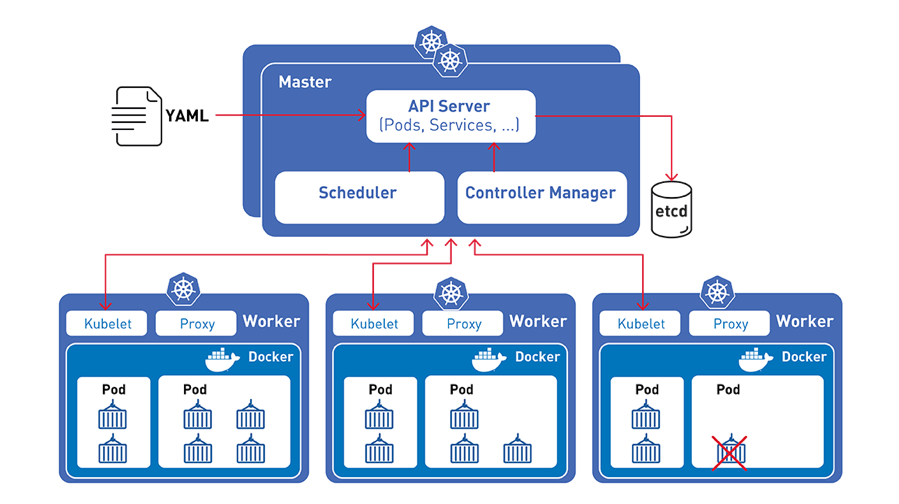
\includegraphics[width=0.8\linewidth]{figures/k8s_architecture.png}
    \caption[Kubernetes Architecture]{This diagram from~\textcite{k8sDiagram} shows the structure of a Kubernetes cluster.}
    \label{fig:k8sArchitecture}
\end{center}
\end{figure}


Kubernetes is a highly flexible and configurable system for container orchestration that provides automatic deployment, scaling, and administration of container applications, as explained in the \textcite{k8sdocs}. 

\paragraph{Architecture}

The Kubernetes architecture is depicted in Figure \ref{fig:k8sArchitecture}. It shows a \textit{cluster}, which is a set of \textit{nodes}\footnote{\url{https://kubernetes.io/docs/concepts/architecture/nodes/}, accessed 2019-07-19} that run the container applications. Nodes can either be physical or virtual machines, the latter being especially prevalent in hosted public cloud scenarios. Every cluster consists of at least one master and one worker node. 

The master nodes run all so-called \textit{control plane components} that are necessary for the cluster to function. These include the \textit{API server} and \mycode{etcd}. The \textit{API server} exposes the \textit{Kubernetes API}\footnote{\url{https://kubernetes.io/docs/concepts/overview/kubernetes-api/}, accessed 2019-07-19}, which is used to control the cluster state. Administrators typically interact with the API using the CLI tool \mycode{kubectl}\footnote{\url{https://kubernetes.io/docs/reference/kubectl/overview/}, accessed 2019-07-19}. The central key-value database \mycode{etcd}\footnote{\url{https://etcd.io}, accessed 2019-07-25} stores all cluster information and is only supposed to be accessed directly by the API server.

Worker nodes run the container daemon and the \textit{kubelet}, which is an agent responsible for managing the node. On the workers, the actual containerised applications run. The containers reside within \textit{pods}\footnote{\url{https://kubernetes.io/docs/concepts/workloads/pods/pod/}, accessed 2019-07-19}. A pod runs one or more containers on the same node. Pods are the smallest units that can be scheduled to run. They, like all other Kubernetes objects, are declaratively specified in the \textit{YAML} format\footnote{\url{https://yaml.org}, accessed 2019-07-19}. These specifications include the URL to the container images in the registry, metadata and configuration information. Examples of specification files are given throughout this thesis and in Appendix A. To create a pod, its specification is submitted to the Kubernetes API. The control plane takes care of the deployment and scheduling of the specified pod. 

\paragraph{Scaling}

The power of Kubernetes lies in its more advanced concepts, including \textit{Deployments}\footnote{\url{https://kubernetes.io/docs/concepts/workloads/controllers/deployment/}, \\ accessed 2019-07-19} and \textit{ReplicaSets}\footnote{\url{https://kubernetes.io/docs/concepts/workloads/controllers/replicaset/}, \\ accessed 2019-07-19}. These can be used to define how multiple instances of pods should be run. Kubernetes then takes care that the cluster is always in the desired state, updates are rolled out, and new replicas are spun up if required.

\paragraph{Configuration and Secrets Management}

For configuration and credentials management, Kubernetes provides the objects \textit{ConfigMap} and \textit{Secret}\footnote{\url{https://kubectl.docs.kubernetes.io/pages/app_management/secrets_and_configmaps.html}, accessed 2019-07-18}, which can be configured using YAML specifications. They are then mounted into the containers' file systems or passed along using environment variables so that applications can retrieve them.

\paragraph{Exposing applications}

To expose applications running on a set of pods, \textit{services}\footnote{\url{https://kubernetes.io/docs/concepts/services-networking/service/}, accessed 2019-07-18} can be used. They can either be employed for internal communication within the cluster or can be bound to an \textit{ingress}\footnote{\url{https://kubernetes.io/docs/concepts/services-networking/ingress/}, accessed 2019-07-19} to expose them to the public internet. 

%% vim:foldmethod=expr
%% vim:fde=getline(v\:lnum)=~'^%%%%\ .\\+'?'>1'\:'='
%%% Local Variables: 
%%% mode: latex
%%% mode: auto-fill
%%% mode: flyspell
%%% eval: (ispell-change-dictionary "en_US")
%%% TeX-master: "main"
%%% End: 

%% example text content
%% scrartcl and scrreprt starts with section, subsection, subsubsection, ...
%% scrbook starts with part (optional), chapter, section, ...
\chapter{Kubernetes Cluster Security}\label{chap:clusterSecurity}

In Kubernetes there are many aspects to consider when looking at it from a security perspective. With its flexibility also comes considerable complexity. In order to come by it and discuss it in a structured manner, we have created the model depicted in Figure~\ref{fig:secmodel}. It is aimed at giving a holistic view over all aspects that might influence the security of a Kubernetes cluster and uses structure ideas from~\textcite{securingkubernetes} and~\textcite{kubernetessecurity}.

\myfig{layers.pdf} %% filename in figures folder
  {width=1.0\textwidth,height=0.6\textheight}%% maximum width/height, aspect ratio will be kept
  {This security model shows the different layers that have to be considered when holistically regarding Kubernetes security.}%% caption
  {Security Model}%% optional (short) caption for table of figures
  {fig:secmodel}%% label

The model is composed of the following four layers:

\begin{enumerate}
    \item The lowest layer we call \textbf{Base Infrastructure Security} and it concerns all components on which Kubernetes itself builds. These include the Operating System, the container engine (most likely Docker), and the infrastructure of the public or private cloud provider when for example using Google Cloud Platform or Amazon Web Services as an \textit{\ac{IaaS}} provider. This layer is described in Section~\ref{sec:layer1}.
    \item Upon that builds \textbf{Kubernetes Infrastructure Security} which is described in detail in Section~\ref{sec:layer2}. It concerns everything related to Kubernetes' control plane components and their configuration in terms of security. Potential issues there include abuse of the internal Kubernetes APIs, such as the Kubelet API, or intercepting internal traffic between control plane components.
    \item Additionally to the configuration of the Kubernetes control plane components themselves, there are also security components provided by Kubernetes to secure clusters. These components include Kubernetes' authentication and authorisation mechanisms, pod security policies, secrets management and many more. We group them together in the layer \textbf{Kubernetes Security Controls} as described in Section~\ref{sec:layer3}.
    \item The top-most layer is called \textbf{App and Container Security} and makes use of all layers underneath it. On this layer, the actual applications run in containers, which in turn are located in pods. Exploiting of vulnerabilities in the application code might breach this layer. These topics are described in detail in Section~\ref{sec:layer4}.
\end{enumerate}

The layered architecture also makes sense when considering damage control aspects of Kubernetes security: As one layer on the top breaches, the lower layers can still prevent further damage. For example, when there is a vulnerability in the application code on layer 4, a properly configured set of permissions on layer 3 for the pod might still prevent further damage. Inversely, an insecure port left open in a control plane component, such as the API server, on layer 2 might allow an attacker to infiltrate a whole cluster, taking over all pods, containers and applications on the upper layers. 
	
\section{Base Infrastructure Security} \label{sec:layer1}

The base infrastructure, in which a Kubernetes cluster is run, sets the foundation for the whole cluster's security, as explained in~\textcite{securingkubernetesBaseInfra}. However well-tuned the Kubernetes cluster configuration is, a breach in the underlying infrastructure of a Kubernetes node can compromise the whole cluster. Depending on whether a cluster runs in a public or private cloud environment, some of the following guidelines may apply. When a cluster runs in a managed environment, such as on Google Kubernetes Engine (GKE) or Amazon Elastic Container Service for Kubernetes (Amazon EKS), a lot of this configuration may already be taken care of by the provider.

\paragraph{Operating System}

Every component in Kubernetes is run by an underlying operating system, mostly a flavour of Linux. While vulnerabilities in the OS itself are outside the scope of this thesis, some general guidelines should be followed to minimise the risk of a breach on OS level:

\begin{itemize}
    \item An operating system with container support that has a minimal attack surface should be used, such as \textit{CoreOS Container Linux}\footnote{\url{https://coreos.com/os/docs/latest/}, accessed 2019-06-10} or \textit{k3OS}\footnote{\url{https://k3os.io}, accessed 2019-06-10} that has been specifically designed for Kubernetes.
    \item Just like Kubernetes should be regularly patched, the operating system kernel should also be running at the most recent version at all times.
    \item For many Linux distributions there are hardening guides that can be used as a reference for the system configuration, such as the \textit{CoreOS Container Linux hardening guide}\footnote{\url{https://coreos.com/os/docs/latest/hardening-guide.html}, accessed 2019-06-10}. 
\end{itemize}

\paragraph{Container Runtime}

Upon the OS builds the container runtime in which all containers are run in the cluster. At the time of this writing, mostly the runtime is \textit{Docker}\footnote{\url{https://www.docker.com}, accessed 2019-06-10}, but also alternatives that comply with the \textit{Kubernetes Container Runtime Interface}\footnote{\url{https://kubernetes.io/blog/2016/12/container-runtime-interface-cri-in-kubernetes/}, accessed 2019-06-10} such as \textit{containerd}\footnote{\url{https://containerd.io}, accessed 2019-06-10} gain traction.

Besides the OS, also the container runtime should always be up-to-date and configured securely. It is essential not to forget about it in the stack and acknowledge that containers are not virtual machines and do not provide the same kind of isolation. A breach out of a container can, therefore, mean that not only a pod, but an entire node can be compromised.

\paragraph{Network environment}

Outside access to cluster resources should be as restricted as possible. In most configurations, access to functionality provided by the cluster is exposed only via Kubernetes Services. Hence it is neither necessary nor recommended for every node to be exposed to the public internet. The attack surface of the whole cluster can, therefore, be reduced by putting all nodes in a private network and exposing only the services via a load balancer.

\paragraph{Trusted Platform Modules}

\acp{TPM}, as standardised in~\textcite{TPMStandard}, can be a powerful addition to the base infrastructure to increase its security. As demonstrated by~\textcite{TPM}, \acp{TPM} can be used to store cryptographic keys that stay secure from an attacker even if an entire node is compromised. 

\section{Kubernetes Infrastructure Security} \label{sec:layer2}

The security of Kubernetes infrastructure concerns the configuration of all components of the Kubernetes control plane and their internal communications. When setting up and administering a cluster, there are many configurations that, at first sight, do not appear to be critical to security. Still, the following aspects must not be neglected to ensure a secure cluster setup. Many best practice guidelines are listed in~\textcite{kubernetessecurity}.

\subsection{Cluster installers}

While it is possible to set up a cluster completely manually\footnote{\url{https://github.com/kelseyhightower/kubernetes-the-hard-way}, accessed 2019-06-11}, most are set up using cluster installers such as \mycode{kubeadm}\footnote{\url{https://kubernetes.io/docs/setup/independent/create-cluster-kubeadm/}, accessed 2019-06-11} or \mycode{kops}\footnote{\url{https://github.com/kubernetes/kops}, accessed 2019-06-11}. They can be used to bootstrap all control plane components, set up the \ac{PKI} and network configuration, and join worker nodes to the cluster.

Even though most installers come with sane default configurations, it is crucial to verify them and check what is done under the hood, as emphasised by~\textcite{securingkubernetesConfK8SClusterComponents}. 

\subsection{API server}

The API server is an essential control plane component, as an attacker that gains control over it has the equivalent of root access to the whole cluster, as described by~\cite{kubernetessecurity}. The critical aspect of how the API itself is secured and how the API server fulfils its role as the cluster's \ac{CA} is described in Section \ref{sec:apiAccessControl}, as this resembles a Kubernetes security control and is therefore grouped in the corresponding layer of our model. 

Still, any misconfiguration of the API server might mean leaving the front door to the cluster open, which is why its configuration should always be reviewed from a security perspective. This includes the fact that the Kubernetes API should generally not be exposed to the public internet if there is no pressing need.

\subsection{Kubelets}

A Kubelet is an agent running on every node that is responsible for running its containers, reporting metrics and similar. It receives its commands from the control plane. For that, it provides the so-called \textit{Kubelet API}, which is undocumented, as it is not supposed to be used by anyone other than the control plane. 

This API needs to be adequately protected, as otherwise it can be misused as shown by~\textcite{kubeletBackdoor}. This misconfiguration gave any attacker with network access to nodes an unauthenticated API backdoor to the cluster. In the Kubernetes version 1.15, which is the most current one at the time of this writing, the API is protected by default. The insecure port is closed and the secure ones calls back to the API server to verify whether a request should be allowed (see \textit{Node Authorisation} in Section \ref{ssec:authorisation}). 

It is worth noting that disallowing node network access, as recommended in Section \ref{sec:layer1}, could have prevented this exploit in the first place.

\subsection{etcd}\label{ssec:etcd}

\mycode{etcd} is the central storage location in Kubernetes that stores all cluster data in a key-value data structure. The API server is the only component that is supposed to access it directly.

\paragraph{Access restriction}
In order to enforce that only the API server can communicate with \mycode{etcd}, network policies, as later described in Section~\ref{ssec:networking}, should set up and an adequate certificate configuration\footnote{\url{https://github.com/etcd-io/etcd/blob/master/Documentation/op-guide/security.md}, accessed 2019-06-11} should be put in place.

\paragraph{Encryption}
By default, all data in \mycode{etcd} is stored in plain text. As it also stores all secrets, sensitive information might be exposed, if the data on the volume used by \mycode{etcd} leaks. In order to mitigate that, encryption can and should be enabled by providing the API server with an encryption configuration using the startup parameter \mycode{--encryption-provider-config} as described in the \textcite{k8sdocs}\footnote{\url{https://kubernetes.io/docs/tasks/administer-cluster/encrypt-data/}, accessed 2019-06-11}.


\subsection{Kubernetes Dashboard}

The Dashboard\footnote{\url{https://kubernetes.io/docs/tasks/access-application-cluster/web-ui-dashboard/}, accessed 2019-07-19} is a Web UI for administrating a Kubernetes cluster and gives a convenient overview over the pods, deployments, services and other objects currently deployed. However, in a recent incident at Tesla, described in~\textcite{teslaLeak}, a cluster was compromised due to an insufficiently secured Dashboard and used for crypto mining. This illustrates how leaving it exposed to the public internet or leaving it configured insecurely can compromise the security of an entire cluster. Therefore~\textcite{kubernetessecurity} suggest to follow these guidelines to secure it:

\begin{itemize}
    \item Only authenticated users should be allowed access.
    \item The service account the Dashboard is using should have limited privileges so that users cannot misuse its permissions and rather log in with their own users.
    \item The dashboard should not be exposed to the public internet.
\end{itemize}

\section{Kubernetes Security Controls} \label{sec:layer3}

Kubernetes provides cluster operators with an extensive set of options and tools to tweak the security of a cluster. These build upon the Kubernetes and base infrastructure and are very important to configure correctly. 

\subsection{Namespaces} \label{sec:namespaces}

As described in the~\textcite{k8sdocs}\footnote{\url{https://kubernetes.io/docs/concepts/overview/working-with-objects/namespaces/}, accessed 2019-05-31}, almost every resource in a Kubernetes cluster belongs to a namespace. Exceptions include only namespaces themselves and some low-level resources such as nodes. 

All resources belonging to the control plane components reside within the \mycode{kube-system} namespace, while by default all other objects are located in the \mycode{default} namespace. 

Generally, namespaces can be used to avoid naming conflicts, but also to allow for finer grained access control. For example, using API access control, a role can be created so that a user can list all pods from a particular namespace, but not for any other namespace, as further described in Section~\ref{sec:apiAccessControl}. Using this feature makes sense primarily when the cluster is used by a large number of users from, for example, different projects or departments. 

Namespaces can sometimes alleviate the need for creating separate clusters to isolate components from each other. Some use cases might include different namespaces per team, application or environment (such as different namespaces for development, testing and production). 

However, as pointed out in~\textcite{namespacesInsights}, while namespaces are suited well for logical partitioning and assigning permission sets on API access level, they do not enforce the partitioning by setting firewall rules or such. Any cluster user or resource can access any other resource in the cluster, even when they are in different namespaces. To achieve partitioning on the network level, see Section~\ref{ssec:networking}.

\subsection{API Access Control} \label{sec:apiAccessControl}

As explained in Chapter \ref{cha:background}, the only component in a Kubernetes cluster that is allowed to modify the cluster state in \mycode{etcd} directly is the API server. Therefore all requests that involve reading or modifying the cluster state must be performed via the Kubernetes API. It is well-documented in~\textcite{k8sdocsApi} and is very powerful, as it is also used by all control plane components to communicate with each other. Hence it needs to be carefully protected from unauthorised access. The API server achieves that using three steps to very if and how a request should be performed, as depicted in Figure~\ref{fig:apiServerAccessControl}.

\myfig{api_access_control_itnext.png}{width=0.8\textwidth}{This image from~\textcite{securingkubernetesConfK8SClusterComponents} displays the steps performed by the API server before it persists a request made to it.}{API server access control flow}{fig:apiServerAccessControl}

First, \textbf{Authentication} is performed to determine the identity of the user or system that is trying to access the API. After the identity of the accessing party has been determined, \textbf{Authorisation} is used to decide whether they are allowed to access or modify the requested resource. Finally \textbf{Admission Controllers} are applied to the request to validate or mutate it, before it is ultimately persisted.

\subsubsection{Authentication} \label{ssec:authentication}

Users in Kubernetes can be either Service Accounts or normal (human) users. 

Service Accounts are managed directly by Kubernetes and give identities to apps running inside pods as described in~\textcite{k8sdocs}\footnote{\url{https://kubernetes.io/docs/tasks/configure-pod-container/configure-service-account/}, accessed 2019-06-10}. With these identities, the applications can access the API server. Service Accounts are Kubernetes objects and are stored in \mycode{etcd}. A pod can be configured to use a particular service account, which results in the corresponding certificates being mounted into the pod's file system. With these, the application running in it can authenticate with the API server. 

For human users, no Kubernetes objects in \mycode{etcd} exist. The administration of those is outsourced to an external entity. The API server offers multiple strategies to authenticate such users, a subset of which are the following:

\begin{itemize}
    \item The default way of authentication between control plane components is using \textbf{X.509 certificates} within the \ac{PKI} of the cluster. For that to function, the API server is handed the \ac{CA} file using the start-up parameter \mycode{--client-ca-file= /path/to/ca.crt}. Users can then authenticate using a certificate signed by the provided \ac{CA}.
    
    At the time of this writing, however, Kubernetes does not have support for \ac{CRL} or \ac{OCSP}, with which certificates could be revoked. The issue is currently under debate within the Kubernetes developer community\footnote{\url{https://github.com/kubernetes/kubernetes/issues/18982}, accessed 2019-05-28}. In the meantime, authorisation has to be used to strip users from permissions retroactively.

    \item An \textbf{Authentication Proxy} can be used to outsource the task of authentication to an external entity that might run within our outside of the cluster.
    
    \item In order to enable support for \ac{SSO}, the API server can be configured to use \textbf{\ac{OIDC}}\footnote{\url{https://openid.net/connect/}, accessed 2019-05-28} for authentication. It builds upon the OAuth 2.0 flow and allows the use of external identity providers that implement the standard, such as the common \textit{"Sign in with Facebook/Google/Microsoft"} known from various places on the web. 

   \item For testing and demo purposes it is also possible to use a \textbf{static password file} as per the definition in the RFC 7617 "The 'Basic' HTTP Authentication Scheme" by~\textcite{RFC7617}. However, it is rarely practical in real-world use cases as the password file needs to be maintained manually.
	
\end{itemize}

Authentication considers no actual permissions. It only determines the identity of the authenticating entity and several attributes about it, such as the username and group memberships. This information is passed on to the next step, authorisation, in which the actual mapping step of who is allowed to do what happens. 

\subsubsection{Authorisation} \label{ssec:authorisation}

As is the case for authentication, Kubernetes also provides several options for how authorisation can be performed as defined in the documentation~\textcite{k8sdocs}\footnote{\url{https://kubernetes.io/docs/reference/access-authn-authz/authorization/}, accessed 2019-05-31}:

\begin{itemize}
    \item \textbf{Node Authorisation} is used only by \mycode{kubelet}s, so that nodes are equipped with the minimum set of permissions they need to operate within the cluster.
    \item \textbf{\ac{ABAC}} grants permissions by explicit policies based on the users' attributes, such as name, location or department. \ac{ABAC}, however, has been deprecated since Kubernetes version 1.6 and is not recommended to be used anymore.
    \item \textbf{\ac{RBAC}} defines roles that come with certain permissions. These roles can then be bound to users to grant them access.
    \item \textbf{Webhook Mode} queries an external REST service to outsource the authorisation to it.
\end{itemize}

As~\textcite{ABACvsRBAC} point out, conceptually there are advantages and disadvantages to both \ac{ABAC} and \ac{RBAC}. While \ac{ABAC} provides more flexibility, \ac{RBAC} lends itself better for analysis and risk assessment. The main advantage of \ac{ABAC} is that it can perform restrictions directly based on users' attributes. In the context of Kubernetes, however, its developers~\textcite{ABACvsRBACk8s} argue that only \ac{RBAC} should be used anymore. That is acceptable primarily as the third step of API access control in Kubernetes, \textit{Admission Control}, can provide filters to accommodate for such finer-grained control.

\ac{RBAC} is the recommended way of performing authorisation at the time of this writing, as it is easier to understand and configure than \ac{ABAC} while retaining most of its configuration power. Therefore, we will only consider it in this work and disregard the other options.

\paragraph{\ac{RBAC}}

\myfig{rbac.png}{width=0.5\textwidth}{This graphic from~\textcite{k8sCookBook} depicts the basic building blocks of \ac{RBAC}.}{RBAC building blocks}{fig:rbac}

The basic building blocks of \ac{RBAC} are depicted in Figure \ref{fig:rbac}. \textit{Roles} are used to define access to certain \textit{Resources}. Rules can either be defined cluster-wide or namespace wide, depending on the objects they control access to.

A role that allows reading pods is created by applying a YAML file like this: 

\begin{minted}[
    autogobble,
    frame=single,
    linenos
  ]{yaml}
kind: Role
apiVersion: rbac.authorization.k8s.io/v1
metadata:
  name: pod-reader
  namespace: default
rules:
- apiGroups: [""]
  resources: ["pods"]
  verbs: ["get", "watch", "list"]
\end{minted}

Besides some metadata, a role defines certain API groups (in the above example the \mycode{""} indicate the core API), resources and certain verbs that correspond to the actions that are allowed on the resource. 

In order to assign the role to an \textit{Entity}, in this example case a \mycode{ServiceAccount} called \mycode{example-app-sa}, a \textit{RoleBinding} for the namespace \mycode{default} can be created by applying a YAML file like this:

\begin{minted}[
    autogobble,
    frame=single,
    linenos
  ]{yaml}
kind: RoleBinding
apiVersion: rbac.authorization.k8s.io/v1
metadata:
  name: read-pods
  namespace: default
subjects:
- kind: ServiceAccount
  name: example-app-sa 
  namespace: default
roleRef:
  kind: Role
  name: pod-reader
  apiGroup: rbac.authorization.k8s.io
\end{minted}

Besides \textit{Roles} and \textit{RoleBindings}, there are also \textit{ClusterRoles} and \textit{ClusterRoleBindings} that work similarly, just that they manage permissions on the scope of the whole cluster instead of being bound to a specific namespace.

As for all security configurations, the principle of Least Privilege applies especially when it comes to the configuration of \ac{RBAC}. It has been initially defined by~\textcite{leastPrivilege} as \enquote{Every program and every privileged user of the system should operate using the least amount of privilege necessary to complete the job.}. 

Applied to Kubernetes API access control, this means that an application which does not need to access the Kubernetes API to function, as is likely the case for the vast majority of applications, should not be allowed to do so. As pointed out by \textcite{kubernetessecurity}, it is therefore recommended to disable the auto-mounting of the default Service Account into pods by setting \mycode{automountServiceAccountToken: false} in the pod specification. 

Section \ref{ssec:exaLayer3}. shows another practical example of an \ac{RBAC} configuration that adheres to this principle.

\subsubsection{Admission Control} \label{ssec:admissionControl}

As described in \cite{admissionControl} and \cite{k8sdocs}\footnote{\url{https://kubernetes.io/docs/reference/access-authn-authz/admission-controllers/}, accessed 2019-05-25}, admission control allows for a set of plug-ins to enforce rules about how a cluster is used, by being applied after a request to the API server has passed authentication and authorisation. These plug-ins can be either \textit{mutating}, \textit{validating} or both. First, all mutating admission controllers are executed, then the validating controllers. If any of them rejects the request, the processing is aborted and the request is rejected.

An especially important admission controller with respect to security is the built-in \mycode{PodSecurityPolicy}. It can be used to forbid containers running with privileged users or set containers' file systems to read-only. Both of these are sensible best practices, as further explained in the context of container security in Section \ref{ssec:exaLayer4}.

Besides standard admission controllers that ship with Kubernetes and should be disabled or altered only under certain circumstances, there is also support for custom controllers that build upon the standard \mycode{MutatingAdmissionWebhook} or \mycode{ValidatingAdmissionWebhook}. These allow for high flexibility as their admission is based on a REST call to a service running within the cluster. This feature can be used to develop custom restrictions, such as this example\footnote{\url{https://github.com/stackrox/admission-controller-webhook-demo}, accessed 2019-05-28} that causes all containers to be run with a non-root user, except they are explicitly marked to do otherwise. 

\subsection{Networking} \label{ssec:networking}

Communication between Kubernetes components and the outside world is a central aspect for Kubernetes to function. As described in detail in the article series \textcite{NetworkingExplained} and in the documentation \textcite{k8sdocs}\footnote{\url{https://kubernetes.io/docs/concepts/cluster-administration/networking/}, accessed 2019-06-10}, it can be broken down in to several aspects:

\begin{itemize}
    \item Containers within the same pod communicate with each other via localhost.
    \item Pods communicate with other pods and with the control plane adhering to the Kubernetes Networking model\footnote{\url{https://kubernetes.io/docs/concepts/cluster-administration/networking/\#the-kubernetes-network-model}, accessed 2019-06-10} that defines an overlay network for that purpose. The model is aimed to be very flexible and should allow for easy porting from virtual machines. It mainly builds upon the premise that pods can be addressed with their own IP addresses, despite multiple pods running on the same node. The network model is not directly implemented in the Kubernetes core, but rather different plug-ins can be used to meet its requirements. These plug-ins integrate with nodes and their kernels to establish the layer 3 (network layer) communication as defined in~\textcite{osiModel}.
    \item Communication with the outside world is handled by services that can be bound to  Ingress\footnote{\url{https://kubernetes.io/docs/concepts/services-networking/ingress/}, accessed 2019-06-10} objects.
\end{itemize}

From a security perspective, an especially important topic in networking are Network Policies\footnote{\url{https://kubernetes.io/docs/concepts/services-networking/network-policies/}, accessed 2019-05-28}, which allow configuration on which pods are allowed to communicate with each other and with other network endpoints. Network policies are realised in the Kubernetes object \mycode{NetworkPolicy}. Still, not all networking plug-ins support them.

An example for a \mycode{NetworkPolicy} could look like this:

\begin{minted}[
    autogobble,
    frame=single,
    linenos
  ]{yaml}
  kind: NetworkPolicy
  apiVersion: networking.k8s.io/v1
  metadata:
    name: example-policy
  spec:
    podSelector:
      matchLabels:
        app: example-app
    policyTypes:
    - Egress
    - Ingress
    ingress:
    - from:
      - podSelector:
          matchLabels:
            access: "true"
\end{minted}

The \mycode{policyTypes} specify whether egress traffic, ingress traffic or both are affected by this policy. The white-list principle applies so that only the specified traffic is allowed. This example applies to all pods with the label \mycode{app} set to \mycode{example-app}. It allows incoming traffic only from pods with the label \mycode{access} set to \mycode{true} and prohibits all outgoing traffic.

In most cases, it makes sense to prohibit egress by default. In this case, even if a pod is entirely hijacked, it cannot directly communicate with the outside world via a reverse shell (connect-back shell). Of course, however, such a restriction could be bypassed by using a bind shell that listens on a specific port for an incoming connection from the attacker as explained in~\textcite{bindAndReverseShells}. Still, such an approach would require more effort from the attacker.

An example of how Network Policies can be used to secure a real-world cluster is given in Section \ref{ssec:exaLayer3}.

\section{App and Container Security} \label{sec:layer4}

The top-most layer of the model concerns the applications that run in the Kubernetes cluster within their container environments. Their security relies on the lower layers while also being protected by them.

\subsection{Application Security}

The largest attack surface on this layer naturally are the applications themselves. As the whole class of application vulnerabilities cannot be mitigated entirely, Kubernetes provides many damage control tools on lower levels that limit an attacker's possibilities, even when an application has been compromised. This is a good practice example of defence in depth, as explained in~\textcite{defenceInDepth}.

\paragraph{Image Scanning} 

Often, the containers that are run in a cluster build upon public images and included application packages. Image scanning tools, such as \textit{Anchore Engine}\footnote{\url{https://github.com/anchore/anchore-engine}, accessed 2019-06-28} and \textit{Clair}\footnote{\url{https://github.com/coreos/clair}, accessed 2019-06-28}, scan images before they are deployed and analyse whether they contain known vulnerabilities. Using the admission controller \mycode{ImagePolicyWebhook}, as explained in Section~\ref{ssec:admissionControl}, API access control can be configured to refuse the deployment of images for which vulnerabilities are reported.  

\subsection{Container Configuration}

In this section, several precautions are explained that can be taken on container level to increase cluster security.

\paragraph{Non-privileged containers}

As pointed out in detail in~\textcite{nonPrivContainers}, applications in containers should run with non-privileged users, as most of them should not require root permissions. This restriction can be enforced by adding the following statements to the \mycode{PodSecurityPolicy} configuration:

\begin{minted}[
    autogobble,
    frame=single,
    linenos
  ]{yaml}
allowPrivilegeEscalation: false
runAsUser:
  rule: 'MustRunAsNonRoot'
\end{minted}

One side effect of not running as root is that applications can not bind to well-known ports ($< 1024$), but this can be easily mitigated by using the port binding capabilities of the container runtime.

\paragraph{Minimal containers}

Containers should only run the bare minimum of applications they require to fulfil their aim. It is therefore considered bad practice to run, for example, an SSH server to do maintenance work, as explained in~\textcite{noSSHDinContainers}. Most actions that would require having an SSH server running can also be achieved using Kubernetes features.

\paragraph{Secrets and Configuration}

Secrets and configuration items should not be baked into the container images, but should instead be managed using the Kubernetes objects \mycode{Secret} and \mycode{ConfigMap} respectively. These can then either be exposed to the containers using environment variables or by mounting them to a volume accessible to the container. By doing so, they can be more easily adapted and are not prone to leak when a container image leaks.

\paragraph{Rule-based Execution}

As explained in the~\textcite{k8sdocs}\footnote{\url{https://kubernetes.io/docs/concepts/policy/pod-security-policy/}, accessed 2019-06-25}, a \mycode{PodSecurityPolicy} can be used to enforce several rule-based execution restrictions. The configuration options include:

\begin{itemize}
    \item \mycode{seccomp}, as documented in~\textcite{seccompMan}, can limit the allowed system calls for user-space applications. At the time of this writing, \mycode{seccomp} is disabled by default in Kubernetes so that even the default Docker profile\footnote{\url{https://docs.docker.com/engine/security/seccomp/}, accessed 2019-06-28} does not apply.
    \item Policies of SELinux\footnote{\url{https://selinuxproject.org/page/Main_Page}, accessed 2019-06-25} and AppArmor\footnote{\url{https://kubernetes.io/docs/tutorials/clusters/apparmor/}, accessed 2019-06-25} can be configured for finer-grained access control. 
    \item Linux capabilities, as explained in~\textcite{linuxCaps}, are a kernel feature that can grant a process running as root some, but not all privileged capabilities. In Kubernetes, the whitelist of capabilities that can be added to a container can be configured.
\end{itemize}

%% vim:foldmethod=expr
%% vim:fde=getline(v\:lnum)=~'^%%%%\ .\\+'?'>1'\:'='
%%% Local Variables: 
%%% mode: latex
%%% mode: auto-fill
%%% mode: flyspell
%%% eval: (ispell-change-dictionary "en_US")
%%% TeX-master: "main"
%%% End: 

%% example text content
%% scrartcl and scrreprt starts with section, subsection, subsubsection, ...
%% scrbook starts with part (optional), chapter, section, ...
\chapter{Securing an Example Application} \label{chap:example}

In this chapter, the security concepts introduced above are put into practice by applying them to a real-world application. This application has been created solely for demonstration purposes to resemble a use case that makes extensive use of Kubernetes' features while still retaining simplicity to be generally applicable and easy to understand. The full configuration files of the application can be found in Appendix A.

\section{Example Application}

\paragraph{Functionality}

The example application is a simple dashboard for Kubernetes to view Pods in certain or all namespaces. It can also display and scale ReplicaSets. A screenshot of it is depicted in Figure \ref{fig:exaScreenshot}. For providing this functionality, it queries the API server for information, communicates between different components using services and exposes its functionality via an ingress. 

\begin{figure}[H]
\begin{center}
    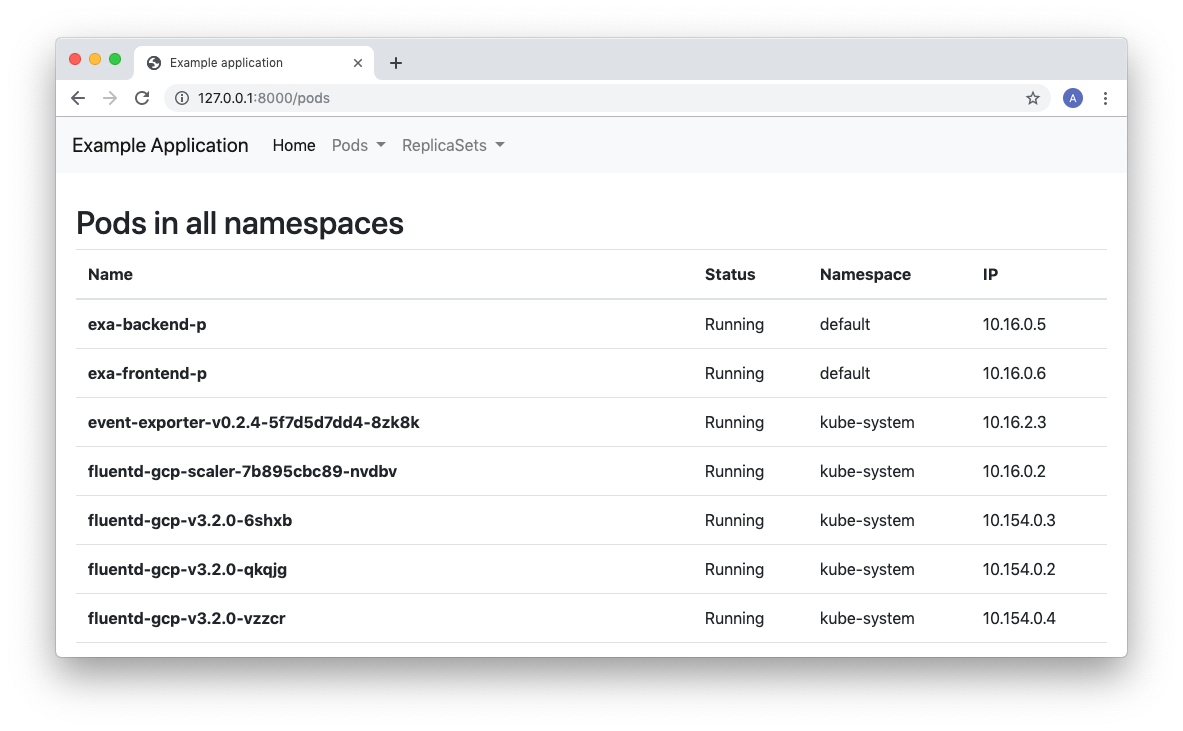
\includegraphics[width=1.0\linewidth]{figures/exa_screenshot.png}
    \caption[Screenshot of the example application]{This screenshot depicts the front page of the example application.}
    \label{fig:exaScreenshot}
\end{center}
\end{figure}

\paragraph{Setup}

The application is written in Python and makes use of Flask\footnote{\url{http://flask.pocoo.org/}, accessed 2019-07-02} as well as the Kubernetes Python Client\footnote{\url{https://github.com/kubernetes-client/python}, accessed 2019-07-02}. 

The setup consists of a backend part, \mycode{exa-backend}, and a frontend part, \mycode{exa-frontend}. \mycode{exa-backend} provides a REST API and directly accesses the Kubernetes API, while \mycode{exa-frontend} uses the backend for retrieving the data. 

\begin{figure}[H]
\begin{center}
    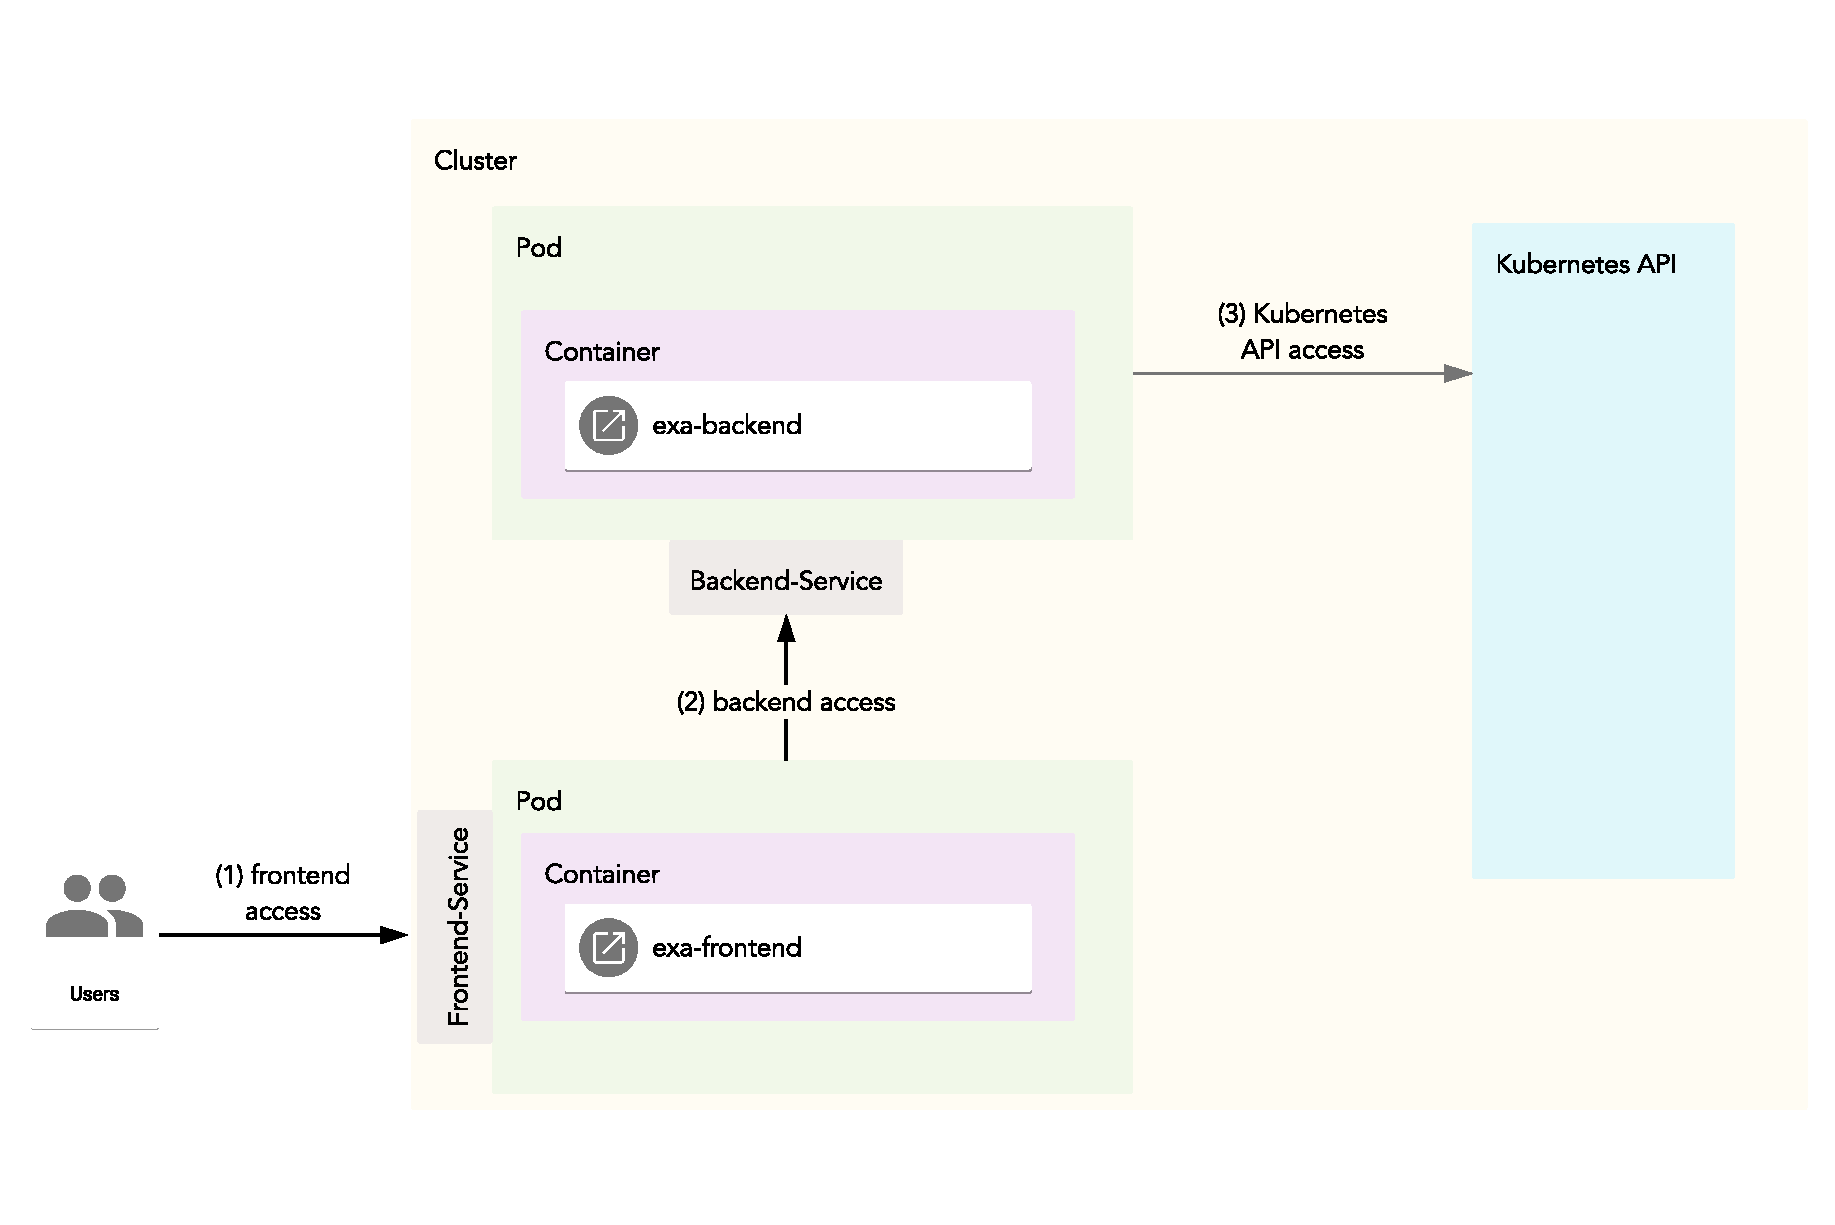
\includegraphics[width=1.0\linewidth]{figures/exa_architecture.pdf}
    \caption[Architecture of the example application]{This architecture diagram shows how the example application runs within the Kubernetes cluster.}
    \label{fig:exaArchitecture}
\end{center}
\end{figure}

% TODO reduce mentions of GKE, don't want it to sound like marketing

The Kubernetes cluster is run in \ac{GKE} on \ac{GCP}\footnote{\url{https://cloud.google.com/kubernetes-engine/}, accessed 2019-07-02}. It is a sensible choice for cluster administrators who are not yet experts in the field of Kubernetes security, as it scales well from a very basic setup up to a large high-availability cluster. 

The architecture of the cluster is depicted in Figure~\ref{fig:exaArchitecture}. The frontend and backend components run in separate pods. Users access the frontend via an ingress that maps to the frontend service. The frontend then retrieves all information by calling the backend service, which in turn makes the request to the Kubernetes API to perform the user's query. We are choosing this setup intentionally so that the frontend does not have direct access to the API to resemble a typical frontend-backend architecture. The following sections describe how we use Kubernetes to enforce these environment restrictions.

\section{Security Measures}

In this section, the measures that were taken to secure the setup are explained. They are structured according to the layer model introduced in Chapter~\ref{chap:clusterSecurity}.

\subsection{Base Infrastructure Security}

As this setup uses \ac{GKE} as an infrastructure provider, most considerations for base infrastructure security are already taken care of by Google\footnote{\url{https://cloud.google.com/kubernetes-engine/docs/concepts/security-overview}, accessed 2019-07-09}. By default, \ac{GKE} clusters run the newest version of Google's Container-Optimized OS\footnote{\url{https://cloud.google.com/container-optimized-os/docs/concepts/features-and-benefits}, accessed 2019-07-09} that comes with a current version of the container runtime as well. 

However, as all cluster components are running within the \ac{GCP} environment, they are also subject to Google's Cloud \ac{IAM}\footnote{\url{https://cloud.google.com/iam/}, accessed 2019-07-09}. It works alongside Kubernetes \ac{RBAC}, yet requires some special attention when applications within the Kubernetes cluster access other resources on \ac{GCP} outside of the cluster.\footnote{\url{https://cloud.google.com/kubernetes-engine/docs/how-to/iam}, accessed 2019-07-09}

\subsection{Kubernetes Infrastructure Security}

When it comes to Kubernetes' infrastructure components, most relevant security aspects are still closely tied to the underlying base infrastructure, in this case, \ac{GKE}.

\paragraph{API Server}

The aforementioned \ac{IAM}, by default, allows login using username and password. We disable it in the cluster configuration in the \ac{GCP} web interface and only used certificates, which we regularly rotate\footnote{\url{https://cloud.google.com/kubernetes-engine/docs/how-to/credential-rotation}, accessed 2019-07-09}, to authenticate within the cluster.

\paragraph{Secret Encryption}

As explained in Section~\ref{ssec:etcd}, it is vital to encrypt all secrets stored in \mycode{etcd}. \ac{GKE} already provides encryption at rest by default\footnote{\url{https://cloud.google.com/security/encryption-at-rest/default-encryption/}, accessed 2019-07-09}, in case an attacker gains access to an offline copy of the \mycode{etcd} database. However, to protect against the case that an attacker gains online access to the machine that runs \mycode{etcd}, we also configure application-layer encryption. To set it up, we generate a key, store it in Google's Cloud Key Management Service (KMS)\footnote{\url{https://cloud.google.com/kms/docs/}, accessed 2019-07-09} and hand it to the cluster configuration using \mycode{--database-encryption-key}\footnote{\url{https://cloud.google.com/kubernetes-engine/docs/how-to/encrypting-secrets}, accessed 2019-07-09}.  

\paragraph{Dashboard}

As the standard Kubernetes dashboard is deprecated and disabled by default on \ac{GKE}, no further configuration was necessary to secure the setup. The \ac{GCP} Console\footnote{\url{https://console.cloud.google.com/}, accessed 2019-07-09}, which acts as a replacement for the standard dashboard on \ac{GKE}, again uses Google's \ac{IAM} and therefore needs no additional protection. It is conceptually not accessible by unauthenticated users. 

\subsection{Kubernetes Security Controls} \label{ssec:exaLayer3}

We put the following Kubernetes security controls in place to secure our cluster configuration.

\paragraph{Namespaces}

The example application is set up to run in its own namespace \mycode{admin} to be isolated from other components running in the cluster. The namespace is created by applying a YAML file like this:

\begin{minted}[
    autogobble,
    frame=single,
    linenos
  ]{yaml}
apiVersion: v1
kind: Namespace
metadata:
  name: admin
  labels:
    name: admin
\end{minted}

All objects (pods, service accounts, services, etc.) for the example application are created in this namespace by running \mycode{kubectl apply -f <yaml-file> --namespace=admin}.

\paragraph{API Access Control}

As the example application needs to access the Kubernetes API, access control for it needs to be set up.

\subparagraph{Authentication}
In our cluster configuration, authentication is done using manually distributed X.509 certificates, as explained in Section~\ref{ssec:authentication}, which is viable as the cluster only has few users. We made this choice not out of any security considerations, so any other means of authentication could be used as well. 

The frontend application does not directly access the Kubernetes API and therefore does not need an identity in the cluster. It is consequently set up not to use a service account at all:

\begin{minted}[
    autogobble,
    frame=single,
    linenos
  ]{yaml}
apiVersion: v1
kind: Pod
metadata:
  name: exa-frontend-p
  # ...
spec:
  # ...
  automountServiceAccountToken: false
\end{minted}

As anonymous API access is disabled by default, the pod \mycode{exa-frontend-p} now has no access to the API directly, even if an attacker gains control over the whole pod.

In contrast, the backend needs to access the Kubernetes API, which is why we create an identity, a service account called \mycode{exa-backend-sa}, for it:

\begin{minted}[
    autogobble,
    frame=single,
    linenos
  ]{yaml}
apiVersion: v1
kind: ServiceAccount
metadata:
  name: exa-backend-sa
\end{minted}

and assign it to its pod:

\begin{minted}[
    autogobble,
    frame=single,
    linenos
  ]{yaml}
apiVersion: v1
kind: Pod
metadata:
  name: exa-backend-p
  # ...
spec:
  # ...
  serviceAccountName: exa-backend-sa
\end{minted}

This configuration causes the access tokens to be mounted into the container's file system in \mycode{/var/run/secrets/kubernetes.io/serviceaccount}\footnote{\url{https://kubernetes.io/docs/reference/access-authn-authz/service-accounts-admin/}, accessed 2019-07-16}. The backend application fetches them and uses them when performing requests to the API server.

\subparagraph{Authorisation}
For authorisation, we use \ac{RBAC} for all the reasons explained in~\ref{ssec:authorisation}. To equip the pod with the privileges it needs, we define a role that is bound to the pod resource:

\begin{minted}[
    autogobble,
    frame=single,
    linenos
  ]{yaml}
kind: Role
apiVersion: rbac.authorization.k8s.io/v1
metadata:
  namespace: admin
  name: pod-reader
rules:
- apiGroups: [""] # "" = core API group
  resources: ["pods"]
  verbs: ["get", "watch", "list"]
\end{minted}

To create the link between the role and the service account of the backend pod, a \mycode{RoleBinding} is set up: 

\begin{minted}[
    autogobble,
    frame=single,
    linenos
  ]{yaml}
kind: RoleBinding
apiVersion: rbac.authorization.k8s.io/v1
metadata:
  name: exa-backend-read-pods
  namespace: admin
subjects:
- kind: ServiceAccount
  name: exa-backend-sa 
  namespace: admin
roleRef:
  kind: Role
  name: pod-reader
  apiGroup: rbac.authorization.k8s.io
\end{minted}

With this configuration, the backend pod has the privileges to \mycode{get}, \mycode{watch} and \mycode{list} all pods in the namespace \mycode{admin}. To grant these privileges for all namespaces, instead of a \mycode{Role}, a \mycode{ClusterRole} and instead of a \mycode{RoleBinding}, a \mycode{ClusterRoleBinding} needs to be created. The full \ac{RBAC} configuration for our cluster can be found in Appendix A.

\subparagraph{Admission Control}

In our cluster, we use the standard set of enabled admission controllers with the addition of the controller responsible for handling pod security policies, as further explained in the context of container security in Section \ref{ssec:exaLayer4}.


\paragraph{Networking}

In the example application's setup, the pod \mycode{exa-backend-p} never needs to be accessed directly from outside the cluster. Specifically, it only ever needs to be accessed from the pod \mycode{exa-frontend-p}. To lock down network traffic to these requirements, we make use of network policies, as explained in Section~\ref{ssec:networking}. 

To do so, we enable network policies in the \ac{GKE} cluster\footnote{\url{https://cloud.google.com/kubernetes-engine/docs/how-to/network-policy}, accessed 2019-07-14} and apply the following policy:

% TODO maybe update this to include a policy that allows only Egress to API server
\begin{minted}[
    autogobble,
    frame=single,
    linenos
  ]{yaml}
kind: NetworkPolicy
apiVersion: networking.k8s.io/v1
metadata:
  name: exa-backend-policy
spec:
  podSelector:
    matchLabels:
      app: exa-backend
  policyTypes:
  - Ingress
  ingress:
  - from:
    - podSelector:
        matchLabels:
          access-exa: "true"
\end{minted}

As the pod configuration for the frontend contains the label \mycode{access-exa} set to \mycode{true} (see Appendix A, Listing \ref{lst:frontendPod}), it is allowed to the access the backend, but no other pods or external resources are.

\subsection{App and Container Security} \label{ssec:exaLayer4}

Both \mycode{exa-frontend} and \mycode{exa-backend} run as non-root users and have disallowed privilege escalation in the security contexts of their pod configurations:

\begin{minted}[
    autogobble,
    frame=single,
    linenos
  ]{yaml}
securityContext:
    allowPrivilegeEscalation: false
    runAsUser: 1000
\end{minted}

To enforce non-privileged containers as a general policy in the cluster, we apply a \mycode{PodSecurityPolicy} (see Appendix A, Listing \ref{lst:podSecurityPolicy}), which also enables seccomp and AppArmor configurations, volume restrictions and a read-only file system. Our policy mainly builds upon the restricted example in the Kubernetes documentation.\footnote{\url{https://kubernetes.io/docs/concepts/policy/pod-security-policy/}, accessed 2019-07-16} 

To activate it, we bind it to a role, connect the role to all users and service accounts using a role binding and activate the responsible admission controller in \ac{GKE}\footnote{\url{https://cloud.google.com/kubernetes-engine/docs/how-to/pod-security-policies}, accessed 2019-07-16}. 

The \mycode{PodSecurityPolicy} applies whenever a pod is attempted to be created or updated. Before the change is allowed to go through, it is checked whether it fulfils the criteria in the policy. If it does not, either container creation or container configuration will fail with an error and the insecure container is not started. 

%% vim:foldmethod=expr
%% vim:fde=getline(v\:lnum)=~'^%%%%\ .\\+'?'>1'\:'='
%%% Local Variables: 
%%% mode: latex
%%% mode: auto-fill
%%% mode: flyspell
%%% eval: (ispell-change-dictionary "en_US")
%%% TeX-master: "main"
%%% End: 

%% example text content
%% scrartcl and scrreprt starts with section, subsection, subsubsection, ...
%% scrbook starts with part (optional), chapter, section, ...
\chapter{Conclusion} \label{chap:conclusion}

% TODO Write conclusion

%% vim:foldmethod=expr
%% vim:fde=getline(v\:lnum)=~'^%%%%\ .\\+'?'>1'\:'='
%%% Local Variables: 
%%% mode: latex
%%% mode: auto-fill
%%% mode: flyspell
%%% eval: (ispell-change-dictionary "en_US")
%%% TeX-master: "main"
%%% End: 


%% %%%% Time-stamp: <2012-08-20 17:41:39 vk>

%% example text content
%% scrartcl and scrreprt starts with section, subsection, subsubsection, ...
%% scrbook starts with part (optional), chapter, section, ...
\chapter{Example Chapter}

This is my text with an example Figure~\ref{fig:example} and example
citation~\cite{StrunkWhite} or \textcite{Bringhurst1993}. And there is another
\enquote{citation} which is located at the bottom\footcite{tagstore}.

\myfig{TU_Graz_Logo}%% filename in figures folder
  {width=0.1\textwidth,height=0.1\textheight}%% maximum width/height, aspect ratio will be kept
  {Example figure.}%% caption
  {}%% optional (short) caption for table of figures
  {fig:example}%% label

Now you are able to write your own document. Always keep in mind: it's
the \emph{content} that matters, not the form. But good typography is
able to deliver the content much better than information set with bad
typography. This template allows you to focus on writing good content
while the form is done by the template definitions.


%% vim:foldmethod=expr
%% vim:fde=getline(v\:lnum)=~'^%%%%\ .\\+'?'>1'\:'='
%%% Local Variables: 
%%% mode: latex
%%% mode: auto-fill
%%% mode: flyspell
%%% eval: (ispell-change-dictionary "en_US")
%%% TeX-master: "main"
%%% End: 
   %% remove this line to get rid of the example chapter
%% %----------------------------------------------------------------
%
%  File    :  thesis-style.tex
%
%  Author  :  Keith Andrews, IICM, TU Graz, Austria
% 
%  Created :  27 May 93
% 
%  Changed :  19 Feb 2004
% 
% styling and technical implementation adopted 2011 by Karl Voit
%----------------------------------------------------------------

%% defined an anvironment for the style Keith used to use:
\newenvironment{mykeithtabbing}[1]{%%
\begin{tabular}{lp{0.9\hsize}}
}{%%
\end{tabular}
}

\newcommand{\mybadgood}[2]{%%
\begin{mykeithtabbing}
{}\emph{Bad:}  & \sout{#1}  \\
\emph{Good:}   & #2  \\
\end{mykeithtabbing}

}

\chapter{Language and Writing Style}
\label{chap:Style}

\begin{framed}

  This chapter is an adopted version of a single chapter of
  \citeauthor{KeithThesis} thesis template \cite{KeithThesis} in its
  version from 2011-12-11.

  The reason why \cite{KeithThesis} is not recommended to be used instead
  of this template is its more \enquote{traditional} \LaTeX{}
  implementation. But the information contained regarding \enquote{How
    to write a thesis} is generally brilliant and worth reading.

  Using this chapter here is meant as a teaser. If you do like this
  chapter, please go and download the full template to read its
  content:~\cite{KeithThesis}.

  What was modified from the original chapter:
    \begin{itemize}
    \item strikethrough of bad examples
    \item minor typographical details
    \item technical modifications
      \begin{itemize}
      \item moved citations from \verb+\citet{}+ and
        \verb+\citep{}+ to \verb+\textcite{}+ and \verb+\cite{}+
      \item changed quoting style to \verb+\enquote{}+
      \item created various commands and environments to encapsulate
        format
      \end{itemize}
    \end{itemize}
\end{framed}

The classic reference for English writing style and grammar is
\textcite{StrunkWhite}. The original text is now available for free
online \cite{Strunk}, so there is no excuse at all for writing poor
English. Readers should consult it first, then continue reading this
chapter. Another good free guide is \textcite{NASAGuide}.

%orig% The classic reference for English writing style and grammar is
%orig% \citet{StrunkWhite}. The original text is now available for free
%orig% online \citep{Strunk}, so there is no excuse at all for writing poor
%orig% English. Readers should consult it first, then continue reading this
%orig% chapter. Another good free guide is \citet{NASAGuide}.


\textcite{Zobel-WritingCompSci} and \textcite{BugsInWriting} are guides
specifically aimed at computer science students.
\textcite{Phillips-HowGetPhD} gives practical advice for PhD
students.

The following Sections~\ref{sec:Clear} and \ref{sec:Gender} are
adapted from the CHI'94 language and writing style guidelines.







\section{Some Basic Rules of English}

There are a few basic rules of English for academic writing, which are
broken regularly by my students, particularly if they are non-native
speakers of English. Here are some classic and often encountered
examples:

\begin{itemize}

\item \emph{Never} use I, we, or you.

Write in the passive voice (third person).

\mybadgood{You can do this in two ways.}{There are two ways this can be done.}


\item \emph{Never} use he or she, his or her.

Write in the passive voice (third person).

\mybadgood{The user speaks his thoughts out loud.}{The thoughts of the user are spoken out loud.}


See Section~\ref{sec:Gender} for many more examples.



\item Stick to a consistent dialect of English. Choose either
  British or American English and keep to it throughout the
  whole of your thesis.



\item Do \emph{not} use slang abbreviations such as \enquote{it's},
  \enquote{doesn't}, or \enquote{don't}.

Write the words out in full: \enquote{it is}, \enquote{does not}, and \enquote{do not}.

\mybadgood{It's very simple to\ldots}{It is very simple to\ldots}




\item Do \emph{not} use abbreviations such as \enquote{e.\,g.} or
  \enquote{i.\,e.}. 

Write the words out in full: \enquote{for example} and \enquote{that is}.

\mybadgood{\ldots in a tree, e.\,g.\xspace{}the items\ldots}{\ldots in a tree, for example the items\ldots}



\item Do \emph{not} use slang such as \enquote{a lot of}.

\mybadgood{There are a lot of features\ldots}{There are many features\ldots}



\item Do \emph{not} use slang such as \enquote{OK} or \enquote{big}.

\mybadgood{\ldots are represented by big areas.}{\ldots are represented by large areas.}



\item Do \emph{not} use slang such as \enquote{gets} or \enquote{got}.

Use \enquote{becomes} or \enquote{obtains}, or use the passive voice (third
person).

\mybadgood{The radius gets increased\ldots}{The radius is increased\ldots}

\mybadgood{The user gets disoriented\ldots}{The user becomes disoriented\ldots}




\item \emph{Never} start a sentence with \enquote{But}.

Use \enquote{However,} or \enquote{Nevertheless,}. Or consider joining the
sentence to the previous sentence with a comma.

\mybadgood{But there are numerous possibilities\ldots}{However, there are numerous possibilities\ldots}



\item \emph{Never} start a sentence with \enquote{Because}.

Use \enquote{Since}, \enquote{Owing to}, or \enquote{Due to}. Or turn the two
halves of the sentence around.




\item \emph{Never} start a sentence with \enquote{Also}. Also should
be placed in the middle of the sentence.

\mybadgood{Also the target users are considered.}{The target users are also considered.}



\item Do \emph{not} use \enquote{that} as a connecting word.

Use \enquote{which}.

\mybadgood{\ldots a good solution that can be computed easily.}{\ldots a good solution which can be computed easily.}




\item Do \emph{not} write single-sentence paragraphs. 

Avoid writing two-sentence paragraphs. A paragraph should contain at
least three, if not more, sentences.


\end{itemize}



% rules on the use of a comma in lists
% http://en.wikipedia.org/wiki/Serial_comma








\section{Avoid Austrianisms}
\label{sec:Austrianisms}


I see these mistakes time and time again. Please do not
let me read one of them in your work.



\begin{itemize}


\item \enquote{actual}~$\ne$~\enquote{current} 

If you mean \enquote{aktuell} in German, you probably mean
\enquote{current} in English.

\mybadgood{The actual selection is cancelled.}{The current selection is cancelled.}




\item \enquote{allows to} is not English.

\mybadgood{The prototype allows to arrange components\ldots}%%
{The prototype supports the arrangement of components\ldots}

% they allow to achieve



\item \enquote{enables to} is not English.

\mybadgood{it enables to recognise meanings\ldots}{it enables the recognition of meanings\ldots}



\item \enquote{according}~$\ne$~\enquote{corresponding} 

\mybadgood{For each browser, an according package is created.}{For each browser, a corresponding package is created.}



\item \enquote{per default} is not English.

Use \enquote{by default}.

\mybadgood{Per default, the cursor is red.}{By default, the cursor is red.}




\item \enquote{As opposed to} is not English.

Use \enquote{In contrast to}.

\mybadgood{As opposed to C, Java is object-oriented.}{In contrast to C, Java is object-oriented.}


\item \enquote{\emph{anything}-dimensional} is spelt with a hyphen.

For example: two-dimensional, three-dimensional.



\item \enquote{\emph{anything}-based} is spelt with a hyphen.

For example: tree-based, location-based.



\item \enquote{\emph{anything}-oriented} is spelt with a hyphen.

For example: object-oriented, display-oriented.


\item \enquote{\emph{anything}-side} is spelt with a hyphen.

For example: client-side, server-side.


\item \enquote{\emph{anything}-friendly} is spelt with a hyphen.

For example: user-friendly, customer-friendly.


\item \enquote{\emph{anything}-to-use} is spelt with hyphens.

For example: hard-to-use, easy-to-use.



\item \enquote{realtime} is spelt with a hyphen if used as
  an adjective, or as two separate words if used as a noun.

\mybadgood{\ldots using realtime shadow casting.}{\ldots using real-time shadow casting.}
\mybadgood{\ldots display the object in realtime.}{\ldots display the object in real time.}


\end{itemize}












\section{Clear Writing}
\label{sec:Clear}

The written and spoken language of your thesis is English as
appropriate for presentation to an international audience. Please take
special care to ensure that your work is adapted to such an audience.
In particular:

\begin{itemize}
\item Write in a straight-forward style, using simple sentence
  structure.

\item Use common and basic vocabulary. For example, use \enquote{unusual}
  for \enquote{arcane}, and \enquote{specialised} for \enquote{erudite}.

\item Briefly define or explain all technical vocabulary the first
  time it is mentioned, to ensure that the reader understands it.

\item Explain all acronyms and abbreviations. For example, the first
  time an acronym is used, write it out in full and place the acronym
  in parentheses.

\mybadgood{\ldots When using the \myacro{GUI} version, the use may\ldots}%%
{\ldots When using the Graphical User Interface (\myacro{GUI}) version, the use may\ldots}


\item Avoid local references. For example, not everyone knows the
  names of all the provincial capitals of Austria. If local context is
  important to the material, describe it fully.

\item Avoid \enquote{insider} comments. Ensure that your whole audience
  understands any reference whose meaning you do not describe. For
  example, do not assume that everyone has used a Macintosh or a
  particular application.

\item Do not \enquote{play on words}. For example, do not use \enquote{puns},
  particularly in the title of a piece. Phrases such as ``red
  herring'' require cultural as well as technical knowledge of
  English.

\item Use unambiguous formats to represent culturally localised things
  such as times, dates, personal names, currencies, and even
  numbers. 9/11 is the 9th of November in most of the world.

\item Be careful with humour. In particular, irony and sarcasm can be
  hard to detect if you are not a native speaker.

\item If you find yourself repeating the same word or phrase too often,
  look in a thesaurus such as \textcite{Roget,RogetII} for an
  alternative word with the same meaning.
\end{itemize}


Clear writing experts recognise that part of writing understandable
documents is understanding and responding to the needs of the intended
audience. It is the writer's job to maintain the audience's
willingness to go on reading the document. Readers who are continually
stumped by long words or offended by a pompous tone are likely to stop
reading and miss the intended message.








\section{Avoiding Gender Bias}
\label{sec:Gender}

Part of striking the right tone is handling gender-linked terms
sensitively. Use of gender terms is controversial. Some writers use
the generic masculine exclusively, but this offends many readers.
Other writers are experimenting with ways to make English more
neutral. Avoiding gender bias in writing involves two kinds of
sensitivity:
\begin{enumerate}
\item being aware of potential bias in the kinds of observations and
  characterisations that it is appropriate to make about women and men,
  and

\item being aware of certain biases that are inherent in the language
  and of how you can avoid them.
\end{enumerate}


The second category includes using gender-specific nouns and pronouns
appropriately. Here are some guidelines for handling these
problems:
\begin{itemize}

\item Use a gender-neutral term when speaking generically of people:

\begin{tabular}{ll}
   man                 &   the human race        \\
   mankind             &   humankind, people     \\
   manpower            &   workforce, personnel  \\
   man on the street   &   average person        \\
\end{tabular}


\item Avoid clearly gender-marked titles. Use neutral terms when
good ones are available. For example:

\begin{tabular}{ll}
  chairman     &  chairperson               \\
  spokesman    &  speaker, representative   \\
  policeman    &  police officer            \\
  stewardess   &  flight attendant          \\
\end{tabular}



\item If you are speaking of the holder of a position and you know the
  gender of the person who currently occupies the position, use the
  appropriate gender pronoun.  For example, suppose the \enquote{head nurse}
  is a man:

\mybadgood{The head nurse must file her report every Tuesday.}{The head nurse must file his report every Tuesday.}



\item Rewrite sentences to avoid using gender pronouns. For example,
  use the appropriate title or job name again:

\mybadgood{Interview the user first and then ask him to fill out a questionnaire.}%%
{Interview the user first and then ask the user to fill out a questionnaire.}



\item To avoid using the third person singular pronoun (his or her),
  recast your statement in the plural:

\mybadgood{Each student should bring his text to class.}{All students should bring their texts to class.}



\item Address your readers directly in the second person, if it is
  appropriate to do so:

\mybadgood{The student must send in his application by the final deadline date.}%%
{Send in your application by the final deadline date.}




\item Replace third person singular possessives with articles.

\mybadgood{Every student must hand his report in on Friday.}{Every student must hand the report in on Friday.}



\item Write your way out of the problem by using the passive voice.

\mybadgood{Each department head should do his own projections.}{Projections should be done by each department head.}



\item Avoid writing awkward formulations such as \enquote{s/he}, \enquote{he/she},
  or \enquote{his/her}.  They interfere when someone is trying to read a
  text aloud.  If none of the other guidelines has been helpful, use
  the slightly less awkward forms \enquote{he or she}, and \enquote{his or hers}.

\end{itemize}
Remember, the goal is to avoid constructions that will offend your
readers so much as to distract them from the content of your work.




\section{Titles and Headings in Initial Caps}

% Capitalization in Titles
% http://www.writersblock.ca/tips/monthtip/tipmar98.htm








\section{Use a Spelling Checker}

In these days of high technology, spelling mistakes and typos are
inexcusable. It is \emph{very} irritating for your supervisor to have
to read through and correct spelling mistake after spelling mistake
which could have been caught by an automated spelling checker.
Believe me, irritating your supervisor is not a good idea.

So, use a spelling checker \emph{before} you hand in \emph{any}
version, whether it is a draft or a final version.
Since this is apparently often forgotten, and sometimes even wilfully
ignored, let me make it absolutely clear:
\begin{quote}
\begin{em}
Use a spelling checker, please. \\
Use a spelling checker! \\
Use a spelling checker, you moron. \\
\end{em}
\end{quote}





\section{Use a Dictionary}

If you are not quite sure of the meaning of a word, then use a
dictionary.  \textcite{DictionaryCom} is a free English dictionary,
\textcite{DictChemnitz} and \textcite{DictLeoOrg} are two very good
English-German dictionaries.




\section{Use a Thesaurus}

If a word has been used several times already, and using another
equivalent word might improve the readability of the text, then
consult a thesaurus. \textcite{Roget} and \textcite{RogetII} are free
English thesauri.


   %% remove this line to get rid of the style chapter

%% include tex file chapters:
% \include{introduction}        %% this is a suggestion: you have to create this file on demand
% \include{problem}             %% this is a suggestion: you have to create this file on demand
% \include{solution}            %% this is a suggestion: you have to create this file on demand
% \include{evaluation}          %% this is a suggestion: you have to create this file on demand
% \include{outlook}             %% this is a suggestion: you have to create this file on demand

\appendix                       %% closes main document, appendix follows until end; only available in book-classes
\addpart*{Appendix}             %% adding Appendix to tableofcontents

\printbibliography              %% remove, if using BibTeX instead of biblatex
% \include{further_ressources}  %% this is a suggestion: you have to create this file on demand






%%%% end{document}
\end{document}
%% vim:foldmethod=expr
%% vim:fde=getline(v\:lnum)=~'^%%%%\ .\\+'?'>1'\:'='
%%% Local Variables:
%%% mode: latex
%%% mode: auto-fill
%%% mode: flyspell
%%% eval: (ispell-change-dictionary "en_US")
%%% TeX-master: "main"
%%% End:
